%Este trabalho está licenciado sob a Licença Creative Commons Atribuição-CompartilhaIgual 3.0 Não Adaptada. Para ver uma cópia desta licença, visite http://creativecommons.org/licenses/by-sa/3.0/ ou envie uma carta para Creative Commons, PO Box 1866, Mountain View, CA 94042, USA.

%%%%%%%%%%%%%%%%%%%%%%%%%%%%%%%%%%%%%%%%%%
% ATENÇÃO
%
% POR SEGURANÇA, EVITE EDITAR ESTE ARQUIVO
%
%%%%%%%%%%%%%%%%%%%%%%%%%%%%%%%%%%%%%%%%%

\documentclass[12pt]{book}

\input preambulo.tex

\begin{document}

\frontmatter
\title{Análise de Fourier\\\small{Um Livro Colaborativo}}
\date{\today}
\author{}
\maketitle

%Este trabalho está licenciado sob a Licença Creative Commons Atribuição-CompartilhaIgual 3.0 Não Adaptada. Para ver uma cópia desta licença, visite http://creativecommons.org/licenses/by-sa/3.0/ ou envie uma carta para Creative Commons, PO Box 1866, Mountain View, CA 94042, USA.

\chapter*{Organizadores}
\addcontentsline{toc}{chapter}{Organizadores}

\begin{itemize}
\item[] Esequia Sauter - UFRGS
\item[] Fabio Souto de Azevedo - UFRGS
\item[] Irene Strauch - UFRGS
\end{itemize}
\include{licenca}
\include{nota_organizadores}
%Este trabalho está licenciado sob a Licença Creative Commons Atribuição-CompartilhaIgual 3.0 Não Adaptada. Para ver uma cópia desta licença, visite http://creativecommons.org/licenses/by-sa/3.0/ ou envie uma carta para Creative Commons, PO Box 1866, Mountain View, CA 94042, USA.

\chapter*{Prefácio}
\addcontentsline{toc}{chapter}{Prefácio}

Este livro busca abordar os tópicos de um curso moderno de análise de Fourier oferecido a estudantes de matemática, física, engenharias e outros. A ênfase é colocada na formulação e resolução de problemas e interpretação de resultados. Estudam-se a propriedades da transformada de Laplace e seu uso na resolução de equações diferenciais. Evita-se sempre que possível o uso de conhecimentos de variável compleza. Pressupõe-se que o estudante domine conhecimentos e habilidades típicas desenvolvidas em cursos de graduação de cálculo, álgebra linear e equações diferenciais. 



\ifishtml
\else
\tableofcontents
\fi

\mainmatter

%Este trabalho está licenciado sob a Licença Creative Commons Atribuição-CompartilhaIgual 3.0 Não Adaptada. Para ver uma cópia desta licença, visite http://creativecommons.org/licenses/by-sa/3.0/ ou envie uma carta para Creative Commons, PO Box 1866, Mountain View, CA 94042, USA.


\chapter{Introdução}
A modelagem de muitos problemas encontrados na física, química e engenharias tais como massa-mola, ou circuitos em série, envolve funç\~{o}es descontínuas. Um exemplo disso é uma função do tipo chave liga/desliga, que é zero o início do fenômeno, depois sobe instantaneamente a um valor constante durante algum tempo e, finalmente, zero novamente. Métodos analíticos para resolver equações diferenciais, como fator integrante, separação de variáveis, coeficientes a determinar e variação de parâmetros, funcionam bem quando as funções e envolvidas são contínuas. O método que vamos introduzir aqui, chamado de transformada de Laplace, resolve esse tipo de problema. Essencialmente, a transformada de Laplace é uma transformação similar a derivação ou integração, pois leva função em outra função. Alem disso, essa transformação leva a derivada de uma função em produtos da função original. Isso significa que essa transformação leva uma equação diferencial a uma nova equação em termos da funç\~{a}o transformada que é algébrica e pode ser resolvida facilmente. Uma vez que a transformada de Laplace é conhecida, temos que calcular a transformada inversa para obter a solução do problema (\cite{ZILL} and \cite{STRAUCH}). 

Para cursar essas disciplina o estudante deve conhecer técnicas básicas estudadas em disciplinas como Cálculo Diferencial e Integral e Equações Diferenciais. Nesse sentido, propomos alguns exercícios revisando algumas técnicas úteis.
\section{Exercícios de Revisão}
\begin{Exercise}
Use as expressões $\cosh x=\frac{e^x+e^{-x}}{2}$, $\senh x=\frac{e^x-e^{-x}}{2}$, $\cos x=\frac{e^{ix}+e^{-ix}}{2}$ e $\sen x=\frac{e^{ix}-e^{-ix}}{2i}$  para calcular as seguintes integrais:
\begin{itemize}
\item[a)] $\int_{0}^{\infty} \sen(t)e^{-t}dt$
\item[b)] $\int_{0}^{\infty} \cos(wt)e^{-t}dt$
\item[c)] $\int_{0}^{\infty} \sen^2(wt)e^{-t}dt$
\item[d)] $\int_{0}^{\infty} \cos^2(wt)e^{-t}dt$
\item[e)] $\int_{0}^{\infty} \senh(t)e^{-2t}dt$
\item[f)] $\int_{0}^{\infty} \cosh(t)e^{-2t}dt$
\end{itemize}
 
\end{Exercise}
\begin{Answer}
\begin{itemize}
\item[a)] $\frac{1}{2}$
\item[b)] $\frac{1}{w^2+1}$
\item[c)] $\frac{2w^2}{4w^2+1}$
\item[d)] $\frac{2w^2+1}{4w^2+1}$
\item[e)] $\frac{1}{3}$
\item[f)] $\frac{2}{3}$
\end{itemize}
 
\end{Answer}



\begin{Exercise}
 Calcule o valor da integral
$$\int_0^\infty \sen(wt) e^{-st}dt$$
como uma função de $w$ e $s$ sabendo que $s$ e $w$ são constantes reais positivas.
\end{Exercise}
\begin{Answer}
 $\frac{w}{s^2+w^2}$
\end{Answer}


\begin{Exercise} Calcule o valor da integral
$$\int_0^a  e^{-st}dt$$
como uma função de $a$ e $s$ sabendo que $a$ e $s$ são constantes reais positivas.
\end{Exercise}
\begin{Answer}
 $\frac{1-e^{-as}}{s}$
\end{Answer}


\begin{Exercise}  Mostre que se $|x|<1$ então
\begin{itemize}
\item[a)] $\sum_{k=0}^\infty x^k=\frac{1}{1-x}$
\item[b)] $\sum_{k=0}^\infty kx^k=\frac{x}{(1-x)^2}$
\end{itemize}
\end{Exercise}

\begin{Exercise} Use o resultado anterior para resolver os seguintes somatórios
\begin{itemize}
\item[a)]$\sum_{k=0}^\infty e^{-sk}$
\item[b)]$\sum_{k=0}^\infty (-1)^ke^{-sk}$
\item[c)]$\sum_{k=0}^\infty ke^{-sk}$
\end{itemize}
onde $s$ é uma constante real positiva. 
\end{Exercise}
\begin{Answer}
\begin{itemize}
  \item[a)]$\frac{1}{1-e^{-s}}$
  \item[b)]$\frac{1}{1+e^{-s}}$
  \item[c)]$\frac{e^{-s}}{\left(1-e^{-s}\right)^2}$
\end{itemize}
\end{Answer}



\begin{Exercise} Use a técnica de integração por partes para realizar as seguintes integrais:
\begin{itemize}
\item[a)]$\int_0^\infty t e^{-t}dt$
\item[b)]$\int_0^\infty t^2 e^{-t} dt$
\end{itemize}
\end{Exercise}

\begin{Answer}
\begin{itemize}
  \item[a)]$1$
  \item[b)]$2$
  \end{itemize}
\end{Answer}


\begin{Exercise} Calcule a integral
$$I=\int_0^\infty \left|\sen(\pi t)\right| e^{-t}dt$$
escrevendo-o como o somatório
$$I=\sum_{k=0}^\infty(-1)^k\int_{k}^{k+1} \sen(\pi t) e^{-t}dt.$$
\end{Exercise}

\begin{Answer}
\begin{eqnarray*}
I&=&\sum_{k=0}^\infty(-1)^k\int_{k}^{k+1} \sen(\pi t) e^{-t}dt\\
&=&\frac{\pi}{s^2+\pi^2}\sum_{k=0}^\infty\left[e^{-ks}+e^{-(k+1)s}\right]\\
&=&\frac{\pi}{s^2+\pi^2}\frac{1+e^{-s}}{1-e^{-s}}\\
&=&\frac{\pi}{s^2+\pi^2}\frac{e^{s/2}+e^{-s/2}}{e^{s/2}-e^{-s/2}}\\
&=&\frac{\pi}{s^2+\pi^2}\coth(s/2)\\
\end{eqnarray*}

\end{Answer}


%\end{document}
\chapter{Revisão de números complexos e funções trigonométricas} %Relação de Euler
\section{Funções trigonométricas}
\begin{defn}
Dado um número real $\theta$, $0\leq \theta<\frac{\pi}{2}$, seno de $\theta$ ($\sen(\theta)$) é definido pelo número real associado ao triângulo retângulo de ângulos $\theta$ rad, $\frac{\pi}{2}-\theta$ rad e $\frac{\pi}{2}$ rad como a razão do cateto oposto ao ângulo $\theta$ e a hipotenusa. O cosseno é a razão do cateto adjacente ao ângulo $\theta$ e a hipotenusa.
\end{defn}
\begin{defn}(Extensão das funções trigonométricas)
\begin{itemize}
\item[a)] Dado um número real $\theta$, $0\leq \theta<2\pi$, as funções trigonométricas são estendidas da seguinte forma:
\begin{eqnarray*}
\cos(\theta)&=&-\cos(\pi-\theta)\qquad \hbox{se }\ \theta\in \left(\frac{\pi}{2},\pi\right]\\
\sen(\theta)&=&\sen(\pi-\theta)\qquad \hbox{se }\ \theta\in \left(\frac{\pi}{2},\pi\right]\\
\cos(\theta)&=&-\cos(\theta-\pi)\qquad \hbox{se }\ \theta\in \left[\pi,\frac{3\pi}{2}\right)\\
\sen(\theta)&=&-\sen(\theta-\pi)\qquad \hbox{se }\ \theta\in \left[\pi,\frac{3\pi}{2}\right)\\
\cos(\theta)&=&\cos(2\pi-\theta)\qquad \hbox{se }\ \theta\in \left(\frac{3\pi}{2},2\pi\right]\\
\sen(\theta)&=&-\sen(2\pi-\theta)\qquad \hbox{se }\ \theta\in \left(\frac{3\pi}{2}2\pi\right]\\
\end{eqnarray*}
\item[b)] A extensão para todos os números reais se dá pela periodicidade:
\begin{eqnarray*}
\cos(\theta+2k\pi)&=&\cos(\theta),\ k\in\mathbb{Z}\\
\sen(\theta+2k\pi)&=&\sen(\theta),\ k\in\mathbb{Z}\\
\end{eqnarray*}
\end{itemize}
\end{defn}
\begin{defn}
Dado um número real $\theta$, $0\leq \theta<2\pi$, define-se tangente de $\theta$ por
\begin{eqnarray*}
\tan(\theta)&=&\frac{\sen(\theta)}{\cos(\theta)},\qquad \theta\neq \frac{\pi}{2}\ \hbox{e}\ \theta\neq \frac{3\pi}{2},\\
\end{eqnarray*}
secante de $\theta$ por
\begin{eqnarray*}
\sec(\theta)&=&\frac{1}{\cos(\theta)},\qquad \theta\neq \frac{\pi}{2}\ \hbox{e}\ \theta\neq \frac{3\pi}{2},\\
\end{eqnarray*}
cossecante de $\theta$ por
\begin{eqnarray*}
\csc(\theta)&=&\frac{1}{\sen(\theta)},\qquad \theta\neq 0\ \hbox{e}\ \theta\neq \pi\\
\end{eqnarray*}
e
cotangente de $\theta$ por
\begin{eqnarray*}
\cot(\theta)&=&\frac{\cos(\theta)}{\sen(\theta)},\qquad \theta\neq 0\ \hbox{e}\ \theta\neq \pi.\\
\end{eqnarray*}
\end{defn}
\begin{prop} Dado $x,\ y\in \mathbb{R}$, valem as seguintes afirmações:
\begin{itemize}
\item[a)] $\sen^2(x)+\cos^2(x)=1$
\item[b)] $\sen(x+y)=\sen(x)\cos(y)+\sen(y)\cos(x)$
\item[c)] $\sen(x-y)=\sen(x)\cos(y)-\sen(y)\cos(x)$
\item[d)] $\sen(2x)=2\sen(x)\cos(x)$
\item[e)] $\cos(x+y)=\cos(x)\cos(y)-\sen(y)\sen(x)$
\item[f)] $\cos(x-y)=\cos(x)\cos(y)+\sen(y)\sen(x)$
\item[g)] $\cos(2x)=\cos^2(x)-\sen^2(x)$
\item[h)] $\tan(x+y)=\frac{\tan(x)+\tan(y)}{1-\tan(x)\tan(y)},\qquad x\neq \frac{\pi}{2}+k\pi,\ k\in\mathbb{Z}.$
\item[i)] As séries de Taylor do seno e cosseno são dadas por
$$\sen(x)=\sum_{k=0}^\infty\frac{(-1)^k x^{2k+1}}{(2k+1)!}=x-\frac{x^3}{3!}+\frac{x^5}{5!}-\cdots $$
$$\cos(x)=\sum_{k=0}^\infty\frac{(-1)^k x^{2k}}{(2k)!}=1-\frac{x^2}{2!}+\frac{x^4}{4!}-\cdots $$
\end{itemize}
\end{prop}
\section{Números complexos e fórmula de Euler}
\begin{defn} Um número complexo é definido pelo par ordenado $(a,b)$ de números reais que satisfazem as seguintes operações de adição e multiplicação:
\begin{eqnarray*}
(a_1,b_1)+(a_2,b_2)&=&(a_1+a_2,b_1+b_2)\\
(a_1,b_1)\cdot(a_2,b_2)&=&(a_1a_2-b_1b_2,a_1b_2+a_2b_1).
\end{eqnarray*}
O conjunto dos números complexos é denotado por $\mathbb{C}$.
\end{defn}
\begin{obs}(Números complexos)
\begin{itemize} 
\item[a)] Os números complexos da forma $(a,0)$ são identificados com os números reais $(a,0)\equiv a$.
\item[b)] O número complexo $(0,1)$ é chamado de unidade imaginária e denotada por $i$. Observe que $i^2=-1$
\item[c)] Os números complexos da forma $z=(a,b)$ são rotineiramente denotados na sua forma retangular por $z=a+bi$, onde $a$ é a parte real de $z$ (Re\ \!$(z)=a$ ) e $b$ é a parte imaginária de $z$ (Im\ \!$(z)=b$ ).
\item[d)] A representação geométrica do número $z=a+bi$ no plano complexo é dada por um plano cartesiano onde um eixo marca a parte real e o outro marca a parte imaginária (veja figura \ref{num_complexo}).
\end{itemize}
\end{obs}
\begin{defn}Dado um número complexo $z=a+bi$, definimos módulo de $z$ ($|z|$) por $|z|=\sqrt{a^2+b^2}$. Também definimos argumento $\theta$ para $z\neq 0$ como qualquer  solução do sistema
\begin{eqnarray}
 \cos(\theta)&=&\frac{a}{\sqrt{a^2+b^2}},\\
 \sin(\theta)&=&\frac{b}{\sqrt{a^2+b^2}}.
\end{eqnarray}
Observe que este sistema possui infinitas soluções. Ademais, se $\theta_1$ e $\theta_2$ são duas soluções, então diferem por um múltiplo inteiro de $2\pi$, isto é, $\theta_1-\theta_2=2n\pi$, $n$ inteiro.
\end{defn}
Observe que uma possível solução, com $-\frac{\pi}{2}<\theta\leq \frac{3\pi}{2}$ é dada por
$$
\theta=\left\{\begin{array}{cc}\tan^{-1}\left(\frac{b}{a}\right)&\hbox{se}\ a>0\\[5pt]
\frac{\pi}{2}&\hbox{se}\ a=0\ \hbox{e}\ b>0\\[5pt]
\frac{3\pi}{2}&\hbox{se}\ a=0\ \hbox{e}\ b<0 \\[5pt] 
\tan^{-1}\left(\frac{b}{a}\right)+\pi&\hbox{se}\ a<0\end{array}\right.
$$
Se desejamos $\frac{\pi}{2}\leq \theta < \frac{\pi}{2}$, podemos usar a seguinte expressão:
$$\theta=\begin{cases}
\tan^{-1}(\frac b a) &\text{se } a > 0, \\[5pt]
\tan^{-1}(\frac b a) + \pi &\text{se } a < 0 \text{ e } b \ge 0, \\[5pt]
\tan^{-1}(\frac b a) - \pi &\text{se } a < 0 \text{ e } b < 0, \\[5pt]
+\frac{\pi}{2} &\text{se } a = 0 \text{ e } b > 0, \\[5pt]
-\frac{\pi}{2} &\text{se } a = 0 \text{ e } b < 0, \\[5pt]
\end{cases}$$
A representação geométrica de $|z|$ e $\theta$ está na figura \ref{num_complexo}.
\begin{figure}[!ht]
\begin{center}

\includegraphics{cap_num_complexos/pics/figura_1}\end{center}
\caption{\label{num_complexo}}
\end{figure}
\begin{defn}A forma trigonométrica de um número complexo $z=a+bi$ é 
$$
z=|z|\left(\cos(\theta)+i\sen(\theta)\right),
$$
onde $|z|=\sqrt{a^2+b^2}$ é o módulo de $z$ e $\theta$ satisfazendo $a=|z|\cos(\theta)$ e $b=|z|\sen(\theta)$ é o argumento.
\end{defn}
\begin{ex}Para escrever o número $z=2-2i$ na forma trigonométrica, calculamos o módulo $|z|=\sqrt{2^2+(-2)^2}=2\sqrt{2}$ e o argumento, que satisfaz $\sen(\theta)=-\frac{2}{2\sqrt{2}}=-\frac{\sqrt{2}}{2}$ e $\cos(\theta)=\frac{2}{2\sqrt{2}}=\frac{\sqrt{2}}{2}$, ou seja, $\theta=\frac{7\pi}{4}$. Logo, $z=2\sqrt{2}\left(\cos\left(\frac{7\pi}{4}\right)+i\sen\left(\frac{7\pi}{4}\right)\right)$. 
\end{ex}
\begin{defn}Dado $z\in\mathbb{C}$, definimos exponencial de $z$ por
$$
e^z=1+z+\frac{z^2}{2!}+\frac{z^3}{3!}+\frac{z^4}{4!}+\cdots=1+\sum_{k=1}^\infty \frac{z^k}{k!}
$$
\end{defn}
\begin{prop}(Fórmula de Euler) Dado $\theta\in\mathbb{R}$, vale a identidade
$$
e^{i\theta}=\cos(\theta)+i\sen(\theta).
$$
\end{prop}
\begin{proof}
De fato,
\begin{eqnarray*}
e^{i\theta}&=&1+i\theta+\frac{(i \theta)^2}{2!}+\frac{(i\theta)^3}{3!}+\frac{(i\theta)^4}{4!}+\frac{(i\theta)^5}{5!}+\cdots\\
&=&1+i\theta-\frac{\theta^2}{2!}-i\frac{\theta^3}{3!}+\frac{\theta^4}{4!}+i\frac{\theta^5}{5!}+\cdots\\
&=&1-\frac{\theta^2}{2!}+\frac{\theta^4}{4!}+\cdots    +i\left(\theta-\frac{\theta^3}{3!}+\frac{\theta^5}{5!}+\cdots\right)\\
&=&\cos(\theta)    +i\sen(\theta)
\end{eqnarray*}
\end{proof}
\begin{defn}A forma exponencial de um número complexo $z=a+bi$ é 
$$
z=|z|e^{i\theta},
$$
onde $|z|=\sqrt{a^2+b^2}$ é o módulo de $z$ e $\theta$ satisfazendo $a=|z|\cos(\theta)$ e $b=|z|\sen(\theta)$ é o argumento.
\end{defn}
\begin{ex}Para escrever o número $z=2-2i$ na forma exponencial, calculamos o módulo $|z|=2\sqrt{2}$ e o argumento $\theta=\frac{7\pi}{4}$ e escrevemos $z=2\sqrt{2}e^{i\frac{7\pi}{4}}$. 
\end{ex}
\begin{prob}{\label{prob_sin_euler}}Mostre que
$$
\sen(\theta)=\frac{e^{i\theta}-e^{-i\theta}}{2i}
$$
e
$$
\cos(\theta)=\frac{e^{i\theta}+e^{-i\theta}}{2}
$$
\end{prob}
\begin{proof}
Observe que pela fórmula de Euler vale
\begin{equation}{\label{Euler_1}}
e^{i\theta}=\cos(\theta)+i\sen(\theta)
\end{equation}
e
\begin{equation}{\label{Euler_2}}
e^{-i\theta}=\cos(\theta)-i\sen(\theta).
\end{equation}
A diferença das equações (\ref{Euler_1}) e (\ref{Euler_2}) nos dá a expressão para o seno e a soma delas nos dá a expressão para o cosseno.
\end{proof}
\begin{ex}Para calcular $\cos^2(\theta)$ usando as expressões do problema \ref{prob_sin_euler} fazemos o seguinte:
\begin{eqnarray*}
\cos^2(\theta)&=&\left(\frac{e^{i\theta}+e^{-i\theta}}{2}\right)^2\\
&=&\frac{\left(e^{i\theta}\right)^2+2e^{i\theta}e^{-i\theta}+\left(e^{-i\theta}\right)^2}{4}\\
&=&\frac{2+e^{2i\theta}+e^{-2i\theta}}{4}\\
&=&\frac{1+\frac{e^{2i\theta}+e^{-2i\theta}}{2}}{2}\\
&=&\frac{1+\cos(2\theta)}{2}
\end{eqnarray*}
\end{ex}
\section{Exercícios}
\begin{Exercise}
Relacione $A$ e $\theta$ com os valores conhecidos de $B$ e $C$ que satisfazem a identidade
$$A\cos(x-\theta)=B\cos(x)+C\sen(x),~~~~\forall x\in\mathbb{R}$$
sabendo que $0\leq \theta<2\pi$ e $A\geq 0$.
\end{Exercise}
\begin{Answer}
$A=\sqrt{B^2+C^2}$ e $\theta$ satisfaz simultaneamente $\cos(\theta)=\frac{B}{\sqrt{B^2+C^2}}$ e $\sen(\theta)=\frac{C}{\sqrt{B^2+C^2}}$.
\end{Answer}
\begin{Exercise} Encontre $A$ e $\theta$ com $A\geq 0$ e  $0\leq \theta<2\pi$ tal que
\begin{itemize}
 \item [a)] $A\cos(x-\theta)=3\cos(x)+4\sen(x)$
 \item [b)] $A\cos(x-\theta)=3\cos(x)-4\sen(x)$
 \item [c)] $A\cos(x-\theta)=-3\cos(x)+4\sen(x)$
 \item [d)] $A\cos(x-\theta)=-3\cos(x)-4\sen(x)$
 \item [e)] $A\cos(x-\theta)=\sen(x)$
 \item [f)] $A\cos(x-\theta)=2\cos(x)$
 \item [g)] $A\cos(x-\theta)=-2\cos(x)$
 \end{itemize}
\end{Exercise}
\begin{Answer}
\begin{itemize}
 \item [a)] $A=5$, $\theta=\varphi$
 \item [b)] $A=5$, $\theta=2\pi-\varphi$
 \item [c)] $A=5$, $\theta=\pi-\varphi$
 \item [d)] $A=5$, $\theta=\pi+\varphi$
 \item [e)] $A=1$, $\theta=\frac{\pi}{2}$
 \item [f)] $A=2$, $\theta=0$
 \item [g)] $A=2$. $\theta=\pi$
 \end{itemize}
 onde $\varphi=\cos^{-1}\left(\frac{3}{5}\right)=\sen^{-1}\left(\frac{4}{5}\right)=\tan^{-1}\left(\frac{4}{3}\right)\approx 0.9272952rad $
\end{Answer}
\begin{Exercise}Escreva os seguintes números complexos na forma exponencial. Calcule também o complexo conjugado de cada um. Represente-os no plano complexo e identifique no gráfico as partes real e complexa, o argumento e o módulo.
\begin{itemize}
\item[a)] $2+3i$
\item[b)] $-2+3i$
\item[c)] $3-4i$
\item[d)] $-3-4i$
\item[e)] $4$
\item[f)] $5i$
\item[g)] $-5$
\item[h)] $-4i$
\end{itemize}
\end{Exercise}
\begin{Answer}
\begin{itemize}
\item[a)] $\sqrt{13}e^{i\theta}$, $\theta=\tan^{-1}\left(\frac{3}{2}\right)$
\item[b)] $\sqrt{13}e^{i\theta}$, $\theta=\pi-\tan^{-1}\left(\frac{3}{2}\right)$
\item[c)] $5e^{i\theta}$, $\theta=2\pi-\tan^{-1}\left(\frac{4}{3}\right)$
\item[d)] $5e^{i\theta}$, $\theta=\pi+\tan^{-1}\left(\frac{4}{3}\right)$
\item[e)] $4~~\left(4e^{0}\right)$
\item[f)] $5e^{i\frac{\pi}{2}}$
\item[f)] $5e^{i\pi}$
\item[g)] $4e^{i\frac{3\pi}{2}}$
\end{itemize}
\end{Answer}
\begin{Exercise}Escreva os seguintes números complexos na forma retangular. Represente-os no plano complexo e identifique no gráfico as partes real e complexa, o argumento e o módulo.
\begin{itemize}
\item[a)] $e^{5\pi i}$
\item[b)] $e^{3\pi i+2}$
\item[c)] $4e^{2\pi i}$
\item[d)] $2e^{\frac{\pi}{2}i+1}e^{-2}$
\item[e)] $4e^{-\frac{\pi}{4}i}$
\item[f)] $5e^{\frac{\pi}{4}i}$
\end{itemize}
\end{Exercise}
\begin{Answer}
\begin{itemize}
\item[a)] $-1$
\item[b)] $-e^2$
\item[c)] $4$
\item[d)] $2e^{-1}i$
\item[e)] $2\sqrt{2}\left(1-i\right)$
\item[f)] $\frac{5\sqrt{2}}{2}\left(1+i\right)$
\end{itemize}
 \end{Answer}
\begin{Exercise}Calcule e escreva na forma retangular.
\begin{itemize}
\item[a)] $(2-3i)(4+2i)-e^{i\pi }(2i+1)$
\item[b)] $\left(\frac{\sqrt{2}}{2}+i\frac{\sqrt{2}}{2}\right)^3$
\item[c)] $\frac{3-2i}{-1+i}$
\item[d)] $\frac{5+5i}{3-4i}+\frac{20}{4+3i}$
\item[e)] $\frac{3i^{30}-i^{19}}{2i-1}$
\end{itemize}
\end{Exercise}
\begin{Answer}
\begin{itemize}
\item [a)]$15-6i$
\item [b)]$\left(e^{i\frac{\pi}{4}}\right)^3=e^{i\frac{3\pi}{4}}=-\frac{\sqrt{2}}{2}+i\frac{\sqrt{2}}{2}$
\item [c)]$\frac{-5-i}{2}$
\item [d)]$3-i$
\item [e)]$\frac{3i^{2}-i^{3}}{2i-1}=\frac{-3+i}{2i-1}=1+i$
\end{itemize}
\end{Answer}
\begin{Exercise}Mostre a identidade 
$$\left[\cos(\theta_1)+i\sen(\theta_1)\right]\cdot\left[\cos(\theta_2)+i\sen(\theta_2)\right]=\cos(\theta_1+\theta_2)+i\sen(\theta_1+\theta_2)$$
diretamente a partir das identidades trigonométricas para soma de ângulos.
\end{Exercise}
\begin{Exercise}Use a identidade anterior e o princípio da indução matemática para mostrar a fórmula de De Moîvre:
$$\left[\cos(\theta)+i\sen(\theta)\right]^n=\cos(n\theta)+i\sen(n\theta)$$
\end{Exercise}
\begin{Exercise}Use a identidade anterior para calcular a razão
$$\frac{1}{\left[\cos(\theta)+i\sen(\theta)\right]^n}=\cos(n\theta)-i\sen(n\theta)$$
sem usar a exponencial complexa.
\end{Exercise}
\begin{Exercise}Repita os três problemas anteriores usando a exponencial complexa dada por
$$e^{i\theta}=\cos(\theta)+i\sen(\theta).$$
\end{Exercise}
\begin{Exercise} Calcule
\begin{itemize}
\item[a)] $\frac{\cos\left(\frac{\pi}{4}\right)+i\sen\left(\frac{\pi}{4}\right)}{\cos\left(\frac{\pi}{6}\right)+i\sen\left(\frac{\pi}{6}\right)}$
\item[b)] $\left[\cos\left(\frac{\pi}{4}\right)+i\sen\left(\frac{\pi}{4}\right)\right]\left[\cos\left(\frac{\pi}{6}\right)+i\sen\left(\frac{\pi}{6}\right)\right]^3$
\end{itemize}
\end{Exercise}
\begin{Answer} 
\begin{itemize}
\item[a)] $\cos\left(\frac{\pi}{12}\right)+i\sen\left(\frac{\pi}{12}\right)$
\item[b)] $\cos\left(\frac{3\pi}{4}\right)+i\sen\left(\frac{3\pi}{4}\right)$
\end{itemize}
\end{Answer}
\begin{Exercise}Mostre as seguintes identidades:
\begin{eqnarray*}
\sen^3\theta&=&\frac{3}{4}\sen\theta-\frac{1}{4}\sen 3\theta\\
\cos^4\theta&=&\frac{1}{8}\cos 4\theta+\frac{1}{2}\cos 2\theta+\frac{3}{8}
\end{eqnarray*}
Dica: Expresse as funções trigonométricas em termos de exponenciais e use o  binômio de Newton 
\end{Exercise}
\begin{Exercise}Use o binômio de Newton para verificar que as funções $\sen^n(t)$ e $\cos^n(t)$ podem ser escritas na forma 
$$\frac{a_0}{2}+\sum_{k=1}^n \left[a_k\cos(kt)+b_k\sen(kt)\right]$$
\end{Exercise}
\begin{Exercise} Deduza as seguintes identidades trigonométricas
\begin{itemize}
\item[a)] $\cos(x) \cos(y) = \frac {\cos(x+y) + \cos(x-y)}{2}$
\item[b)] $\sen(x) \sen(y) = \frac {\cos(x-y) - \cos(x+y)}{2}$
\item[c)] $\sen(x) \cos(y) = \frac {\sen(x+y) + \sen(x-y)}{2}$
\end{itemize}
\end{Exercise}
\begin{Exercise}Calcule as seguintes integrais onde $n$ e $m$ são inteiros não negativos.
\begin{itemize}
\item [a)] $\int_0^{2\pi}\sen(nx)^2dx$
\item [b)] $\int_0^{2\pi}\sen(nx)\sen(mx)dx,~~n\neq m$
\item [c)] $\int_0^{2\pi}\cos(nx)^2dx$
\item [d)] $\int_0^{2\pi}\cos(nx)\cos(mx)dx,~~n\neq m$
\item [e)] $\int_0^{2\pi}\sen(nx)\cos(mx)dx$
\end{itemize}
\end{Exercise}
\begin{Answer}
\begin{itemize}
\item [a)] $\pi$ se $n>0$ e $0$ se $n=0$.
\item [b)] $0$.
\item [c)] $\pi$ de $n>0$ e $2\pi$ se $n=0$.
\item [d)] $0$
\item [e)] $0$
\end{itemize}
\end{Answer}
\begin{Exercise}\label{familiarize} Entenda e familiarize-se com as seguintes identidades e observe a primeira identidade implica todas as outras:
\begin{itemize}
 \item [a)] $e^{ix}=\cos(x)+i\sen(x).$
 \item [a)] $e^{-ix}=\cos(x)-i\sen(x).$
 \item [c)] $|e^{i\theta}|=1, ~~ \forall \theta\in\mathbb{R}.$
 \item [d)] $\overline{e^{i\theta}}=e^{-i\theta}, ~~ \forall \theta\in\mathbb{R}.$
 \item [e)] $|e^{z}|=e^{\text{Re}~\!( z)}.$
 \item [f)] $\cos(x)=\frac{e^{ix}+e^{-ix}}{2}$
 \item [g)] $\sen(x)=\frac{e^{ix}-e^{-ix}}{2i}$
 \end{itemize}
\end{Exercise}
\begin{Answer}
 \begin{itemize}
 \item [b)] $e^{-ix}=\cos(-x)+i\sen(-x)=e^{-ix}=\cos(x)-i\sen(x)$
 \item [c)] $|e^{i\theta}|=|\cos(x)+i\sen(x)|= \sqrt{\cos^2(\theta)+\sin^2(\theta)}=1$
 \item [d)] $\overline{e^{i\theta}}=\overline{\cos(x)+i\sen(x)}=\cos(x)-i\sen(x)=e^{-i\theta}.$
 \item [e)] $|e^{z}|=|e^{\text{Re}~\!( z)}e^{\text{Im}~\!( z)}|=|e^{\text{Re}~\!( z)}|~|e^{\text{Im}~\!( z)}|=e^{\text{Re}~\!( z)}.$, pois $e^x>0$ para todo $x$ real.
 \item [f)] Considere $e^{ix}+e^{-ix}$.
 \item [g)] Considere $e^{ix}-e^{-ix}$.
 \end{itemize}
\end{Answer}
\begin{Exercise} Certifique-se que você fez o exercício \ref{familiarize} cuidadosamente.
\end{Exercise}

\include{./cap_series/cap_series}
\chapter{Representações da série de Fourier e diagramas de espectro}
No capítulo anterior, vimos que uma função periódica pode ser representa como uma série trigonométrica. No entanto, sobretudo em aplicações em Física e Engenharia, a série de Fourier é apresentada em outras formas, a forma harmônica (ou amplitude-fase) e a forma exponencial. Neste capítulo veremos como construir estas representações e introduziremos o conceito de diagramas de espectro de uma função periódica.
\section{Forma harmônica}
A forma harmônica, também chamada de forma amplitude-fase, da série de Fourier de uma função $f(t)$ é dada conforme a seguir:
$$
f(t)=A_0+\sum_{n=1}^\infty A_n\cos(w_n t-\theta_n),
$$
onde $w_n=\frac{2\pi n}{T}$, $A_n$ são constantes não negativas chamadas de amplitude e $\theta_n$ são ângulos de fase. Para relacionar esta representação com a forma trigonométrica, usamos a identidade trigonométrica
$$
\cos(a-b)=\cos(a)\cos(b)+\sen(a)\sen(b),
$$
com $a=w_n t$ e $b=\theta_n$. Assim temos:
\begin{eqnarray*}
f(t)&=&A_0+\sum_{n=1}^\infty A_n\cos(w_n t-\theta_n)\\
&=&A_0+\sum_{n=1}^\infty A_n\left[\cos(w_n t)\cos(\theta_n)+\sen(w_n t)\sen(\theta_n)\right]\\
&=&\underbrace{A_0}_{a_0/2}+\sum_{n=1}^\infty[ \underbrace{A_n\cos(\theta_n)}_{a_n} \cos(w_n t)+\underbrace{A_n\sen(\theta_n)}_{b_n}\sen(w_n t)]
\end{eqnarray*}
Comparando os termos da representação trigonométrica, temos que:
\begin{eqnarray*}
\frac{a_0}{2}&=&A_0\\
a_n&=&A_n\cos(\theta_n)\\
b_n&=&A_n\sen(\theta_n)\\
\end{eqnarray*}
Observe que
$$
a_n^2+b_n^2=A_n^2
$$
e, como $A_n\geq 0$ por hipótese, temos que 
$$
A_n=\sqrt{a_n^2+b_n^2}.
$$
Também temos
\begin{eqnarray*}
\cos(\theta_n)&=&\frac{a_n}{\sqrt{a_n^2+b_n^2}}\\
\sen(\theta_n)&=&\frac{b_n}{\sqrt{a_n^2+b_n^2}}
\end{eqnarray*}
Observe que sempre é possível converter uma forma na outra e os ângulos de fase estão unicamente definidos em cada volta do ciclo trigonométrico.
\begin{ex}Considere um função periódica ($T=4$) dada pelo gráfico
\begin{figure}[!ht]
\begin{center}

\includegraphics{cap_diagramas_espectro/pics/figura_1}
\end{center}
\end{figure}
Os coeficientes de Fourier são dados por 
\begin{eqnarray*}
\frac{a_0}{2}&=&\frac{1}{4}\int_0^4f(t)dt=\frac{1}{4}\int_0^1 1 dt=\frac{1}{4}\\[10pt]
a_n&=&\frac{2}{4}\int_0^4f(t)\cos(w_n t)dt=\frac{1}{2}\int_0^1\cos\left(\frac{\pi n}{2} t\right)dt=\frac{1}{\pi n}\left[\sen\left(\frac{\pi n}{2} t\right)\right]_0^1=\left\{\begin{array}{ll} 0,&n\ \hbox{par}\\[8pt]\frac{1}{\pi n}(-1)^{\frac{n-1}{2}}&n\ \hbox{ímpar}  \end{array}\right.\\[10pt]
b_n&=&\frac{2}{4}\int_0^4f(t)\sen(w_n t)dt=\frac{1}{2}\int_0^1\sen\left(\frac{\pi n}{2} t\right)dt=\frac{1}{\pi n}\left[-\cos\left(\frac{\pi n}{2} t\right)\right]_0^1=\left\{\begin{array}{ll} \frac{1}{\pi n},&n\ \hbox{ímpar}\\[8pt] \frac{1}{\pi n}\left(1-(-1)^{\frac{n}{2}}\right)&n\ \hbox{par}  \end{array}\right.\\
\end{eqnarray*}
\begin{table}[ht] 
\begin{center}
   \begin{tabular}{|c|c|c|c|c|}
   \hline
   $n$ & $a_n$ & $b_n$ & $A_n$&$\theta_n  $ \\
   \hline
   &&&&\\
   0& $\frac{1}{2}$ & 0 & $\frac{1}{4}$ & \\
   &&&&\\
   \hline
   &&&&\\
   1&$\frac{1}{\pi}$ & $\frac{1}{\pi}$ & $\frac{\sqrt{2}}{\pi}$ & $\frac{\pi}{4}$ \\
		&&&&\\
		\hline
		 &&&&\\
   2&$0$&$\frac{1}{\pi}$ & $\frac{1}{\pi}$ & $\frac{\pi}{2}$  \\
		&&&&\\
		\hline
		 &&&&\\
   3&$-\frac{1}{3\pi}$&$\frac{1}{3\pi}$& $\frac{\sqrt{2}}{3\pi}$ & $\frac{3\pi}{4}$\\
		&&&&\\
		\hline
		 &&&&\\
   4&$0$&$0$&0&\\
		&&&&\\
		\hline
		&&&&\\
		5&$\frac{1}{5\pi}$&$\frac{1}{5\pi}$&$\frac{\sqrt{2}}{5\pi}$&$\frac{\pi}{4}$ \\
		&&&&\\
		\hline
 \end{tabular}
 \caption{\label{tab_exponential_form}}
   \end{center}
\end{table}
Para escrever a forma harmônica da série de Fourier da função $f(t)$ calculamos as amplitudes $A_n$ e as fases $\theta_n$. Para $n=0$, temos $a_0=\frac{1}{2}$ e, portanto, $A_0=\frac{a_0}{2}=\frac{1}{4}$. Para $n=1$, temos $a_1=b_1=\frac{1}{\pi}$ e, consequentemente, $A_1=\sqrt{\frac{1}{\pi^2}+\frac{1}{\pi^2}}=\frac{\sqrt{2}}{\pi}$ e $\theta_1=\frac{\pi}{4}$. Os cálculos foram repetidos de forma análoga para $n=2,\ 3,\ 4$ e $5$ e apresentados na tabela \ref{tab_exponential_form}. Portanto,
$$
f(t)=\frac{1}{4}+\frac{1}{\pi}\left[\sqrt{2}\cos\left(\frac{\pi }{2} t-\frac{\pi}{4}\right)+\cos\left(\pi  t-\frac{\pi}{2}\right)+\frac{\sqrt{2}}{3}\cos\left(\frac{3 \pi }{2} t-\frac{3\pi}{4}\right)+\frac{\sqrt{2}}{5}\cos\left(\frac{5 \pi }{2} t-\frac{\pi }{4}\right)+\cdots   \right]
$$
\end{ex}
\section{Forma exponencial}
A forma exponencial de uma série de Fourier é obtida quando se substiuem as funções trigonométricas $\sen(w_nt)$ e $\cos(w_nt)$ por suas representações em termos de exponenciais complexos, isto é
$$\cos(w_nt)=\frac{e^{iw_nt}+ e^{-iw_nt}}{2}~~~\hbox{e}~~~\sen(w_nt)=\frac{e^{iw_nt}- e^{-iw_nt}}{2i}$$
\begin{eqnarray*}
f(t)&=&\frac{a_0}{2}+\sum_{n=1}^\infty a_n\cos(w_n t)+\sum_{n=1}^\infty b_n\sen(w_n t)\\
&=&\frac{a_0}{2}+\sum_{n=1}^\infty a_n\left(\frac{e^{iw_nt}+ e^{-iw_nt}}{2}\right)+\sum_{n=1}^\infty b_n\left(\frac{e^{iw_nt}- e^{-iw_nt}}{2i}\right)\\
\end{eqnarray*}
Reagrupando os termos e usando o fato que $\frac{1}{i}=-i$, temos:
\begin{eqnarray}\label{form_exp_1}
f(t)=\frac{a_0}{2}+\sum_{n=1}^\infty \frac{a_n-ib_n}{2}e^{iw_nt}+\sum_{n=1}^\infty \frac{a_n+ib_n}{2}e^{-iw_nt}
\end{eqnarray}
Agora observamos que as definições \ref{coef} dadas por  
\begin{eqnarray*}
   a_0&=& \frac{2}{T}\int_0^T f(t)dt = \frac{2}{T}\int_{-T/2}^{T/2} f(t)dt\\
   a_n&=& \frac{2}{T}\int_0^T f(t)\cos(w_n t)dt = \frac{2}{T}\int_{-T/2}^{T/2} f(t)\cos(w_nt)dt\\
   b_n&=& \frac{2}{T}\int_0^T f(t)\sen(w_n t)dt = \frac{2}{T}\int_{-T/2}^{T/2} f(t)\sen(w_nt)dt
  \end{eqnarray*}
Embora estas expressões estejam definadas apenas para $n>0$, elas fazem sentidos para qualquer $n$ inteiro. Neste caso, valem as seguintes identidades:
$$a_{-n}=a_n,~~b_{-n}=-b_{n}~~b_0=0.$$
onde se usou que $w_{-n}=\frac{2\pi (-n)}{T}=-\frac{2\pi n}{T}=-w_n$ e a paridade das funções cosseno e seno.
Estendendo estas definições para qualquer inteiro, introduzimos os coeficientes $C_n$ dados por:
\begin{equation}\label{def_cn}
C_n = \frac{a_n - ib_n}{2}
\end{equation}
Observe que estes coeficientes estão definidos para para número inteiro $n$, assim temos:
$$
C_0 = \frac{a_0 - ib_0}{2}=\frac{a_0}{2}
$$
e
$$
C_{-n} = \frac{a_{-n} - ib_{-n}}{2}=\frac{a_{n} + ib_{n}}{2}
$$
Substituindo estas expressões para $C_0$, $C_{n}$ e $C_{-n}$ em (\ref{form_exp_1}), obtemos:
\begin{eqnarray*}
f(t)=C_0+\sum_{n=1}^\infty C_n e^{iw_nt}+\sum_{n=1}^\infty C_{-n}e^{-iw_nt}
\end{eqnarray*}
Escrevemos agora esta última expressão em um único somatório:
\begin{eqnarray}\label{forma_exp}
f(t)=\sum_{n=-\infty}^\infty C_n e^{iw_nt}
\end{eqnarray}
onde se usou que $w_{-n}=\frac{2\pi (-n)}{T}=-\frac{2\pi n}{T}=-w_n$
Observamos também que os coeficientes $C_n$ podem ser escritos das seguinte forma mais enxuta:
\begin{eqnarray*}
C_n &=& \frac{a_n - ib_n}{2}\\
&=& \frac{1}{T}\int_0^Tf(t)\left[\cos(w_n t)-i\sen(w_n t)\right]dt\\
&=&\frac{1}{T}\int_0^Tf(t)e^{-iw_nt}dt =\frac{1}{T}\int_{-T/2}^{T/2}f(t)e^{-iw_nt}dt 
\end{eqnarray*}
\begin{ex}{\label{ex_exp_1}} A função $f(t)$ dada no exemplo \ref{ex_triangular} pode ser escrita na forma exponencial com os seguintes coeficientes:
$$C_0=\frac{a_0}{2}=\frac{1}{2}$$
$$C_n=\frac{a_n-ib_n}{2}=\frac{2\frac{(-1)^n-1}{\pi^2n^2}+0}{2}=\frac{(-1)^n-1}{\pi^2n^2},~~n\neq 0$$
\end{ex}
\begin{ex}{\label{ex_exp_2}} A função $g(t)$,
$$
g(t)=\frac{4}{\pi}\left(\sen(\pi t)+\frac{1}{3}\sen(3\pi t)+\frac{1}{5}\sen(5\pi t)+\cdots\right),
$$
calculada no exemplo \ref{ex_quadrada} pode ser escrita na forma exponencial com os seguintes coeficientes:
$$C_0=\frac{a_0}{2}=0$$
e
$$C_n=\frac{a_n-ib_n}{2}=\frac{0-i2\frac{1-(-1)^n}{\pi n}}{2}=i\frac{(-1)^n-1}{\pi n},~~n\neq 0.$$
Logo,
$$
g(t)=\cdots+\frac{2i}{5\pi}e^{-5i\pi t}+\frac{2i}{3\pi}e^{-3i\pi t}+\frac{2i}{\pi}e^{-i\pi t}-\frac{2i}{\pi}e^{i\pi t}-\frac{2i}{3\pi}e^{3i\pi t}-\frac{2i}{5\pi}e^{5i\pi t}-\cdots,
$$
\end{ex}
\section{Diagramas de espectro}
Diagramas espectro são representações gráficas dos coeficientes de Fourier $C_n$ associados a uma função periódica $f(t)$. Como os coeficientes $C_n$ são números complexos, é comum representá-los na forma de módulo e fase, isto é:
$$C_n = |C_n|e^{i\phi_n}.$$
O ângulo de fase assim definido coincide com o conceito de argumento do número $C_n$.
\begin{ex} A função 
$$f(t)=-1+2\cos(t)+4\sen(2t)$$
é periódica com periodo fundamental $2\pi$ e pode ser escrita na forma exponencial da seguinte forma:
\begin{eqnarray*}
f(t)&=&-1+2\left(\frac{e^{it}+e^{-it}}{2}\right)+4\left(\frac{e^{2it}-e^{-2it}}{2i}\right)\\
&=&2i e^{-2it} + e^{-it}-1+e^{it}- 2ie^{2it}
\end{eqnarray*}
Assim, identificamos cinco coeficientes não nulos:
\begin{equation*}
\begin{array}{lclcll}
 C_{-2}&=&2i=2e^{\frac{i\pi}{2}} &\Longrightarrow& |C_{-2}|=2, ~~ &\phi_{-2}=\frac{\pi}{2}\\
 C_{-1}&=&1 &\Longrightarrow& |C_{-1}|=1, ~~ &\phi_{-1}=0\\
 C_{0}&=&-1=1e^{\pi} &\Longrightarrow& |C_{0}|=1, ~~ &\phi_0=\pi\\
 C_{1}&=&1 &\Longrightarrow& |C_{1}|=1, ~~ &\phi_1=0\\
 C_{2}&=&-2i=2e^{\frac{-i\pi}{2}} &\Longrightarrow& |C_{2}|=2, ~~ &\phi_2=-\frac{\pi}{2}
\end{array}
 \end{equation*}
Os digramas de espectro de amplitude e fase são dados a seguir:
\begin{figure}[!ht]

\includegraphics{cap_diagramas_espectro/pics/figura_2}
\includegraphics{cap_diagramas_espectro/pics/figura_3}
\end{figure}
\end{ex}
\begin{ex} As primeiras raias do digrama de espectro da função do exemplo \ref{ex_exp_2},
$$
g(t)=\cdots+\frac{2i}{5\pi}e^{-5i\pi t}+\frac{2i}{3\pi}e^{-3i\pi t}+\frac{2i}{\pi}e^{-i\pi t}-\frac{2i}{\pi}e^{i\pi t}-\frac{2i}{3\pi}e^{3i\pi t}-\frac{2i}{5\pi}e^{5i\pi t}-\cdots,
$$
são dados na figura a seguir
\begin{figure}[!ht] 

\includegraphics{cap_diagramas_espectro/pics/figura_4}
\includegraphics{cap_diagramas_espectro/pics/figura_5}
\end{figure}
\end{ex}
\section{Exercícios}
\begin{Exercise}
Esboce os diagramas de amplitude e fase do espectro das seguintes funções periódicas:
\begin{itemize}
\item[a)] $f(t)=\sen(t)$\
\item[b)] $f(t)=3\cos(\pi t)$
\item[c)] $f(t)=1+4\cos(\pi t)$
\item[d)] $f(t)=2\cos^2(2\pi t)$
\item[e)] $f(t)=8\sen^3(2\pi t)+2\cos(6\pi t)$
\item[f)] $f(t)=\sen(2\pi t)+\cos(3\pi t)$
\end{itemize}
Observação: Considere a fase $\phi$ no intervalo $-\pi< \phi\leq \pi$
\end{Exercise}
\begin{Answer}
 \begin{itemize}
  \item [a)]
 Observe que $$\sen(t)=\frac{1}{2i}\left(e^{it}-e^{-it}\right)= \frac{i}{2}e^{-it} - \frac{i}{2}e^{it}$$ e a frequência angular fundamental é $w_F=1$. Veja os diagramas de espectro na figura abaixo.

\includegraphics{cap_diagramas_espectro/pics/figura_6}
\includegraphics{cap_diagramas_espectro/pics/figura_7}
  \item [b)]
 Observe que $$3\cos(\pi t)=\frac{3}{2}\left(e^{i\pi t}+e^{-i\pi t}\right)= \frac{3}{2}e^{-i\pi t} + \frac{3}{2}e^{i\pi t}$$ e a frequência angular fundamental é $w_F=\pi$. Veja os diagramas de espectro na figura abaixo. 

\includegraphics{cap_diagramas_espectro/pics/figura_8}
\includegraphics{cap_diagramas_espectro/pics/figura_9}
\item [c)]
 Observe que $$1+4\cos(\pi t)=1+2\left(e^{i\pi t}+e^{-i\pi t}\right)= 1+2e^{-i\pi t} + 2e^{i\pi t}$$ e a frequência angular fundamental é $w_F=\pi$.  Veja os diagramas de espectro na figura abaixo. 

\includegraphics{cap_diagramas_espectro/pics/figura_10}
\includegraphics{cap_diagramas_espectro/pics/figura_11}
\item [d)]
 Observe que $$2\cos^2(2\pi t)=2\left(\frac{e^{2i\pi t}+e^{-2i\pi t}}{2}\right)^2= \frac{e^{-4i\pi t} +2+ e^{4i\pi t}}{2}= \frac{1}{2}e^{-4i\pi t} +1+ \frac{1}{2}e^{4i\pi t}$$ e a frequência angular fundamental é $w_F=4\pi$.  Veja os diagramas de espectro na figura abaixo. 

\includegraphics{cap_diagramas_espectro/pics/figura_12}
\includegraphics{cap_diagramas_espectro/pics/figura_13}
\item [e)]
 Observe que 
\begin{eqnarray*}
8\sen^3(2\pi t)+2\cos(6\pi t)&=&8\left(\frac{e^{2i\pi t}-e^{-2i\pi t}}{2i}\right)^3+2\left(\frac{e^{6i\pi t}+e^{-6i\pi t}}{2}\right)\\&=& (i+1)e^{6i\pi t}-3 i e^{2i\pi t}+3 i e^{-2i\pi t}+(1-i)e^{-6i\pi t}\\&=&\sqrt{2}e^{\frac{\pi}{4}i} e^{6i\pi t}+3e^{-\frac{\pi}{2}i} e^{2i\pi t}+3 e^{\frac{\pi}{2}i} e^{-2i\pi t}+\sqrt{2}e^{-\frac{\pi}{4}i}e^{-6i\pi t} 
\end{eqnarray*}
e a frequência angular fundamental é $w_F=2\pi$.  Veja os diagramas de espectro na figura abaixo.

\includegraphics{cap_diagramas_espectro/pics/figura_14}
\includegraphics{cap_diagramas_espectro/pics/figura_15}
\item [f)]
 Observe que 
\begin{eqnarray*}
\sen(2\pi t)+\cos(3\pi t)&=&\left(\frac{e^{2i\pi t}-e^{-2i\pi t}}{2i}\right)+\left(\frac{e^{3i\pi t}+e^{-3i\pi t}}{2}\right)\\
&=& -\frac{i}{2}e^{2i\pi t}+\frac{i}{2}e^{-2i\pi t}+\frac{1}{2}e^{3i\pi t}+\frac{1}{2}e^{-3i\pi t}
\end{eqnarray*}
e a frequência angular fundamental é $w_F=\pi$ (ver exercício \ref{freq_fund} na página \pageref{freq_fund}).  Veja os diagramas de espectro na figura abaixo.

\includegraphics{cap_diagramas_espectro/pics/figura_16}
\includegraphics{cap_diagramas_espectro/pics/figura_17}
\end{itemize}
\end{Answer}
\begin{Exercise}
Esboce os diagramas de amplitude e fase do espectro, indicando pelo menos as cinco primeiras raias positivas e negativas, das seguintes funções periódicas:
\begin{itemize}
\item[a)] $f(t)=\sum_{n=-\infty}^\infty \frac{e^{i \pi n t}}{n^2+1}$
\item[b)] $f(t)=\sum_{n=1}^\infty \frac{\sen(nt)}{n^2}$
\end{itemize}
\end{Exercise}
\begin{Answer} 
\begin{itemize}
\item [a)] Observe que $f(t)$ já está na forma exponencial e a frequência fundamental é $w_F=\pi$. Também temos:
$$
\begin{array}{|c|c|c|c|}
\hline
n&\omega_n&|C_n|&\phi_n\\
\hline
-5&-5\pi &\frac{1}{(-5)^2+1}=\frac{1}{26}&0\\
\hline
-4&-4\pi &\frac{1}{(-4)^2+1}=\frac{1}{17}&0\\
\hline
-3&-3\pi &\frac{1}{(-3)^2+1}=\frac{1}{10}&0\\
\hline
-2&-2\pi &\frac{1}{(-2)^2+1}=\frac{1}{5}&0\\
\hline
-1&-\pi &\frac{1}{(-1)^2+1}=\frac{1}{2}&0\\
\hline
0&0 &\frac{1}{(0)^2+1}=1&0\\
\hline
1&1\pi &\frac{1}{1^2+1}=\frac{1}{2}&0\\
\hline
2&2\pi &\frac{1}{2^2+1}=\frac{1}{5}&0\\
\hline
3&3\pi &\frac{1}{3^2+1}=\frac{1}{10}&0\\
\hline
4&4\pi &\frac{1}{4^2+1}=\frac{1}{17}&0\\
\hline
5&5\pi &\frac{1}{5^2+1}=\frac{1}{26}&0\\
\hline
\end{array}
$$
Veja o diagrama de amplitude na figura abaixo.

\includegraphics{cap_diagramas_espectro/pics/figura_18}
\item [b)]
 Começamos escrevendo a função $f(t)=\sum_{n=1}^\infty \frac{\sen(nt)}{n^2}$ na forma exponencial:
\begin{eqnarray*}
\sum_{n=1}^\infty \frac{\sen(nt)}{n^2}&=&\sum_{n=1}^\infty \frac{1}{n^2}\left(\frac{e^{int}-e^{-int}}{2i}\right)\\
&=&\sum_{n=1}^\infty \frac{1}{2i n^2} e^{int}+\sum_{n=1}^\infty\left( -\frac{1}{2i n^2}e^{-int}\right)\\
&=&\sum_{n=1}^\infty \left(-\frac{i}{2 n^2} e^{int}\right)+\sum_{n=-1}^{-\infty}\frac{i}{2 n^2}e^{int}.
\end{eqnarray*}
A frequência angular fundamental é $w_F=1$ e as amplitudes e fases são dados na tabela abaixo.
$$
\begin{array}{|c|c|c|}
\hline
\omega_n=n&|C_n|&\phi_n\\
\hline
-5&\frac{1}{50}&\frac{\pi}{2}\\
\hline
-4 &\frac{1}{32}&\frac{\pi}{2}\\
\hline
-3 &\frac{1}{18}&\frac{\pi}{2}\\
\hline
-2 &\frac{1}{8}&\frac{\pi}{2}\\
\hline
-1 &\frac{1}{2}&\frac{\pi}{2}\\
\hline
0 &0&-\\
\hline
1 &\frac{1}{2}&-\frac{\pi}{2}\\
\hline
2 &\frac{1}{8}&-\frac{\pi}{2}\\
\hline
3 &\frac{1}{18}&-\frac{\pi}{2}\\
\hline
4 &\frac{1}{32}&-\frac{\pi}{2}\\
\hline
5 &\frac{1}{50}&-\frac{\pi}{2}\\
\hline
\end{array}
$$
Veja os diagramas de espectro na figura abaixo.

\includegraphics{cap_diagramas_espectro/pics/figura_19}

\includegraphics{cap_diagramas_espectro/pics/figura_20}
\end{itemize}
\end{Answer}
\begin{Exercise}Esboce os diagramas de espectro das séries de Fourier dos problemas \ref{Fourier_8} e \ref{Fourier_9} da página \pageref{Fourier_8}.
\end{Exercise}
\begin{Answer}
\begin{itemize}
\item[a)] Problema \ref{Fourier_8} item a:
\begin{eqnarray*}
f(t)&=&\frac{2}{\pi}- \frac{4}{\pi}\sum_{n=1}^\infty \frac{\cos(2n\pi t)}{4n^2-1}\\
&=&\frac{2}{\pi}- \frac{4}{\pi}\sum_{n=1}^\infty \frac{1}{4n^2-1}\left(\frac{e^{2 n\pi it}+e^{-2n\pi it}}{2}\right)\\
&=&\frac{2}{\pi}- \sum_{n=1}^\infty \frac{2}{\pi(4n^2-1)}e^{2 n\pi it}- \sum_{n=-1}^{-\infty} \frac{2}{\pi(4n^2-1)}e^{2n\pi it}
  \end{eqnarray*}
Veja os diagramas de espectro na figura abaixo.

\includegraphics{cap_diagramas_espectro/pics/figura_21}
\includegraphics{cap_diagramas_espectro/pics/figura_22}
\item[b)] Problema \ref{Fourier_9} item
\begin{eqnarray*}
h(t)&=&\frac{2}{\pi}- \frac{4}{\pi}\sum_{n=1}^\infty (-1)^n\frac{\cos(2n\pi t)}{4n^2-1}\\
&=&\frac{2}{\pi}- \frac{4}{\pi}\sum_{n=1}^\infty \frac{(-1)^n}{4n^2-1}\left(\frac{e^{2 n\pi it}+e^{-2n\pi it}}{2}\right)\\
&=&\frac{2}{\pi}- \sum_{n=1}^\infty \frac{2(-1)^n}{\pi(4n^2-1)}e^{2 n\pi it}- \sum_{n=-1}^{-\infty} \frac{2(-1)^n}{\pi(4n^2-1)}e^{2n\pi it}
  \end{eqnarray*}
	Veja os diagramas de espectro na figura abaixo.

\includegraphics{cap_diagramas_espectro/pics/figura_23}
\includegraphics{cap_diagramas_espectro/pics/figura_24}
\end{itemize}
\end{Answer}
\begin{Exercise} Mostre que se $f(t)$ é uma função real, então $C_{-n}=\overline{C_n}$. Em especial, $|C_{-n}|=|C_n|$.
\end{Exercise}
\begin{Exercise} Mostre que se $f(t)$ é um deslocamento no tempo de $g(t)$, isto é, $f(t)=g(t-k)$, então os coeficiente de Fourier $C_n^f$ da função $f$ e $C_n^g$ da função $g$ são iguais em módulo e, portanto, possuem o mesmo diagrama de espectro de amplitude.
\end{Exercise}

%Este trabalho está licenciado sob a Licença Creative Commons Atribuição-CompartilhaIgual 3.0 Não Adaptada. Para ver uma cópia desta licença, visite https://creativecommons.org/licenses/by-sa/3.0/ ou envie uma carta para Creative Commons, PO Box 1866, Mountain View, CA 94042, USA.

\chapter{Propriedades das Séries de Fourier}

\section{Teorema de Parseval}

\begin{defn} 
Define-se a potência média de um função periódica $f(t)$ como
$$\overline{P}_f=\frac{1}{T}\int_0^T |f(t)|^2dt$$
\end{defn}
\begin{ex}{\label{ex_1_cap_5}} A potência média da função $f(t)=A\cos(wt)$ é dada por
\begin{eqnarray*}
\overline{P}_f&=&\frac{1}{T}\int_0^T |f(t)|^2dt\\
&=&\frac{1}{T}\int_0^{T} A^2\cos\left(\frac{2\pi}{T} t\right)^2dt\\
&=&\frac{A^2}{T}\int_0^{T} \left(\frac{\cos\left(\frac{4\pi}{T} t\right)+1}{2}  \right)dt\\
&=&\frac{A^2}{2}
\end{eqnarray*}
 onde se usou que $w=\frac{2\pi}{T}$ e identidade trigonométrica dada por:
$$\cos^2(x)=\left(\frac{e^{ix}+e^{-ix}}{2}\right)^2=\frac{e^{2ix}+2+e^{-2ix}}{4}=\frac{\cos(2x)+1}{2}.$$
 \end{ex}
\begin{ex} Seja $V(t)=A\cos(wt)$ uma fonte de tensão com frequência $w=60$\ \!\!Hz $=120\pi$\ \!\!rad/s ligado a um resistor de resitência $R\Omega$. A potência no resistor é
$$
P(t)=\frac{V(t)^2}{R}
$$
e a potência média $P_m$ é
$$
P_m=\frac{1}{T}\int_0^TP(t)dt=\frac{1}{T}\int_0^T\frac{V(t)^2}{R}dt,
$$
onde $T=\frac{1}{60}s$. Por outro lado, a potência média é calculada em termos da tensão média por
$$
P_m=\frac{V_m^2}{R},
$$
ou seja,
\begin{equation}{\label{valor_RMS}}
V_m^2=\frac{1}{T}\int_0^T V(t)^2 dt.
\end{equation}
O exemplo \ref{ex_1_cap_5} nos dá o valor da potência média do sinal $V(t)=A\cos(wt)$. Logo,
$$
V_m=\frac{A}{\sqrt{2}}.
$$
Se $V_m=127V$, então a amplitude do sinal é aproximadamente $A\approx 180$.
\end{ex}
\begin{obs}Na expressão (\ref{valor_RMS}), $V_m$ também é chamado de valor RMS do sinal $v(t)$ (Root mean square):
$$
V_{RMS}=\sqrt{\frac{1}{T}\int_0^T V(t)^2 dt}.
$$
\end{obs}

  

\begin{teo}[Teorema de Parseval] Seja $f(t)$ uma função periódica representável por uma série de Fourier, então vale a seguinte identidade.
\begin{equation}\label{teo_parseval} 
\frac{1}{T}\int_0^T |f(t)|^2dt=\sum_{n=-\infty}^\infty |C_n|^2.
 \end{equation}
\end{teo}
\begin{proof}
\begin{eqnarray*}
 \frac{1}{T}\int_0^T |f(t)|^2dt&=&\frac{1}{T}\int_0^T f(t)\overline{f(t)}dt
\end{eqnarray*}
 Como $\displaystyle f(t)=\sum_{n=-\infty}^\infty C_n e^{iw_n t}$, temos
 \begin{eqnarray*}
  \overline{f(t)}&=&\overline{\sum_{n=-\infty}^\infty C_n e^{iw_n t}}
  =\sum_{n=-\infty}^\infty \overline{C_n}~ \overline{e^{iw_n t}}
  =\sum_{n=-\infty}^\infty \overline{C_n} e^{-iw_n t}
 \end{eqnarray*}
Substituindo esta expressão para $\overline{f(t)}$ na definição de potência média, temos:
\begin{eqnarray*}
 \frac{1}{T}\int_0^T |f(t)|^2dt&=&\frac{1}{T}\int_0^T f(t)\overline{f(t)}dt=\frac{1}{T}\int_0^Tf(t)\left[\sum_{n=-\infty}^\infty \overline{C_n} e^{-iw_n t}\right] dt\\
 &=&\frac{1}{T}\sum_{n=-\infty}^\infty\left[\overline{C_n}\int_0^Tf(t)e^{-iw_nt}dt\right]
 \end{eqnarray*}
 Como $C_n=\frac{1}{T}\int_0^Tf(t)e^{-iw_nt}dt$, temos:
\begin{eqnarray*}
 \frac{1}{T}\int_0^T |f(t)|^2dt&=&\sum_{n=-\infty}^\infty\overline{C_n}C_n = \sum_{n=-\infty}^\infty|C_n|^2
 \end{eqnarray*}
 
\end{proof}


\begin{ex}\label{ex_quadrada_parseval} Seja $g(t)$ um função dada no exemplo \ref{ex_quadrada}, isto é,
\begin{eqnarray*}
g(t)&=&-1, \ \ -1< t<0\\
g(t)&=&0, \ \ t=0\ \hbox{ou}\ t=1\\
g(t)&=&1, \ \ 0< t<1\\
g(t+2)&=&g(t),\ \ \forall t\in\mathbb{R}.
\end{eqnarray*}
\begin{figure}[!ht]
\begin{center}
\psset{unit =2cm, linewidth=1\pslinewidth}
 \begin{pspicture}(-1.3,-1.3)(4.3,1.3)
 \psaxes{->}(0,0)(-1.1,-1.2)(4.2,1.2)
\psplot[plotstyle=curve,linewidth=2\pslinewidth,linecolor=blue]{-1}{0}{-1}
\psplot[plotstyle=curve,linewidth=2\pslinewidth,linecolor=blue]{0}{1}{1}
\psplot[plotstyle=curve,linewidth=2\pslinewidth,linecolor=blue]{1}{2}{-1}
\psplot[plotstyle=curve,linewidth=2\pslinewidth,linecolor=blue]{2}{3}{1}
\psplot[plotstyle=curve,linewidth=2\pslinewidth,linecolor=blue]{3}{4}{-1}
\pscircle[linecolor=blue](0,-1){.05}
\pscircle[linecolor=blue](0,1){.05}
\pscircle[linecolor=blue](1,-1){.05}
\pscircle[linecolor=blue](1,1){.05}
\pscircle[linecolor=blue](2,-1){.05}
\pscircle[linecolor=blue](2,1){.05}
\pscircle[linecolor=blue](3,-1){.05}
\pscircle[linecolor=blue](3,1){.05}
\pscircle[linecolor=blue](-1,-1){.05}
\pscircle[linecolor=blue](4,-1){.05}
\psset{linecolor=blue}
\qdisk(-1,0){.05}
\qdisk(0,0){.05}
\qdisk(1,0){.05}
\qdisk(2,0){.05}
\qdisk(3,0){.05}
\qdisk(4,0){.05}
\rput(.3,1.3){$y=g(t)$}
\rput(4.1,.1){$t$}
\end{pspicture}
\end{center}
\end{figure}
Vimos no exemplo \ref{ex_quadrada} que sua expansão em série de Fourie é da forma:
$$
g(t)=\frac{4}{\pi}\left(\sen(\pi t)+\frac{1}{3}\sen(3\pi t)+\frac{1}{5}\sen(5\pi t)+\cdots\right).
$$
Calcularemos agora a potência média desta função através de sua representação no tempo e depois em frequência:
\begin{eqnarray*}
 \overline{P_f}=\frac{1}{T}\int_0^T |g(t)|^2dt=\frac{1}{2}\int_0^2 |g(t)|^2dt=\frac{1}{2}\int_0^2 1dt=1
\end{eqnarray*}
Alternativamente, temos pelo Teorema de Parseval:
\begin{eqnarray*}
 \overline{P_f}=\sum_{n=-\infty}^\infty |C_n|^2=\sum_{n=-\infty}^\infty \left|\frac{a_n-ib_n}{2}\right|^2=\frac{1}{4}\sum_{n=-\infty}^\infty |b_n|^2
\end{eqnarray*}
Como $b_{-n}=b_n$, temos que $|b_{-n}|=|b_n|$ e ainda temos que $b_0=0$, portanto: 
\begin{eqnarray*}
 \overline{P_f}=\frac{1}{2}\sum_{n=1}^\infty |b_n|^2 = \frac{1}{2}\left(\frac{4}{\pi}\right)^2\left(1 + \frac{1}{3^2}+ \frac{1}{5^2}+ \frac{1}{7^2}+\cdots\right)
\end{eqnarray*}
usando a equação (\ref{serie_inv_impar}) da página \pageref{serie_inv_impar}, temos:
\begin{eqnarray*}
 \overline{P_f}=\frac{1}{2}\left(\frac{4}{\pi}\right)^2\frac{\pi^2}{8}=1
\end{eqnarray*}
\end{ex}

\section{Fenômeno de Gibbs}
A convergência das somas parciais da série de Fourier de uma função suave por partes em torno de um salto apresenta oscilações cujas amplitudes não convergem para zero. A convergência ponto a ponto acontece, mas se olharmos para o valor absoluto da diferença entre a função e soma parcial sempre encontramos um ponto onde esse valor é aproximadamente 8,9\% da amplitude do salto. Esse fenômeno é chamado de Fenômeno de Gibbs

\begin{figure}[!ht]
\begin{center}
\psset{unit =2cm, linewidth=1\pslinewidth}
 \begin{pspicture}(-1.3,-1.3)(4.3,1.3)
 \psaxes{->}(0,0)(-1.1,-1.2)(4.2,1.2)
\psplot[plotstyle=curve,linewidth=\pslinewidth,linecolor=black]{-1}{0}{-1}
\psplot[plotstyle=curve,linewidth=\pslinewidth,linecolor=black]{0}{1}{1}
\psplot[plotstyle=curve,linewidth=\pslinewidth,linecolor=black]{1}{2}{-1}
\psplot[plotstyle=curve,linewidth=\pslinewidth,linecolor=black]{2}{3}{1}
\psplot[plotstyle=curve,linewidth=\pslinewidth,linecolor=black]{3}{4}{-1}

%\psplot[plotstyle=curve,linewidth=\pslinewidth,linecolor=red,numpoints=400]{-1}{4}{x 180 mul sin 4 mul 3.1416 div }

%\psplot[plotstyle=curve,linewidth=\pslinewidth,linecolor=red,numpoints=400]{-1}{4}{x 180 mul sin x 180 mul 3 mul sin 9 div add 4 mul 3.1416 div }
%\psplot[plotstyle=curve,linewidth=\pslinewidth,linecolor=red,numpoints=400]{-1}{4}{x 180 mul sin x 180 mul 3 mul sin 3 div add x 180 mul 5 mul sin 5 div add 4 mul 3.1416 div }

\psplot[plotstyle=curve,linewidth=.4pt,linecolor=red,plotpoints=1000]{-1}{4}{x 180 mul sin x 180 mul 3 mul sin 3 div add x 180 mul 5 mul sin 5 div add x 180 mul 7 mul sin 7 div add x 180 mul 9 mul sin 9 div add 4 mul 3.1416 div }

\psplot[plotstyle=curve,linewidth=.4pt,linecolor=green,plotpoints=1000]{-1}{4}{x 180 mul sin x 180 mul 3 mul sin 3 div add x 180 mul 5 mul sin 5 div add x 180 mul 7 mul sin 7 div add x 180 mul 9 mul sin 9 div add x 180 mul 11 mul sin 11 div add x 180 mul 13 mul sin 13 div add x 180 mul 15 mul sin 15 div add x 180 mul 17 mul sin 17 div add 4 mul 3.1416 div }

\psplot[plotstyle=curve,linewidth=.4pt,linecolor=blue,plotpoints=4000]{-1}{4}{x 180 mul sin x 180 mul 3 mul sin 3 div add x 180 mul 5 mul sin 5 div add x 180 mul 7 mul sin 7 div add x 180 mul 9 mul sin 9 div add x 180 mul 11 mul sin 11 div add x 180 mul 13 mul sin 13 div add x 180 mul 15 mul sin 15 div add x 180 mul 17 mul sin 17 div add x 180 mul 19 mul sin 19 div add x 180 mul 21 mul sin 21 div add x 180 mul 23 mul sin 23 div add x 180 mul 25 mul sin 25 div add x 180 mul 27 mul sin 27 div add x 180 mul 29 mul sin 29 div add x 180 mul 31 mul sin 31 div add 4 mul 3.1416 div }


\rput(.3,1.3){$y=g(t)$}
\rput(4.1,.1){$t$}
\end{pspicture}
\end{center}
\end{figure}



\begin{figure}[!ht]
\begin{center}
\psset{yunit =2cm,xunit=20cm, linewidth=1\pslinewidth}
 \begin{pspicture}(-.1,.75)(0.5,1.25)
 \psaxes{->,Dx=.1}(0,0)(-.01,-.8)(0.5,1.2)

\psplot[plotstyle=curve,linewidth=.4pt,linecolor=red,plotpoints=1000]{0}{.5}{x 180 mul sin x 180 mul 3 mul sin 3 div add x 180 mul 5 mul sin 5 div add x 180 mul 7 mul sin 7 div add x 180 mul 9 mul sin 9 div add 4 mul 3.1416 div }

\psplot[plotstyle=curve,linewidth=.4pt,linecolor=green,plotpoints=1000]{0}{.5}{x 180 mul sin x 180 mul 3 mul sin 3 div add x 180 mul 5 mul sin 5 div add x 180 mul 7 mul sin 7 div add x 180 mul 9 mul sin 9 div add x 180 mul 11 mul sin 11 div add x 180 mul 13 mul sin 13 div add x 180 mul 15 mul sin 15 div add x 180 mul 17 mul sin 17 div add 4 mul 3.1416 div }

\psplot[plotstyle=curve,linewidth=.4pt,linecolor=blue,plotpoints=4000]{0}{.5}{x 180 mul sin x 180 mul 3 mul sin 3 div add x 180 mul 5 mul sin 5 div add x 180 mul 7 mul sin 7 div add x 180 mul 9 mul sin 9 div add x 180 mul 11 mul sin 11 div add x 180 mul 13 mul sin 13 div add x 180 mul 15 mul sin 15 div add x 180 mul 17 mul sin 17 div add x 180 mul 19 mul sin 19 div add x 180 mul 21 mul sin 21 div add x 180 mul 23 mul sin 23 div add x 180 mul 25 mul sin 25 div add x 180 mul 27 mul sin 27 div add x 180 mul 29 mul sin 29 div add x 180 mul 31 mul sin 31 div add 4 mul 3.1416 div }

\psplot[plotstyle=curve,linewidth=.4pt,linecolor=violet,plotpoints=12000]{0}{.5}{x 180 mul sin x 180 mul 3 mul sin 3 div add x 180 mul 5 mul sin 5 div add x 180 mul 7 mul sin 7 div add x 180 mul 9 mul sin 9 div add x 180 mul 11 mul sin 11 div add x 180 mul 13 mul sin 13 div add x 180 mul 15 mul sin 15 div add x 180 mul 17 mul sin 17 div add x 180 mul 19 mul sin 19 div add x 180 mul 21 mul sin 21 div add x 180 mul 23 mul sin 23 div add x 180 mul 25 mul sin 25 div add x 180 mul 27 mul sin 27 div add x 180 mul 29 mul sin 29 div add x 180 mul 31 mul sin 31 div add x 180 mul 33 mul sin 33 div add x 180 mul 35 mul sin 35 div add x 180 mul 37 mul sin 37 div add x 180 mul 39 mul sin 39 div add x 180 mul 41 mul sin 41 div add x 180 mul 43 mul sin 43 div add x 180 mul 45 mul sin 47 div add x 180 mul 41 mul sin 47 div add x 180 mul 49 mul sin 49 div add x 180 mul 51 mul sin 51 div add x 180 mul 53 mul sin 53 div add x 180 mul 55 mul sin 55 div add x 180 mul 57 mul sin 57 div add x 180 mul 59 mul sin 59 div add x 180 mul 61 mul sin 61 div add x 180 mul 63 mul sin 63 div add x 180 mul 65 mul sin 65 div add x 180 mul 67 mul sin 67 div add x 180 mul 69 mul sin 69 div add 4 mul 3.1416 div }


\end{pspicture}
\end{center}
\end{figure}

%\end{document}
%Este trabalho está licenciado sob a Licença Creative Commons Atribuição-CompartilhaIgual 3.0 Não Adaptada. Para ver uma cópia desta licença, visite https://creativecommons.org/licenses/by-sa/3.0/ ou envie uma carta para Creative Commons, PO Box 1866, Mountain View, CA 94042, USA.

\chapter{Transformada de Fourier}{\label{trans_Fourier}} %Passagem do discreto para o contínuo. Definição.

A série de Fourier é uma ferramenta para representar funções periódicas. Como os problemas de interesse podem envolver fun\c{c}\~{o}es n\~{a}o peri\'{o}dicas, neste cap\'{i}tulo definiremos uma representa\c{c}\~{a}o para essas fun\c{c}\~{o}es que possuem interpreta\c{c}\~{a}o como extens\~{a}o do conceito de s\'{e}rie de Fourier.

\section{Passagem do discreto para o contínuo}
Podemos construir uma representação em séries de Fourier para um função $f(t)$ não-periódica sempre que nos restringimos a um intervalo finito $[-T/2,T/2]$, isto é, construímos a função $f_T(t)$ T-periódica que coincide com $f(t)$ no intervalo citado:
\begin{equation}{\label{T-period}}\begin{array}{rcll}
 f_T(t)&=&f(t),&-T/2\leq t<T/2\\
 f_T(t+T)&=&f_T(t),&\forall t\in \mathbb{R}
 \end{array}
\end{equation}
\begin{ex}{\label{ex_Transf_1}} Considerando a função $f(t)=e^{-|t|}$, definimos funções $f_T(t)$ como na equação (\ref{T-period}) e apresentamos os gráficos de $f(t)$ e $f_T(t)$ para $T=2$ e $T=4$ na figura \ref{fig_T_tenda}.
\begin{figure}[!ht]
\begin{center}
\psset{unit =1cm, linewidth=1\pslinewidth}
 \begin{pspicture}(-5.3,-.3)(5.5,1.4)
 \psaxes[labels=none]{->}(0,0)(-5.0,-.1)(5.3,1.2)
\psset{linecolor=blue}
\psplot[plotstyle=curve,plotpoints=200]{-5}{5}{2.718 x abs -1 mul exp}
\rput(0,1.4){$y=f(t)=e^{-|t|}$}
\rput(5.2,.3){$t$}
\end{pspicture}
\psset{unit =1cm, linewidth=1\pslinewidth}
 \begin{pspicture}(-5.3,-.3)(5.5,1.8)
 \psaxes[labels=none]{->}(0,0)(-5.0,-.1)(5.3,1.2)
\psset{linecolor=blue}
\psplot[plotstyle=curve,plotpoints=200]{-5}{-3}{2.718 x 4 add abs -1 mul exp}
\psplot[plotstyle=curve,plotpoints=200]{-3}{-1}{2.718 x 2 add abs -1 mul exp}
\psplot[plotstyle=curve,plotpoints=200]{-1}{1}{2.718 x abs -1 mul exp}
\psplot[plotstyle=curve,plotpoints=200]{1}{3}{2.718 x 2 sub abs -1 mul exp}
\psplot[plotstyle=curve,plotpoints=200]{3}{5}{2.718 x 4 sub abs -1 mul exp}
\rput(0,1.4){$y=f_T(t),~ T=2$}
\rput(5.2,.3){$t$}
\end{pspicture}
\psset{unit =1cm, linewidth=1\pslinewidth}
 \begin{pspicture}(-5.3,-.3)(5.5,1.8)
 \psaxes[labels=none]{->}(0,0)(-5.0,-.1)(5.3,1.2)
\psset{linecolor=blue}
\psplot[plotstyle=curve,plotpoints=200]{-5}{-2}{2.718 x 4 add abs -1 mul exp}
\psplot[plotstyle=curve,plotpoints=200]{-2}{2}{2.718 x abs -1 mul exp}
\psplot[plotstyle=curve,plotpoints=200]{2}{5}{2.718 x 4 sub abs -1 mul exp}
\rput(0,1.4){$y=f_T(t),~ T=4$}
\rput(5.2,.3){$t$}
\end{pspicture}
\end{center}
\caption{\label{fig_T_tenda}}
\end{figure}
Observe que a função $f_T(t)$ carrega consigo informação sobre a função $f(t)$. Naturalmente, gostaríamos de poder obter o limite $T\to \infty$, a fim de aproximar $f_T(t)$ tanto quando possível de $f(t)$. Como $T$ representa o período da função $f_T(t)$, quando $T$ cresce a frequência fundamental $w_F$ descresce. A função $f_T(t)$ possui série de Fourier da forma
$$
f_T(t)=\sum_{n=-\infty}^\infty C_n e^{iw_n t},
$$
onde
\begin{eqnarray}
 \nonumber C_n&=&\frac{1}{T}\int_{-T/2}^{T/2}e^{-|t|}e^{-iw_nt}dt = \frac{1}{T}\int_{-T/2}^{T/2}e^{-|t|}\left(\cos(w_nt)-i\sen(w_nt)\right)dt\\
 \nonumber &=&\frac{2}{T}\int_{0}^{T/2}e^{-|t|}\cos(w_nt)dt= \frac{2}{T}\int_{0}^{T/2}e^{-t}\cos(w_nt)dt\\
 \nonumber &=&\frac{2}{T}\left[\frac{ w_n \sen(t w_n)-\cos(t w_n)}{w_n^2+1}e^{-t}\right]_0^{T/2}\\
 \nonumber &=&\frac{2}{T}\frac{ \left[w_n \sen\left(\frac{Tw_n}{2}\right)-\cos\left(\frac{Tw_n}{2}\right)\right]e^{-\frac{T}{2}}+1}{w_n^2+1}\\
 \nonumber &=&\frac{2}{T}\frac{ \left[w_n \sen\left(n\pi\right)-\cos\left(n\pi\right)\right]e^{-\frac{T}{2}}+1}{w_n^2+1}\\
&=&\frac{2}{T}\frac{ 1-(-1)^ne^{-\frac{T}{2}}}{w_n^2+1}      {\label{TCn}}
 \end{eqnarray}
Observemos os diagramas de especto para $f_T(t)$ multiplicado por $T$ quando $T=2$, $T=4$ e $T=8$ na figura \ref{dia_espc_tenda}.

 
 \begin{figure}[!ht]
  \begin{pspicture}(-4,-1.5) (4,3.2)
 \psset{xunit=1,yunit=1}
  \psaxes[labels=y]{->}(0,0)(-3.5,-.2)(3.5,2.3)
	
  \psline[linecolor=blue,linewidth=2pt]{-}(-3,0)(-3,0.03)
	\psline[linecolor=blue,linewidth=2pt]{-}(-2,0)(-2,0.031)
	\psline[linecolor=blue,linewidth=2pt]{-}(-1,0)(-1,0.25)
	\psline[linecolor=blue,linewidth=2pt]{-}(0,0)(0,1.26)
	\psline[linecolor=blue,linewidth=2pt]{-}(1,0)(1,.25)
	\psline[linecolor=blue,linewidth=2pt]{-}(2,0)(2,0.031)
  \psline[linecolor=blue,linewidth=2pt]{-}(3,0)(3,0.03)
	
  \rput(0,2.5){$|TC_n|$}
  \rput(3.5,-.3){$w_n$}
	
	\rput(2.5,2.2){$T=2$}
  %\rput(-0.3,0.6){$\frac{2}{\pi}$}
	
		\rput(1.0,-.3){$\pi$}
  \rput(2.0,-.3){$2\pi$}
	\rput(3.0,-.3){$3\pi$}
  
		\rput(-1.0,-.3){$-\pi$}
  \rput(-2.0,-.3){$-2\pi$}
	\rput(-3.0,-.3){$-3\pi$}
\end{pspicture}
  \begin{pspicture}(-4,-1.5) (4,2.7)
 \psset{xunit=1,yunit=1}
  \psaxes[labels=y]{->}(0,0)(-3.5,-.4)(3.5,2.3)
			\psline[linecolor=blue,linewidth=2pt]{-}(-3,0)(-3,0.02)
		\psline[linecolor=blue,linewidth=2pt]{-}(-2.5,0)(-2.5,0.035)
	\psline[linecolor=blue,linewidth=2pt]{-}(-2.0,0)(-2.0,0.04)
  \psline[linecolor=blue,linewidth=2pt]{-}(-1.5,0)(-1.5,0.1)
	\psline[linecolor=blue,linewidth=2pt]{-}(-1,0)(-1,0.16)
	\psline[linecolor=blue,linewidth=2pt]{-}(-.5,0)(-.5,.65)
	\psline[linecolor=blue,linewidth=2pt]{-}(0,0)(0,1.73)
	\psline[linecolor=blue,linewidth=2pt]{-}(.5,0)(.5,.65)
	\psline[linecolor=blue,linewidth=2pt]{-}(1,0)(1,0.16)
        \psline[linecolor=blue,linewidth=2pt]{-}(1.5,0)(1.5,0.1)
	\psline[linecolor=blue,linewidth=2pt]{-}(2.0,0)(2.0,0.04)
	\psline[linecolor=blue,linewidth=2pt]{-}(2.5,0)(2.5,0.035)
	\psline[linecolor=blue,linewidth=2pt]{-}(3,0)(3,0.02)
	\rput(0,2.5){$|TC_n|$}
  \rput(3.5,-.3){$w_n$}
	\rput(2.5,1.8){$T=4$}
  %\rput(-0.3,0.6){$\frac{2}{\pi}$}
	
		\rput(1.0,-.3){$\pi$}
  \rput(2.0,-.3){$2\pi$}
	\rput(3.0,-.3){$3\pi$}
  
		\rput(-1.0,-.3){$-\pi$}
  \rput(-2.0,-.3){$-2\pi$}
	\rput(-3.0,-.3){$-3\pi$}
\end{pspicture}
\begin{pspicture}(-4,-1.5) (4,2.7)
 \psset{xunit=1,yunit=1}
  \psaxes[labels=y]{->}(0,0)(-3.5,-.4)(3.5,2.3)
			\psline[linecolor=blue,linewidth=2pt]{-}(-3,0)(-3,0.02)
			\psline[linecolor=blue,linewidth=2pt]{-}(-2.75,0)(-2.75,0.025)
		\psline[linecolor=blue,linewidth=2pt]{-}(-2.5,0)(-2.5,0.03)
		\psline[linecolor=blue,linewidth=2pt]{-}(-2.25,0)(-2.25,0.04)
	\psline[linecolor=blue,linewidth=2pt]{-}(-2.0,0)(-2.0,0.05)
	\psline[linecolor=blue,linewidth=2pt]{-}(-1.75,0)(-1.75,0.065)
  \psline[linecolor=blue,linewidth=2pt]{-}(-1.5,0)(-1.5,0.08)
	\psline[linecolor=blue,linewidth=2pt]{-}(-1.25,0)(-1.25,0.12)
	\psline[linecolor=blue,linewidth=2pt]{-}(-1,0)(-1,.19)
	\psline[linecolor=blue,linewidth=2pt]{-}(-.75,0)(-.75,0.3)
	\psline[linecolor=blue,linewidth=2pt]{-}(-.5,0)(-.5,.57)
	\psline[linecolor=blue,linewidth=2pt]{-}(-.25,0)(-.25,1.26)
	\psline[linecolor=blue,linewidth=2pt]{-}(0,0)(0,1.96)
	\psline[linecolor=blue,linewidth=2pt]{-}(.25,0)(.25,1.26)
	\psline[linecolor=blue,linewidth=2pt]{-}(.5,0)(.5,.57)
	\psline[linecolor=blue,linewidth=2pt]{-}(.75,0)(.75,0.3)
	\psline[linecolor=blue,linewidth=2pt]{-}(1,0)(1,0.19)
	\psline[linecolor=blue,linewidth=2pt]{-}(1.25,0)(1.25,0.12)
	\psline[linecolor=blue,linewidth=2pt]{-}(1.5,0)(1.5,0.08)
	\psline[linecolor=blue,linewidth=2pt]{-}(1.75,0)(1.75,0.065)
	\psline[linecolor=blue,linewidth=2pt]{-}(2.0,0)(2.0,0.05)
	\psline[linecolor=blue,linewidth=2pt]{-}(2.25,0)(2.25,0.04)
	\psline[linecolor=blue,linewidth=2pt]{-}(2.5,0)(2.5,0.03)
	\psline[linecolor=blue,linewidth=2pt]{-}(2.75,0)(2.75,0.025)
	\psline[linecolor=blue,linewidth=2pt]{-}(3,0)(3,0.02)
	\rput(0,2.5){$|TC_n|$}
  \rput(3.5,-.3){$w_n$}
	\rput(2.5,1.8){$T=8$}
  %\rput(-0.3,0.6){$\frac{2}{\pi}$}
	
		\rput(1.0,-.3){$\pi$}
  \rput(2.0,-.3){$2\pi$}
	\rput(3.0,-.3){$3\pi$}
  
		\rput(-1.0,-.3){$-\pi$}
  \rput(-2.0,-.3){$-2\pi$}
	\rput(-3.0,-.3){$-3\pi$}
\end{pspicture}
\caption{\label{dia_espc_tenda}}
\end{figure}
 \end{ex}
Como a distância entre duas raias espectrais é igual a frequência fundamental $w_F=w_1$, a densidade de raias aumenta, tornando mais densa na reta. A serie de Fourier da função $f_T(t)$ é dada por
$$
f_T(t)=\sum_{n=-\infty}^\infty C_n e^{i w_n t},
$$
onde 
$$C_n=\frac{1}{T}\int_{-T/2}^{T/2}f_T(\tau)e^{-iw_n \tau}d\tau=\frac{1}{T}\int_{-T/2}^{T/2}f(\tau)e^{-iw_n \tau}d\tau.$$
Definimos agora a função $$F_T(w)=\int_{-T/2}^{T/2}f(\tau)e^{-iw \tau}d\tau$$ e escrevemos $f_T(t)$ em termos de $F_T(w)$:
\begin{eqnarray}
\nonumber f_T(t)&=&\sum_{n=-\infty}^\infty \frac{1}{T}F_T(w_n) e^{i w_n t}\\&=& \sum_{n=-\infty}^\infty \frac{w_F}{2\pi}F_T(w_n) e^{i w_n t}
\\\nonumber &=& \sum_{n=-\infty}^\infty \frac{\Delta w}{2\pi}F_T(w_n) e^{i w_n t}
\\{\label{f_T}}&=&\frac{1}{2\pi} \sum_{n=-\infty}^\infty F_T(w_n) e^{i w_n t}\Delta w
\end{eqnarray}
Observe que a função $F_T(w)$ converge para cada frequência $w$ para a função 
$$
F(w)=\int_{-\infty}^\infty f(t) e^{-iw t}dt.
$$
Fazendo $T\to \infty$, a soma a direita na equação (\ref{f_T}) é uma soma de Riemann que converge para uma integral:
$$
f(t)=\frac{1}{2\pi} \int_{-\infty}^\infty F(w)e^{iw t}dw,
$$
onde
$$F(w)=\int_{-\infty}^{\infty}f(t)e^{-i w t}dt$$

\begin{ex} Continuamos com o exemplo \ref{ex_Transf_1}. Dada a função $f(t)=e^{-|t|}$, podemos escrever
$$
f(t)=\frac{1}{2\pi} \int_{-\infty}^\infty F(w)e^{iw t}dw,
$$
onde
\begin{eqnarray*}
F(w)&=&\lim_{T\to\infty}\int_{-T/2}^{T/2}e^{-|t|} e^{-i w t}dt\\
&=&\lim_{T\to\infty}\left(2\frac{ (-1)^ne^{-\frac{T}{2}}+1}{w^2+1} \right)\\
&=&\frac{2}{w^2+1},
\end{eqnarray*}
onde usamos a expressão para $TC_n$ dada por (\ref{TCn}). De fato, usando uma tabela de integrais (ou método dos resíduos), temos
\begin{eqnarray}
\frac{1}{2\pi} \int_{-\infty}^\infty \frac{2}{w^2+1} \cos(wt)dw
&=&\frac{1}{\pi} \int_{0}^\infty \frac{1}{w^2+1} \cos(wt)dw\\
&=&e^{-|t|}
\end{eqnarray}
\end{ex}

\section{Transformada de Fourier}

\begin{defn}Seja $f(t)$ uma função real (ou complexa), define-se a transformada de Fourier $F(w)$ de $f(t)$ como:
$$
F(w)=\mathcal{F}\{f(t)\}=\int_{-\infty}^\infty f(t)e^{-iwt}dt.
$$
\end{defn}


\begin{defn}Seja $F(w)$ uma função real (ou complexa), define-se a transformada inversa de Fourier $f(t)$ de $F(w)$ como:
$$
f(t)=\mathcal{F}^{-1}\{F(w)\}=\frac{1}{2\pi}\int_{-\infty}^\infty F(w)e^{iwt}dw.
$$
\end{defn}
\begin{obs}É costumeiro em Física e Engenharia usar a variável $k$ na transformada de Fourier de função em $x$, isto é,
\begin{eqnarray*}
F(k)&=&\mathcal{F}\{f(x)\}=\int_{-\infty}^\infty f(x)e^{-ikx}dx\\
f(x)&=&\mathcal{F}^{-1}\{F(k)\}=\frac{1}{2\pi}\int_{-\infty}^\infty F(k)e^{ikx}dk.
\end{eqnarray*}
Os pares de variáveis $t$-$w$ e $x$-$k$ são chamados de pares de variáveis recíprocas. A letra $k$ é o número de onda, conceito análogo no espaço ao conceito de frequência angular no tempo, isto é, enquanto $w=\frac{2\pi}{T}$, $k=\frac{2\pi}{\lambda}$, onde $\lambda$ é o comprimento de onda.	
\end{obs}
\begin{ex} Seja 
$$f(t)=\left\{\begin{array}{cc}e^{at}&\hbox{se}\ t<0\\
e^{-bt}&\hbox{se}\ t>0
\end{array}\right.
$$
onde $a$ e $b$ são constantes positivas. A figura \ref{fig_trans_1} mostra o gráfico de $f(t)$ para $a=1$ e $b=3$.
\begin{figure}[!ht]
\begin{center}
\psset{unit =2cm, linewidth=1\pslinewidth}
 \begin{pspicture}(-3.5,-.3)(3.5,1.3)
 \psaxes{->}(0,0)(-3.3,-.1)(3.3,1.1)
\psset{linecolor=blue}
\psplot[plotstyle=curve]{-3.3}{0}{2.71 x exp}
\psplot[plotstyle=curve]{0}{3.3}{2.71 x -3 mul exp}
\rput(.3,1.3){$y=f(t)$}
\rput(3.1,.1){$t$}
\end{pspicture}
\end{center}
\caption{\label{fig_trans_1} Gráfico de $f(t)=e^{t}$, se $t<0$ ou $f(t)=e^{-3t}$ se $t>0$.  }
\end{figure}

A transformada de Fourier de $f(t)$ é calculada da seguinte forma:
\begin{eqnarray*}
F(w)=\mathcal{F}\{f(t)\}&=&\int_{-\infty}^\infty f(t) e^{-i w t}dt\\
&=&\int_{-\infty}^0 e^{at} e^{-i w t}dt+\int_{0}^\infty e^{-bt} e^{-i w t}dt\\
&=&\int_{-\infty}^0 e^{at} \left(\cos(wt)-i\sen(wt)\right)dt+\int_{0}^\infty e^{-bt} \left(\cos(wt)-i\sen(wt)\right)dt\\
&=&\int_{0}^\infty e^{-at} \left(\cos(wt)+i\sen(wt)\right)dt+\int_{0}^\infty e^{-bt} \left(\cos(wt)-i\sen(wt)\right)dt\\
&=&\frac{a}{a^2+w^2}+\frac{iw}{a^2+w^2}+\frac{b}{b^2+w^2}-\frac{iw}{b^2+w^2}\\
&=&\frac{a}{a^2+w^2}+\frac{b}{b^2+w^2}+i\left(\frac{w}{a^2+w^2}-\frac{w}{b^2+w^2}\right)
\end{eqnarray*}
onde se usou os itens 1 e 2 da tabela \ref{tab_int_def}.
\end{ex}

\begin{ex} Calculamos a transformada de Fourier do delta de Dirac $\delta(t-a)$, $a\in\mathbb{R}$ da seguinte forma:
\begin{eqnarray*}
F(w)=\mathcal{F}\{\delta(t-a)\}&=&\int_{-\infty}^\infty \delta(t-a) e^{-i w t}dt\\
&=&e^{-i w a}
\end{eqnarray*}

\end{ex}

\begin{ex} Considere a função dada por
$$f(x)=\left\{\begin{array}{cc}1&\hbox{se}\ |x|<\ell \\
0&\hbox{se}\ |x|\geq \ell
\end{array}\right.
$$
A transformada de Fourier desta função é dada por:
\begin{eqnarray*}
F(k)&=&\int_{-\infty}^\infty f(x)e^{-ikx}dx
 = \int_{-\ell}^\ell e^{-ikx}dx\\
 &=& \int_{-\ell}^\ell \left(\cos(kx)-i\sen(kx)\right)dx\\
&=&2\int_{0}^\ell \cos(kx)dx\\
&=& \frac{2}{k}\left.\sen(kx)\right|_{x=0}^{x=\ell}
 = \frac{2\sen(k\ell)}{k}
\end{eqnarray*}
\end{ex}



\section{Exercícios}
\begin{Exercise}{\label{transf_exp_heav}} Considere a função $f(t)=e^{-at}u(t)$ onde $a$ é uma constante positiva e $u(t)$ é a função Heaviside. Trace o gráfico de $f(t)$ e obtenha sua transformada de Fourier  (use $a=1$ no gráfico).
\end{Exercise}
\begin{Answer}

\begin{center}
\psset{unit =2cm, linewidth=1\pslinewidth}
 \begin{pspicture}(-.5,-.3)(3.5,1.3)
 \psaxes{->}(0,0)(-.3,-.1)(3.3,1.1)
\psset{linecolor=blue}
\psplot[plotstyle=curve]{-.3}{0}{0}
\psplot[plotstyle=curve]{0}{3.3}{2.71 x -1 mul exp}
\rput(.3,1.3){$y=f(t)$}
\rput(3.1,.1){$t$}
\end{pspicture}
\end{center}


\begin{eqnarray*}
F(w)=\mathcal{F}\{f(t)\}&=&\int_{-\infty}^\infty f(t) e^{-i w t}dt\\
&=&\int_{0}^\infty e^{-at} e^{-i w t}dt\\
&=&\int_{0}^\infty e^{-at} \left(\cos(wt)-i\sen(wt)\right)dt\\
&=&\frac{a}{a^2+w^2}-\frac{iw}{a^2+w^2}\\
\end{eqnarray*}
onde se usou os itens 1 e 2 da tabela \ref{tab_int_def}.

\end{Answer}

\begin{Exercise}{\label{Exer_trans_exp_t2}} Considere a função $f(t)=e^{-at^2}$ onde $a$ é uma constante positiva. Trace o gráfico de $f(t)$ e obtenha sua transformada de Fourier (use $a=1$ no gráfico).
\end{Exercise}
\begin{Answer}

\begin{center}
\psset{unit =2cm, linewidth=1\pslinewidth}
 \begin{pspicture}(-3.5,-.3)(3.5,1.3)
 \psaxes{->}(0,0)(-3.3,-.1)(3.3,1.1)
\psset{linecolor=blue}
\psplot[plotstyle=curve]{-3.3}{3.3}{2.71 x x mul -1 mul exp}
\rput(.3,1.3){$y=f(t)$}
\rput(3.1,.1){$t$}
\end{pspicture}
\end{center}


\begin{eqnarray*}
F(w)=\mathcal{F}\{f(t)\}&=&\int_{-\infty}^\infty f(t) e^{-i w t}dt\\
&=&\int_{-\infty}^\infty e^{-at^2} e^{-i w t}dt\\
&=&\int_{-\infty}^\infty e^{-at^2} \left(\cos(wt)-i\sen(wt)\right)dt\\
&=&2\int_{0}^\infty e^{-at^2} \cos(wt)dt\\
&=&\frac{\sqrt{\pi}}{\sqrt{a}}e^{-\frac{w^2}{4a}}
\end{eqnarray*}
onde se usou o item 8 da tabela \ref{tab_int_def}.
\end{Answer}


\begin{Exercise} {\label{ex_trans_Fou_0}}Calcule a transformada inversa da função $F(w)=\delta(w-w_0)+\delta(w+w_0)$
\end{Exercise}
\begin{Answer} $f(t)=\frac{1}{\pi}\cos(w_0t)$
\end{Answer}

\begin{Exercise}{\label{ex_inv_exp_kk}} Calcule a transformada inversa da função $F(k)=e^{-k^2}$
\end{Exercise}
\begin{Answer} $f(x)=\frac{1}{2\sqrt{\pi}} e^{-\frac{x^2}{4}}$
\end{Answer}

\begin{Exercise} Mostre que se $f(t)$ é uma função real par, então sua transformada de Fourier é uma função real.
\end{Exercise}

\begin{Exercise} Mostre que se $f(t)$ é uma função real ímpar, então sua transformada de Fourier é uma função imaginária.
\end{Exercise}

\begin{Exercise} Mostre que se $f(t)$ é uma função real, então sua a parte real da tranformada de Fourier de $f(t)$ é uma função par e a parte imaginária é ímpar.
\end{Exercise}


\begin{Exercise} Calcule a transformada de Fourier da função
$$f(t)=\sum_{j=0}^\infty \delta(t-j) e^{-j}.$$
\end{Exercise}
\begin{Answer} 
\begin{eqnarray*}
F(w)=\mathcal{F}\{f(t)\}&=&\int_{-\infty}^\infty f(t) e^{-i w t}dt\\
&=&\int_{-\infty}^\infty \left[\sum_{j=0}^\infty\delta(t-j)e^{-j}\right] e^{-i w t}dt\\
&=&\sum_{j=0}^\infty\int_{-\infty}^\infty \delta(t-j)e^{-j} e^{-i w t}dt\\
&=&\sum_{j=0}^\infty e^{-j} e^{-i w j}
=\sum_{j=0}^\infty e^{-(1+i w) j}\\
&=&\frac{1}{1-e^{-(1+i w)}}=\frac{1}{1-e^{-1}\left(\cos(w)-i\sen(w)\right)}\\
&=&\frac{1}{1-e^{-1}\cos(w)+ie^{-1}\sen(w)}\\
&=&\frac{1-e^{-1}\cos(w)+ie^{-1}\sen(w)}{\left(1-e^{-1}\cos(w)\right)^2+e^{-2}\sen^2(w)}\\
&=&\frac{1-e^{-1}\cos(w)+ie^{-1}\sen(w)}{1-2e^{-1}\cos(w)+e^{-2}}\\
\end{eqnarray*}

\end{Answer}

%\end{document}
\chapter{Representações da transformada de Fourier e diagramas de espectro}
Neste capítulo apresentaremos as representações da transformada de Fourier e introduziremos o conceito de diagramas de espectro.
\section{Forma trigonométrica}
A forma exponencial da transformada de Fourier de uma função $f(t)$ foi definida no capítulo \ref{trans_Fourier} e é dada por
\begin{equation}
F(w)=\mathcal{F}\{f(t)\}=\int_{-\infty}^\infty f(t)e^{-iwt}dt.
\end{equation}
Se $f(t)$ é uma função real, então podemos separar a parte real e imaginária da transformada de Fourier, conforme a seguir:
\begin{eqnarray*}
F(w)&=&\mathcal{F}\{f(t)\}=\int_{-\infty}^\infty f(t)e^{-iwt}dt\\
&=&\int_{-\infty}^\infty f(t)\left(\cos(wt)-i\sen(wt)\right)dt\\
&=&\int_{-\infty}^\infty f(t)\cos(wt)dt-i\int_{-\infty}^\infty f(t)\sen(wt) dt\\
&:=&A(w)-iB(w),
\end{eqnarray*}
onde
\begin{eqnarray*}
A(w)&=&\int_{-\infty}^\infty f(t)\cos(wt)dt\\
B(w)&=&\int_{-\infty}^\infty f(t)\sen(wt) dt
\end{eqnarray*}
Nesses termos, a função $f(t)$ pode ser escrita como:
\begin{eqnarray*}
f(t)&=&\frac{1}{2\pi}\int_{-\infty}^\infty F(w)e^{iwt}dw\\
&=&\frac{1}{2\pi}\int_{-\infty}^\infty \left(A(w)-i B(w)\right)\left(\cos(wt)+i\sen(wt)\right)dw\\
&=&\frac{1}{2\pi}\int_{-\infty}^\infty\left( A(w)\cos(wt)+ B(w)\sen(wt)\right)dw\\&+&\frac{i}{2\pi}\int_{-\infty}^\infty \left(A(w)\sen(wt)- B(w)\cos(wt)\right)dw
\end{eqnarray*}
Usando o fato que $A(w)$ é uma função par e $B(w)$ é uma função ímpar, temos:
\begin{eqnarray*}
f(t)&=&\frac{1}{2\pi}\int_{-\infty}^\infty\left(A(w)\cos(wt)+ B(w)\sen(wt)\right)dw\\
&=&\frac{1}{\pi}\int_{0}^\infty\left( A(w)\cos(wt)+ B(w)\sen(wt)\right)dw
\end{eqnarray*}
A tabela abaixo compara as formas trigonométrica e exponencial das séries e transformadas de Fourier
\begin{equation}
\begin{array}{|c|c|c|}
\hline &&\\
&\hbox{Forma exponencial}&\hbox{Forma trigonométrica}\\&&\\  \hline &&\\
\hbox{Série de Fourier}&\displaystyle f(t)=\sum_{n=-\infty}^\infty C_n e^{i w_n t} & \displaystyle  f(t)=\frac{a_0}{2}+\sum_{n=1}^\infty\left( a_n \cos(w_nt)+b_n\sen(w_nt)\right)   \\&&\\\hline &&\\
\hbox{Transformada de Fourier} &\displaystyle f(t)=\frac{1}{2\pi}\int_{-\infty}^\infty F(w)e^{iwt}dw &\displaystyle f(t)=\frac{1}{\pi}\int_{0}^\infty \left( A(w)\cos(wt)+ B(w)\sen(wt)\right)dw \\   &&\\\hline
\end{array}
\end{equation}
\begin{ex}{\label{ex_trans_rep_1}} Considere a função $f(t)=e^{-at}u(t)$ onde $a$ é uma constante positiva e $u(t)$ é a função Heaviside. A transformada de Fourier $F(w)$ de $f(t)$ foi calculada no exercício \ref{transf_exp_heav} da página \pageref{transf_exp_heav} e é dada por:
\begin{equation*}
F(w)=\frac{a}{a^2+w^2}-\frac{iw}{a^2+w^2}.
\end{equation*}
Usando representação trigonométrica da transformada de Fourier, temos:
\begin{eqnarray*}
f(t)=\frac{1}{\pi}\int_{0}^\infty\left( A(w)\cos(wt)+ B(w)\sen(wt)\right)dw,
\end{eqnarray*}
onde
\begin{eqnarray*}
A(w)&=&\frac{a}{a^2+w^2}\\
B(w)&=&\frac{w}{a^2+w^2}
\end{eqnarray*}
\end{ex}
\subsection*{Exercícios}
\begin{exer}Mostre que a representação trigonométrica da transformada de Fourier $F(w)$ de uma função real $f(t)$ separa-a em parte ímpar e parte par. Isto é,
\begin{eqnarray*}
\frac{1}{\pi}\int_{0}^\infty A(w)\cos(wt)dw=\frac{f(t)+f(-t)}{2}
\end{eqnarray*}
e
\begin{eqnarray*}
\frac{1}{\pi}\int_{0}^\infty B(w)\sen(wt)dw=\frac{f(t)-f(-t)}{2}.
\end{eqnarray*}
\end{exer}
\begin{exer}Mostre que se $f(t)$ é real, $F(-w)=\overline{F(w)}$.
\end{exer}
\section{Diagramas de espectro}
Diagrama de espectro da transformada de Fourier é a representação gráfica da transformada de Fourier $F(w)$ associadas a uma função $f(t)$. Da mesma forma como o diagrama de espectro da série de Fourier se divide em amplitude e fase, o diagrama de espectro da transformada de Fourier se divide em magnitude e fase. Ou seja, o gráfico de $|F(w)|$ é a diagrama de magnitude e o gráfico de $\phi(w)$ é o diagrama de fase, onde
\begin{equation}
F(w)=|F(w)|e^{i\phi(w)},
\end{equation}
\begin{ex}No exemplo \ref{ex_Transf_1} da página \pageref{ex_Transf_1} calculamos a transformada de Fourier da função $f(t)=e^{-|t|}$:
\begin{equation}
F(w)=\frac{2}{w^2+1}.
\end{equation}
O gráfico da magnitude $|F(w)|$ é dado na figura \ref{diag_espec_trans_1}. Devido o fato de $F(w)$ ser real, a fase é uma função nula.
\begin{figure}[!ht]
\begin{center}
\includegraphics{cap_diagramas_espectro_transformada/pics/figura_1}\end{center}
\caption{\label{diag_espec_trans_1}}
\end{figure}
\end{ex}
\begin{ex} O exemplo \ref{ex_trans_rep_1} da página \pageref{ex_trans_rep_1} apresenta a transformada de Fourier da função $f(t)=e^{-at}u(t)$ onde $a$ é uma constante positiva e $u(t)$ é a função Heaviside: 
\begin{equation*}
F(w)=\frac{a}{a^2+w^2}-\frac{iw}{a^2+w^2}.
\end{equation*}
Observe que
\begin{eqnarray*}
|F(w)|&=&\sqrt{\left(\frac{a}{a^2+w^2}\right)^2+\left(\frac{w}{a^2+w^2}\right)^2}\\
&=&\sqrt{\frac{a^2+w^2}{\left(a^2+w^2\right)^2}}\\&=&\frac{1}{\sqrt{a^2+w^2}}
\end{eqnarray*}
e, como $a>0$, temos $\frac{a}{a^2+w^2}>0$. Portanto,
\begin{equation}
\phi(w)=\tan^{-1}\left(\frac{-\frac{w}{a^2+w^2}}{\frac{a}{a^2+w^2}}\right)=-\tan^{-1}\left(\frac{w}{a}\right).
\end{equation}
A figura \ref{diag_espec_trans_2} apresenta o diagrama de espectro de magnitude e fase da transformada $F(w)$ de $f(t)$ quando $a=1$.
\begin{figure}[!ht]
\begin{center}
\includegraphics{cap_diagramas_espectro_transformada/pics/figura_2}
\includegraphics{cap_diagramas_espectro_transformada/pics/figura_3}\end{center}
\caption{\label{diag_espec_trans_2}}
\end{figure}
\end{ex}
\subsection*{Exercícios}

\begin{exer}{\label{exer_te_t2}} Calcule a transformada de Fourier e trace o diagrama de espectro da função $f(t)=te^{-t^2}$. [Dica: Use integração por partes para transformar a integral dada numa integral tabelada.
\end{exer}
\begin{resp}
\begin{eqnarray*}
F(w)=\int_{-\infty}^\infty te^{-t^2}e^{-iwt}dt&=&-2i\int_{0}^\infty te^{-t^2}\sen(wt)dt\\
&=&-2i\left[-\frac{e^{-t^2}}{2}\sen(wt) \right]_0^\infty+2i\int_{0}^\infty \left(-\frac{e^{-t^2}}{2}\right)w\cos(wt)dt\\
&=&-iw\int_{0}^\infty e^{-t^2}\cos(wt)dt\\
&=&-iw\frac{\sqrt{\pi}}{2}e^{-\frac{w^2}{4}}=|F(w)|e^{i\phi(w)}
\end{eqnarray*}
onde
\begin{eqnarray*}
|F(w)|=|w|\frac{\sqrt{\pi}}{2}e^{-\frac{w^2}{4}}\qquad\hbox{ e }\qquad \phi(w)&=&\left\{\begin{array}{ll}
-\frac{\pi}{2},&w>0,\\[.3cm]
\frac{\pi}{2},&w<0.
\end{array}\right.
\end{eqnarray*}
Veja o diagrama de espectro na figura abaixo.
\begin{center}
\includegraphics{cap_diagramas_espectro_transformada/pics/figura_4}
\includegraphics{cap_diagramas_espectro_transformada/pics/figura_5}\end{center}
\end{resp}

% !TEX root = ../main.tex

\chapter{Propriedades da transformada de Fourier}
\section{Propriedades}
\begin{teo}[Linearidade ou superposição]\label{prop_linear}
Dadas duas funções $f(t)$ e $g(t)$ com transformadas de Fourier $F(w)$ e $G(w)$, respectivamente, e $\alpha$ e $\beta$ duas constantes reais ou complexas, então
\begin{equation}
\mathcal{F}\left\{\alpha f(t)+\beta g(t)\right\}=\alpha \mathcal{F}\{ f(t)\}+\beta\mathcal{F}\{ g(t)\}=\alpha F(w)+\beta G(w)
\end{equation}
\end{teo}
\begin{proof}
O resultado é direto da linearidade da integral:
\begin{eqnarray*}
\mathcal{F}\left\{\alpha f(t)+\beta g(t)\right\}&=&\int_{-\infty}^\infty \left(\alpha f(t)+\beta g(t)\right) e^{-iwt}dt \\
&=&\int_{-\infty}^\infty \alpha f(t)e^{-iwt}dt+\int_{-\infty}^\infty \beta g(t) e^{-iwt}dt \\
&=&\alpha\int_{-\infty}^\infty  f(t)e^{-iwt}dt+\beta\int_{-\infty}^\infty  g(t) e^{-iwt}dt \\
&=&\alpha F(w)+\beta G(w)
\end{eqnarray*}
\end{proof}
\begin{ex}As transformadas das funções $f(t)=e^{-|t|}$ e $g(t)=\frac{1}{2\sqrt{\pi}}e^{-\frac{t^2}{4}}$ são $F(w)=\frac{2}{w^2+1}$ e $G(w)=e^{-w^2}$, respectivamente. Logo,
\begin{equation}
\mathcal{F}\left\{5 f(t)-3 g(t)\right\}=5 \frac{2}{w^2+1}-3e^{-w^2}
\end{equation}
\end{ex}
\begin{teo}[Transformada da derivada]{\label{prop_der}} Dada uma função diferenciável $f(t)$ tal que 
\begin{equation}\lim_{t\to \pm \infty}f(t)=0
\end{equation}
e sua transformada de Fourier $F(w)$, então
\begin{equation}
\mathcal{F}\{f'(t)\}=iw F(w)
\end{equation}
\end{teo}
\begin{proof}
De fato, usando integração por partes, temos
\begin{eqnarray*}
\mathcal{F}\left\{f'(t)\right\}&=&\int_{-\infty}^\infty  f'(t)e^{-iwt}dt \\
&=&\left[f(t)e^{-iwt}\right]_{-\infty}^\infty- \int_{-\infty}^\infty  -iw f(t)e^{-iwt}dt \\
&=&iw\int_{-\infty}^\infty   f(t)e^{-iwt}dt \\
&=&iwF(w) 
\end{eqnarray*}
\end{proof}
\begin{obs}Essa propriedade reflete o fato de que a transformada de Fourier decompõe a função $f(t)$ em funções do tipo $e^{iwt}$ cuja derivada é $iwe^{iwt}$. De fato, esta propriedade poderia ter sido deduzida a partir da representação de $f(t)$ em sua integral de Fourier, isto é:
\begin{equation}
f(t)=\frac{1}{2\pi}\int_{-\infty}^\infty F(w)e^{iwt}dw.
\end{equation}
Diferenciando em $t$, obtemos
\begin{equation}
f'(t)=\frac{1}{2\pi}\int_{-\infty}^\infty F(w)iwe^{iwt}dw=\frac{1}{2\pi}\int_{-\infty}^\infty \left[iwF(w)\right]e^{iwt}dw.
\end{equation}
\end{obs}
\begin{ex}{\label{ex_exp_t2}}Considere a função $f(t)=e^{-at^2}$, $a>0$, e sua transformada de Fourier (ver exercício \ref{Exer_trans_exp_t2} da página \pageref{Exer_trans_exp_t2}):
\begin{equation}
F(w)=\frac{\sqrt{\pi}}{\sqrt{a}}e^{-\frac{w^2}{4a}}
\end{equation}
Usando a propriedade \ref{prop_der}, a transformada de Fourier da derivada $f'(t)=-2 a t e^{-at^2}$ é dada por:
\begin{equation}
\mathcal{F}\{-2 a t e^{-at^2} \}=iwF(w)=iw\frac{\sqrt{\pi}}{\sqrt{a}}e^{-\frac{w^2}{4a}}.
\end{equation}
Usando a linearidade, encontramos a transformada de Fourier da função $t e^{-at^2}$:
\begin{equation}
\mathcal{F}\{  t e^{-at^2} \}=-iw\frac{\sqrt{\pi}}{2a\sqrt{a}}e^{-\frac{w^2}{4a}}.
\end{equation}
Compare com o exercício \ref{exer_te_t2} da página \pageref{exer_te_t2}.
\end{ex}
\begin{obs}As derivadas de ordem superior são calculadas a partir da propriedade \ref{prop_der}:
\begin{eqnarray*}
\mathcal{F}\{f''(t)\}&=&\mathcal{F}\left\{\frac{d}{dt}\left(f'(t)\right)\right\}\\
&=&iw\mathcal{F}\left\{f'(t)\right\}\\
&=&(iw)^2\mathcal{F}\left\{f(t)\right\}\\
&=&(iw)^2F(w).
\end{eqnarray*}
De modo geral,
\begin{eqnarray*}
\mathcal{F}\{f^{(n)}(t)\}=(iw)^nF(w).
\end{eqnarray*}
\end{obs}
\begin{teo}[Deslocamento no eixo $w$]\label{prop_desl_w} Dada uma função $f(t)$ e sua transformada de Fourier $F(w)$, então
\begin{equation}
\mathcal{F}\left\{e^{at}f(t)\right\}=F(w+ia).
\end{equation}
\end{teo}
\begin{proof}
De fato,
\begin{eqnarray*}
\mathcal{F}\left\{e^{at}f(t)\right\}&=&\int_{-\infty}^\infty  f(t)e^{at}e^{-iwt}dt \\
&=&\int_{-\infty}^\infty   f(t)e^{(a-iw)t}dt \\
&=&\int_{-\infty}^\infty   f(t)e^{-i(ia+w)t}dt \\
&=&F(w+ia) 
\end{eqnarray*}
\end{proof}
\begin{ex} Do exemplo \ref{ex_exp_t2} temos que a transformada de Fourier da função $f(t)=t e^{-at^2}$, $a>0$, é dada por
\begin{equation}
F(w)=-iw\frac{\sqrt{\pi}}{2a\sqrt{a}}e^{-\frac{w^2}{4a}}.
\end{equation}
Logo, a transformada $G(w)$ da função $g(t)=t e^{bt-at^2}$, $b>0$, é dada por
\begin{eqnarray*}
G(w)=\mathcal{F}\left\{t e^{bt-at^2}\right\}&=&\mathcal{F}\left\{e^{bt}t e^{-at^2}\right\}\\
&=&F(w+ib)\\
&=&-i(w+ib)\frac{\sqrt{\pi}}{2a\sqrt{a}}e^{-\frac{(w+ib)^2}{4a}}\\
&=&(b-iw)\frac{\sqrt{\pi}}{2a\sqrt{a}}e^{-\frac{w^2+2wib-b^2}{4a}}\\
&=&\sqrt{w^2+b^2}e^{-i\arctan\left(\frac{w}{b}\right)}\frac{\sqrt{\pi}}{2a\sqrt{a}}e^{-\frac{w^2-b^2}{4a}}e^{-i\left(\frac{wb}{2a}\right)}\\
&=&\sqrt{w^2+b^2}\frac{\sqrt{\pi}}{2a\sqrt{a}}e^{-\frac{w^2-b^2}{4a}}e^{-i\left(\frac{wb}{2a}+\arctan\left(\frac{w}{b}\right)\right)}\\
&=&|G(w)|e^{i\phi(w)},
\end{eqnarray*}
onde
\begin{eqnarray*}
|G(w)|=\frac{\sqrt{\pi}}{2a\sqrt{a}}e^{-\frac{b^2}{4a}}\sqrt{w^2+b^2}e^{-\frac{w^2}{4a}}\qquad\hbox{ e }\qquad \phi(w)=-\left(\frac{wb}{2a}+\arctan\left(\frac{w}{b}\right)\right)
\end{eqnarray*}
Veja os diagramas de espectro de $G(w)$ quando $a=b=1$ na figura \ref{diag_espec_trans_4}.
\begin{figure}[!ht]
\begin{center}
\includegraphics[width=\textwidth]{cap_propriedades_transformada/pics/figura_2}\vspace{10pt}
\includegraphics[width=\textwidth]{cap_propriedades_transformada/pics/figura_3}
\end{center}
\caption{\label{diag_espec_trans_4}}
\end{figure}
\end{ex}

\begin{teo}[Deslocamento no eixo $t$]\label{prop_desl_t} Dada uma função $f(t)$ e sua transformada de Fourier $F(w)$, então
\begin{equation}
\mathcal{F}\left\{f(t-a)\right\}=e^{-iaw}F(w).
\end{equation}
\end{teo}
\begin{proof}
De fato,
\begin{eqnarray*}
\mathcal{F}\left\{f(t-a)\right\}&=&\int_{-\infty}^\infty  f(t-a)e^{-iwt}dt \\
&=&\int_{-\infty}^\infty  f(s)e^{-iw(s+a)}ds \\
&=&\int_{-\infty}^\infty  f(s)e^{-iwa}e^{-iws}ds \\
&=&e^{-iwa}\int_{-\infty}^\infty  f(s)e^{-iws}ds \\
&=&e^{-iaw}F(w)
\end{eqnarray*}
\end{proof}
\begin{ex}{\label{ex_desloc_tempo}} Do exemplo \ref{ex_Transf_1} da página \pageref{ex_Transf_1} temos que a transformada de Fourier da função $f(t)=e^{-|t|}$ é dada por $F(w)=\frac{2}{w^2+1}$. Logo, a transformada de Fourier da função $g(t)=e^{-|t-2|}$ é
\begin{equation}
G(w)=\frac{2}{w^2+1}e^{-2iw}
\end{equation}
\end{ex}
\begin{obs} Um deslocamento real no tempo não altera o módulo da transformada de Fourier, pois $|e^{-iaw}|=1$ sempre que $a$ e $w$ são reais.
\end{obs}
\begin{teo}[Transformada da integral]\label{prop_int} Dada uma função integrável $f(t)$ tal que sua transformada de Fourier $F(w)$ satisfaça $F(0)=0$, então
\begin{equation}
\mathcal{F}\left\{\int_{-\infty}^t f(\tau)d\tau \right\}=\frac{1}{iw}F(w).
\end{equation}
\end{teo}
\begin{proof}
Definimos $g(t)=\int_{-\infty}^t f(\tau)d\tau$ e, usando o teorema fundamental do cálculo, temos $g'(t)=f(t)$. Aplicamos a transformada de Fourier na igualdade e temos:
\begin{equation}
\mathcal{F}\{g'(t)\}=\mathcal{F}\{f(t)\},
\end{equation}
ou seja,
\begin{equation}
\mathcal{F}\{g'(t)\}=F(w).
\end{equation}
Observe que
\begin{equation}
\lim_{t\to\infty} g(t)=\int_{-\infty}^\infty f(\tau)d\tau=\int_{-\infty}^\infty f(\tau)e^{i\cdot 0 \cdot \tau}d\tau=F(0)=0
\end{equation}
e
\begin{equation}
\lim_{t\to-\infty} g(t)=\int_{-\infty}^{-\infty} f(\tau)d\tau=0,
\end{equation}
portanto, podemos usar a propriedade \ref{prop_der} da transformada de Fourier da derivada e obter:
\begin{equation}
\mathcal{F}\{g'(t)\}=iw \mathcal{F}\{g(t)\}.
\end{equation}
Assim,
\begin{equation}
F(w)=iw \mathcal{F}\left\{\int_{-\infty}^t f(\tau)d\tau\right\}.
\end{equation}
Portanto,
\begin{equation}
\mathcal{F}\left\{\int_{-\infty}^t f(\tau)d\tau\right\}=\frac{1}{iw}F(w).
\end{equation}
\end{proof}
\begin{teo}[Teorema da modulação]\label{prop_mod}  Dada uma função $f(t)$ e sua transformada de Fourier $F(w)$, então
\begin{equation}
\mathcal{F}\left\{f(t)\cos(w_0t) \right\}=\frac{1}{2}F(w-w_0)+\frac{1}{2}F(w+w_0),
\end{equation}
para $w_0\in\mathbb{R}$.
\end{teo}
\begin{proof}
De fato,
\begin{eqnarray*}
\mathcal{F}\left\{f(t)\cos(w_0t) \right\}&=&\mathcal{F}\left\{f(t)\left(\frac{e^{iw_0t}+e^{-iw_0t}}{2} \right)\right\} \\
&=&\int_{-\infty}^\infty f(t)\frac{e^{iw_0t}+e^{-iw_0t}}{2}e^{-iwt}dt  \\
&=&\frac{1}{2}\int_{-\infty}^\infty f(t)e^{-i(w-w_0)t}dt+\frac{1}{2}  \int_{-\infty}^\infty f(t)e^{-i(w_0+w)t}dt\\
&=&\frac{1}{2}F(w-w_0)+\frac{1}{2}F(w+w_0)
\end{eqnarray*}
\end{proof}
\begin{ex}{\label{ex_prop_trans_1.0}}Considere a função $f(t)=\cos(w_0t) e^{-a|t|}$, $a>0$. Podemos obter a transformada de Fourier de $f(t)$ a partir da transformada de Fourier da função $g(t)=e^{-a|t|}$. Basta aplicar o teorema da modulação à função $g(t)$, cuja transformada de Fourier é dada por $G(w)=\frac{2a}{w^2+a^2}$:
\begin{eqnarray*}
\mathcal{F}\left\{g(t)\cos(w_0t) \right\}&=&\frac{1}{2}G(w-w_0)+\frac{1}{2}G(w+w_0)\\
&=&\frac{1}{2}\frac{2a}{(w-w_0)^2+a^2}+\frac{1}{2}\frac{2a}{(w+w_0)^2+a^2}\\
&=&\frac{a}{(w-w_0)^2+a^2}+\frac{a}{(w+w_0)^2+a^2}
\end{eqnarray*}
\end{ex}
\begin{teo} [Teorema da convolução]\label{prop_teo_conv} Dadas duas funções $f_1(t)$ e $f_2(t)$ com suas respectivas transformadas de Fourier, $F_1(w)$ e $F_2(w)$, então
\begin{itemize}
\item[a)] (Convolução no tempo)
\begin{equation}\mathcal{F}\{(f_1*f_2)(t)\}=F_1(w)F_2(w),\end{equation}
\item[b)] (Convolução na frequência)
\begin{equation}(F_1*F_2)(w)=2\pi\mathcal{F}\{f_1(t)f_2(t)\}\end{equation}
ou 
\begin{equation}\mathcal{F}^{-1}\{(F_1*F_2)(w)\}=2\pi f_1(t)f_2(t),\end{equation}
\end{itemize}
onde $*$ indica a convolução de duas funções:
\begin{equation}
(f_1*f_2)(t)=\int_{-\infty}^\infty f_1(\tau)f_2(t-\tau)d\tau
\end{equation}
\end{teo}
\begin{proof}
\begin{itemize}
\item[a)] Usando as definições de transformada de Fourier e convolução de duas funções, temos:
\begin{eqnarray}
\nonumber \mathcal{F}\{(f_1*f_2)(t)\}&=&\int_{-\infty}^\infty (f_1*f_2)(t)e^{-iwt}dt\\
\nonumber &=&\int_{-\infty}^\infty \left(\int_{-\infty}^\infty f_1(\tau)f_2(t-\tau)d\tau\right)e^{-iwt}dt\\
&=&\int_{-\infty}^\infty \left[f_1(\tau) \int_{-\infty}^\infty f_2(t-\tau)e^{-iwt}dt\right]d\tau  {\label{eq_teo_conv}}
\end{eqnarray}
Uma das integrais pode ser calculada fazendo uma mudança de variável:
\begin{eqnarray}
\nonumber \int_{-\infty}^\infty f_2(t-\tau)e^{-iwt}dt&=&\int_{-\infty}^\infty f_2(s)e^{-iw(s+\tau)}ds \\
\nonumber &=&e^{-iw\tau}\int_{-\infty}^\infty f_2(s)e^{-iws}ds \\
&=&e^{-iw\tau}F_2(w) {\label{eq_teo_conv_1}}
\end{eqnarray}
Substituindo a equação (\ref{eq_teo_conv_1}) na equação (\ref{eq_teo_conv}), temos
\begin{eqnarray*}
\mathcal{F}\{(f_1*f_2)(t)\}&=&\int_{-\infty}^\infty \left[f_1(\tau) \int_{-\infty}^\infty f_2(t-\tau)e^{-iwt}dt\right]d\tau\\
&=&\int_{-\infty}^\infty \left[f_1(\tau) e^{-iw\tau}F_2(w)\right]d\tau\\
&=&F_2(w)\int_{-\infty}^\infty \left[f_1(\tau) e^{-iw\tau}\right]d\tau\\
&=&F_1(w)F_2(w)
\end{eqnarray*}
\item[b)] Analogamente, usando as definições, temos:
\begin{eqnarray}
\nonumber\mathcal{F}^{-1}\{(F_1*F_2)(w)\}&=&\frac{1}{2\pi}\int_{-\infty}^\infty (F_1*F_2)(w)e^{iwt}dw\\
\nonumber &=&\frac{1}{2\pi}\int_{-\infty}^\infty \left(\int_{-\infty}^\infty F_1(v)F_2(w-v)dv \right)e^{iwt}dw\\
&=&\frac{1}{2\pi}\int_{-\infty}^\infty\left[ F_1(v) \int_{-\infty}^\infty F_2(w-v)e^{iwt}dw \right]dv {\label{eq_teo_conv_2}}
\end{eqnarray}
Também,
\begin{eqnarray}
\nonumber \int_{-\infty}^\infty F_2(w-v)e^{iwt}dw&=&\int_{-\infty}^\infty F_2(y)e^{i(y+v)t}dy \\
\nonumber &=&e^{ivt}\int_{-\infty}^\infty F_2(y)e^{iyt}dy \\
&=&2\pi e^{ivt}f_2(t) {\label{eq_teo_conv_3}}
\end{eqnarray}
Substituindo a equação (\ref{eq_teo_conv_3}) na equação (\ref{eq_teo_conv_2}), temos
\begin{eqnarray*}
\mathcal{F}^{-1}\{(F_1*F_2)(w)\}&=&\frac{1}{2\pi}\int_{-\infty}^\infty\left[ F_1(v) \int_{-\infty}^\infty F_2(w-v)e^{iwt}dw \right]dv\\
&=&\frac{1}{2\pi}\int_{-\infty}^\infty  F_1(v) e^{ivt} 2\pi f_2(t) dv\\
&=&f_2(t)\int_{-\infty}^\infty F_1(v) e^{ivt} dv\\
&=&2\pi f_1(t)f_2(t)
\end{eqnarray*}
\end{itemize}
\end{proof}
\begin{ex}Considere as funções $f(t)=te^{-t^2}$ e $g(t)=e^{-a|t|}$, $a>0$ e suas respectivas transformadas de Fourier $F(w)=-iw\frac{\sqrt{\pi}}{2}e^{-\frac{w^2}{4}}$ e $G(w)=\frac{2a}{w^2+a^2}$. A transformada de Fourier da função 
\begin{equation}
h(t)=\int_{-\infty}^\infty f(t-\tau)g(\tau)d\tau=\int_{-\infty}^\infty (t-\tau)e^{-(t-\tau)^2}e^{-a|\tau|}d\tau
\end{equation}
é calculada usando o teorema da convolução e é dada por
\begin{equation}
H(w)=F(w)G(w)=-iwa\frac{\sqrt{\pi}}{w^2+a^2}e^{-\frac{w^2}{4}}
\end{equation}
\end{ex}
\begin{teo}[Conjugação] \label{prop_conj}Dada uma função real $f(t)$ e sua transformada de Fourier $F(w)$, então
\begin{equation}
\overline{F(w)}=F(-w)
\end{equation}
\end{teo}
\begin{proof}
De fato,
\begin{eqnarray*}
\overline{F(w)}&=&\overline{\int_{-\infty}^\infty f(t)e^{-iwt}dt}\\
&=&\int_{-\infty}^\infty f(t)\overline{e^{-iwt}}dt,\quad \hbox{pois}\ \ \overline{f(t)}=f(t) \\
&=&\int_{-\infty}^\infty f(t)e^{iwt}dt\\
&=&\int_{-\infty}^\infty f(t)e^{-i(-w)t}dt\\
&=&F(-w)
\end{eqnarray*}
\end{proof}
\begin{obs} Se $f(t)$ não é uma função real, esta propriedade não se aplica.
\end{obs}
\begin{ex}Considere as funções $f(t)=te^{-t^2}$ e sua transformada de Fourier $F(w)=-iw\frac{\sqrt{\pi}}{2}e^{-\frac{w^2}{4}}$. Então,
\begin{equation}
F(-w)=iw\frac{\sqrt{\pi}}{2}e^{-\frac{w^2}{4}}
\end{equation}
e
\begin{equation}
\overline{F(w)}=\overline{-iw\frac{\sqrt{\pi}}{2}e^{-\frac{w^2}{4}}}=iw\frac{\sqrt{\pi}}{2}e^{-\frac{w^2}{4}}.
\end{equation}
\end{ex}
\begin{teo}[Inversão temporal]\label{prop_inv_temp} Dada uma função $f(t)$ e sua transformada de Fourier $F(w)$, então \begin{equation}\mathcal{F}\left\{f(-t)\right\}=F(-w).\end{equation}
\end{teo}
\begin{proof}
\begin{eqnarray*}
\mathcal{F}\left\{f(-t)\right\}=\int_{-\infty}^\infty f(-t) e^{-iwt}dt
\end{eqnarray*}
procedemos com a mudança de variáveis $\tau=-t$:
\begin{eqnarray*}
\mathcal{F}\left\{f(-t)\right\}&=&\int_{-\infty}^\infty f(-t) e^{-iwt}dt\\
&=&\int_{\infty}^{-\infty} f(\tau) e^{iw\tau}(-d\tau) \\
&=&\int_{-\infty}^{\infty} f(\tau) e^{iw\tau}d\tau \\
&=&\int_{-\infty}^{\infty} f(\tau) e^{-i(-w)\tau}d\tau \\
&=&F(-w)
\end{eqnarray*}
\end{proof}
\begin{teo}[Simetria ou dualidade]\label{prop_sim_dua} Dada uma função $f(t)$ e sua transformada de Fourier $F(w)$, então 
\begin{equation}
f(-w)=\frac{1}{2\pi}\mathcal{F}\{F(t)\}
\end{equation}
\end{teo}
\begin{proof} Da definição de transformada de Fourier, temos
\begin{equation}
f(t)=\frac{1}{2\pi}\int_{-\infty}^{\infty} F(w)e^{iwt}dw
\end{equation}
Podemos trocas $t$ e $w$ e calcular $f(w)$ em função de $F(t)$:
\begin{equation}
f(w)=\frac{1}{2\pi}\int_{-\infty}^{\infty} F(t)e^{itw}dt.
\end{equation}
Ou seja, 
\begin{equation}
f(-w)=\frac{1}{2\pi}\int_{-\infty}^{\infty} F(t)e^{-itw}dt=\frac{1}{2\pi}\mathcal{F}\{F(t)\}.
\end{equation}
\end{proof}
\begin{teo}[Mudança de escala]\label{prop_mud_esc} Dada uma função $f(t)$ e sua transformada de Fourier $F(w)$, então 
\begin{equation}
\mathcal{F}\{f(at)\}=\frac{1}{|a|}F\left(\frac{w}{a}\right),~~ \forall a\neq 0.
\end{equation}
\end{teo}
\begin{proof} Da definição de transformada de Fourier, temos
\begin{equation}
\mathcal{F}\{f(at)\}=\int_{-\infty}^{\infty} f(at)e^{-iwt}dt
\end{equation}
Fazendo a mudança $\tau= at$, distinguindo dois casos: $a>0$ e $a<0$.
Para o caso $a>0$, temos:
\begin{eqnarray*}
\mathcal{F}\{f(at)\}&=&\int_{-\infty}^{\infty} f(at)e^{-iwt}dt\\
&=&\int_{-\infty}^{\infty} f(\tau)e^{-\frac{iw\tau}{a}}\frac{d\tau}{a}\\
&=&\frac{1}{a}\int_{-\infty}^{\infty} f(\tau)e^{-\frac{iw\tau}{a}}d\tau
\end{eqnarray*}
Para o caso $a<0$, temos:
\begin{eqnarray*}
\mathcal{F}\{f(at)\}&=&\int_{-\infty}^{\infty} f(at)e^{-iwt}dt\\
&=&\int_{\infty}^{-\infty} f(\tau)e^{-\frac{iw\tau}{a}}\frac{d\tau}{a}\\
&=&-\frac{1}{a}\int_{-\infty}^{\infty} f(\tau)e^{-\frac{iw\tau}{a}}d\tau
\end{eqnarray*}
Em ambos os casos, temos:
\begin{eqnarray*}
\mathcal{F}\{f(at)\}&=&\frac{1}{|a|}\int_{-\infty}^{\infty} f(\tau)e^{-\frac{iw\tau}{a}}d\tau\\
&=&\frac{1}{|a|}F\left(\frac{w}{a}\right)
\end{eqnarray*}
\end{proof}
\begin{obs} A propriedade da inversão temporal (propriedade \ref{prop_inv_temp}) é um caso particular desta propriedade quando $a=-1$.
\end{obs}
\subsection*{Exercícios}
\begin{exer}O diagrama de magnitudes da transformada de Fourier $F(w)$ de uma função $f(t)$ é dado na figura abaixo. Esboce o diagrama de magnitudes da transformada de Fourier da função $f'(t)$. 
%\begin{figure}[!ht]
\newpage
    \begin{center}
\includegraphics{cap_propriedades_transformada/pics/figura_1}
    \end{center}
 
%\caption{\label{fig_graf_1}}
%\end{figure}
\end{exer}
\begin{resp}
    \includegraphics{cap_propriedades_transformada/pics/figura_1b}
\end{resp}

\begin{exer}Faça o diagrama de espectro da transformada de Fourier do exemplo \ref{ex_desloc_tempo} da página \pageref{ex_desloc_tempo}.
\end{exer}
\begin{resp}Ver figura abaixo.
\begin{center}
\includegraphics{cap_propriedades_transformada/pics/figura_11}
\includegraphics{cap_propriedades_transformada/pics/figura_12}\end{center}
\end{resp}
\begin{exer} Em geral não é verdade que módulo da soma é igual a soma dos módulos, isto é, $|x+y|=|x|+|y|$, $x,y\in\mathbb{C}$.
\begin{itemize}
\item[a)] Encontre um caso particular onde $|x+y|=|x|+|y|$ com $|x|\neq 0$ e $|y|\neq 0$.
\item[b)] Encontre um caso particular onde $|x+y|=0$ com $|x|\neq 0$ e $|y|\neq 0$. Mostre que, nesse caso, $x=-y$.
\item[c)] Encontre um caso particular onde $|x+y|=1$ com $|x|=|y|=1$.
\item[d)] Mostre que $|x+y|=|x|+|y|$ sempre que $xy=0$.
\end{itemize}
Observe que não é possível, em geral, conhecer o diagrama de magnitudes da soma de duas funções, $F(w)$ e $G(w)$, conhecendo apenas seus diagramas de magnitudes. As fases precisam ser levadas em conta. Um exceção é quando, para todos $w$, ou $F(w)=0$ ou $G(w)=0$.
\end{exer} 
\begin{exer}{\label{ex_mod_sin}}Mostre que, dada uma função $f(t)$ e sua transformada de Fourier $F(w)$, então
\begin{equation}
\mathcal{F}\left\{f(t)\sen(w_0t) \right\}=\frac{i}{2}F(w+w_0)-\frac{i}{2 }F(w-w_0),
\end{equation}
para $w_0\in\mathbb{R}$.
\end{exer}
\begin{exer} Considere o sinal $f(t)$ associado ao seguinte diagrama de espectro:
\begin{center}
\includegraphics{cap_propriedades_transformada/pics/figura_21}\end{center}
\begin{itemize}
\item[a)] Calcule o valor de $\int_{-\infty}^\infty f(t) dt$.
\item[b)] Obtenha o valor aproximado da frequência fundamental em $Hz$ e identifique a nota.
\item[c)] Trace o diagrama de amplitudes do sinal $g(t)=\frac{f'(t)}{5000}$
\item[d)] Trace o diagrama de amplitudes do sinal $g(t)=f(-t)$.
\item[e)] Trace o diagrama de amplitudes do sinal $g(t)=f(t-2)$.
\item[f)] Trace o diagrama de amplitudes do sinal $g(t)=f(1.12t)$, obtenha o valor aproximado da frequência fundamental em $Hz$ e identifique a nota.
\item[g)] Calcule o valor da "taxa de aceleração", $a>0$, para que o sinal $g(t)=f(at)$ represente a nota sol na mesma oitava.
\end{itemize}
\end{exer}
\begin{resp}
\begin{itemize}
\item[a)] 0
\item[b)] $f_f=2070 \hbox{rad/s}=329.6 \hbox{Hz}$, equivalente à nota mi.
\item[c)] O diagrama é dada na figura abaixo.
\begin{center}
\includegraphics{cap_propriedades_transformada/pics/figura_22}\end{center}
\item[d)] Idêntico ao original.
\item[e)] Idêntico ao original.
\item[f)] Veja o diagrama abaixo.
\begin{center}
\includegraphics{cap_propriedades_transformada/pics/figura_23}\end{center}
\item[g)] \begin{equation}a=\frac{392}{329.6}=1.19\end{equation}
\end{itemize} 
\end{resp}
\begin{exer} Trace o gráfico das seguintes funções, calcule sua transformada de Fourier e trace o diagrama de magnitudes: 
\begin{itemize}
\item[a)] $f(t)=e^{-|t|}\cos(10t)$.
\item[b)] $g(t)=e^{-t^2/2}\cos(10t)$.
\item[c)] $h(t)=\left\{
\begin{array}{ll}
0, &t<-4,\\
\cos(10t), &-4\leq t \leq 4,\\
0,&t>4.
\end{array} \right.$
\end{itemize}
\end{exer}
\begin{resp}
 Use o teorema da modulação. No caso c), considere $h(t)=\left[u(t-4)-u(t+4)\right]\cos(10t)$.
\end{resp}
\begin{exer} Considere uma aproximação do diagrama de espectro de magnitudes de uma nota tocada por um instrumento musical e representado por uma função $f(t)$:
\begin{center}
\includegraphics{cap_propriedades_transformada/pics/figura_24}\end{center}
\begin{itemize}
 \item[a)] Identifique a frequência fundamental $w_f$ (em rad/s) e $f_f$ (em Hz).
 \item[b)] Identifique a nota musical correspondente a acelerar em $1,5$ a velocidade de reprodução do sinal.
 \item[c)] Identifique a nota musical correspondente a modular o sinal na frequência $1110\pi$ rad/s ($f(t)\cos(1100\pi t)$).
 \item[d)] Identifique a nota musical correspondente à função $f(2t)$.
 \item[e)] Identifique a nota musical correspondente à função $g(t)=f(t)+f(2t)$. Qual a sensação fisiológica produzida?
 \end{itemize}
\end{exer}
\begin{resp}
\begin{itemize}
 \item[a)] $w_f=220\pi$ rad/s e $f_f=110$ Hz, equivalente ao Lá da escala 1.
 \item[b)] Mi da escala 2.
 \item[c)] Lá da escala 1.
 \item[d)] Lá da escala 2.
 \item[e)] Lá da escala 1. Percebe-se alteração na composição harmônica da nota, isto é, identicamos como uma alteração de timbre.
 \end{itemize}
\end{resp}


\begin{exer} Seja $f(t)$ uma função que possui transformada de Fourier $F(w)=\mathcal{F}\{f(t)\}$. O gráfico abaixo apresenta o diagrama de espectro de magnitudes de $F(w)$. Esboce os diagramas de espectrod e magnitudes das funções $g(t)=f'(t)\cos(4t)$ e $h(t)=\frac{d}{dt}\left[f(t)\cos(4t)\right]$.

    \begin{center}
        \includegraphics{cap_propriedades_transformada/pics/diagrama_7A}
    \end{center}
\end{exer}

\begin{resp}
    \begin{center}
    \includegraphics{cap_propriedades_transformada/pics/diagrama_7A_resp_1}\\
    \includegraphics{cap_propriedades_transformada/pics/diagrama_7A_resp_2}
    \end{center}
\end{resp}
           
    

\section{O teorema de Parseval e o princípio da Incerteza}
\begin{teo}[Teorema de Parseval]\label{prop_teo_pars} Seja $f(t)$ uma função real ou complexa e $F(w)$ sua transformada de Fourier, então vale a identidade:
\begin{equation}\int_{-\infty}^\infty |f(t)|^2dt = \frac{1}{2\pi} \int_{-\infty}^\infty |F(w)|^2dw\end{equation}
\end{teo}
\begin{proof}
Partimos da representação de $f(t)$ em sua integral de Fourier:
\begin{eqnarray*}
f(t)=\frac{1}{2\pi}\int_{-\infty}^\infty F(w)e^{iwt}dw
\end{eqnarray*}
e consequentemente:
\begin{eqnarray*}
\overline{f(t)}=\frac{1}{2\pi}\int_{-\infty}^\infty \overline{F(w)}e^{-iwt}dw
\end{eqnarray*}
e inserimos essa expressão na integral envolvida:
\begin{eqnarray*}
\int_{-\infty}^\infty |f(t)|^2dt &=&\int_{-\infty}^\infty f(t)\overline{f(t)} dt\\
&=&\frac{1}{2\pi}\int_{-\infty}^\infty f(t)\int_{-\infty}^\infty \overline{F(w)}e^{-iwt}dw dt\\
&=&\frac{1}{2\pi}\int_{-\infty}^\infty \int_{-\infty}^\infty f(t) \overline{F(w)}e^{-iwt}dw dt\\
&=&\frac{1}{2\pi}\int_{-\infty}^\infty \int_{-\infty}^\infty f(t) \overline{F(w)}e^{-iwt}dt dw\\
&=&\frac{1}{2\pi}\int_{-\infty}^\infty \overline{F(w)}\int_{-\infty}^\infty f(t) e^{-iwt}dt dw\\
&=&\frac{1}{2\pi}\int_{-\infty}^\infty \overline{F(w)}F(w) dw\\
&=&\frac{1}{2\pi}\int_{-\infty}^\infty |F(w)|^2 dw
\end{eqnarray*}
\end{proof}
\begin{obs}Esta integral está associada ao conceito de energia total de um sinal. 
\end{obs}
\begin{ex}Considere a função $f(t)=e^{-a|t|}$, $a>0$, e sua transformada de Fourier $F(w)=\frac{2a}{w^2+a^2}$. A energia associada a essa função pode ser calculada de duas maneiras distintas:
\begin{eqnarray*}
\int_{-\infty}^\infty |f(t)|^2dt&=&\int_{-\infty}^\infty |e^{-a|t|}|^2dt\\
&=&\int_{-\infty}^\infty e^{-2a|t|}dt\\
&=&2\int_{0}^\infty e^{-2a t}dt\\
&=&2\left[-\frac{1}{2a} e^{-2a t}\right]_{0}^\infty\\
&=&\frac{1}{a}
\end{eqnarray*}
ou
\begin{eqnarray*}
\frac{1}{2\pi}\int_{-\infty}^\infty |F(w)|^2dw&=&\frac{1}{2\pi}\int_{-\infty}^\infty \left(\frac{2a}{w^2+a^2}\right)^2dw\\
&=&\frac{4a^2}{\pi}\int_{0}^\infty \frac{1}{\left(w^2+a^2\right)^2}dw
\end{eqnarray*}
Usando o item 19 da tabela de integrais definidas \ref{tab_int_def} da página \pageref{tab_int_def} com $m=0$, temos:
\begin{eqnarray*}
\int_{0}^\infty \frac{1}{\left(w^2+a^2\right)^2}dw=\frac{\pi}{4a^3}.
\end{eqnarray*}
Portanto,
\begin{eqnarray*}
\frac{1}{2\pi}\int_{-\infty}^\infty |F(w)|^2dw=\frac{4a^2}{\pi}\frac{\pi}{4a^3}=\frac{1}{a}.
\end{eqnarray*}
\end{ex}
\begin{teo}[Princípio da Incerteza*]\label{prop_princ_incert} Seja $f(t)$ uma função real que satisfaz $\lim_{t\to\pm\infty}f(t)=0$ e $F(w)=\mathcal{F}\{f(t)\}$ sua transformada de Fourier. Então vale a seguinte estimativa:
\begin{eqnarray*}
\int_{-\infty}^\infty  | tf(t)|^2dt\cdot \int_{-\infty}^\infty \left|w F(w)\right|^2dw\geq \frac{\pi}{2}
\left|\int_{-\infty}^\infty |f(t)|^2dt\right|^2 
\end{eqnarray*}
\end{teo}
\begin{proof}
Primeiro observamos que
\begin{eqnarray*}
\int_{-\infty}^\infty |f(t)|^2dt = \int_{-\infty}^\infty f(t) \overline{f(t)}dt
\end{eqnarray*}
Procedemos com intregação por partes onde $u(t)=f(t) \overline{f(t)}$, $du(t)=f'(t) \overline{f(t)}+f(t) \overline{f'(t)}$, $v(t)=t$ e $dv(t)=dt$.
\begin{eqnarray*}
\int_{-\infty}^\infty |f(t)|^2dt &=& -\int_{-\infty}^\infty t\left(f'(t) \overline{f(t)}+f(t) \overline{f'(t)}\right)dt\\
&=&-\int_{-\infty}^\infty tf'(t) \overline{f(t)}dt-\int_{-\infty}^\infty tf(t) \overline{f'(t)}dt\\
\end{eqnarray*}
Usando a desigualdade de Cauchy-Schwarz\footnote{$\left|\int f(x)g(x)dx\right|\leq \left[\int|f(x)|^2dx \cdot \int|g(x)|^2dx\right]^{1/2} $} temos
\begin{eqnarray*}
\left|\int_{-\infty}^\infty |f(t)|^2dt\right| &\leq &\left|\int_{-\infty}^\infty t \overline{f(t)} f'(t)dt\right|+\left|\int_{-\infty}^\infty tf(t) \overline{f'(t)}dt\right|\\
&\leq &\left[\int_{-\infty}^\infty  | t\overline{f(t)}|^2dt\cdot \int_{-\infty}^\infty  | f'(t)|^2dt\right]^{1/2}+\left[\int_{-\infty}^\infty  | tf(t)|^2dt\cdot \int_{-\infty}^\infty  | \overline{f'(t)}|^2dt\right]^{1/2}\\
&=&2\left[\int_{-\infty}^\infty  | tf(t)|^2dt\cdot \int_{-\infty}^\infty  | f'(t)|^2dt\right]^{1/2}.
\end{eqnarray*}
Agora, usando o teorema de Parseval (ver propriedade \ref{prop_teo_pars}), temos
\begin{eqnarray*}
\left|\int_{-\infty}^\infty |f(t)|^2dt\right|^2 &\leq & 4\int_{-\infty}^\infty  | tf(t)|^2dt\cdot \int_{-\infty}^\infty  | f'(t)|^2dt\\
&=&4\int_{-\infty}^\infty  | tf(t)|^2dt\cdot \frac{1}{2\pi}\int_{-\infty}^\infty \left|\mathcal{F}\left\{ f'(t)\right\}\right|^2dw\\
&=&\frac{2}{\pi}\int_{-\infty}^\infty  | tf(t)|^2dt\cdot \int_{-\infty}^\infty \left|iw F(w)\right|^2dw\\
\end{eqnarray*}
e, finalmente,
\begin{eqnarray*}
\int_{-\infty}^\infty  | tf(t)|^2dt\cdot \int_{-\infty}^\infty \left|w F(w)\right|^2dw \geq \frac{\pi}{2}
\left|\int_{-\infty}^\infty |f(t)|^2dt\right|^2 
\end{eqnarray*}
\end{proof}
\subsection*{Exercícios}
\begin{exer} Calcule a energia total de $f(t)=e^{-|t|}$. 
\end{exer}
\begin{resp}$E=1.$
\end{resp}

\begin{exer} Seja $f(t)$ uma função que possui transformada de Fourier $F(w)=\mathcal{F}\{f(t)\}$. O gráfico abaixo apresenta o diagrama de espectro de magnitudes de $F(w)$. Calcule a energia total $E$ de $f(t)$.
\begin{center}
     \includegraphics{cap_propriedades_transformada/pics/diagrama_7A}
\end{center}
\end{exer}
\begin{resp}
    $E=\frac{1}{\pi}.$
\end{resp}

\begin{exer} Considere os diagramas de espectro de magnititudes das função $f(t)$ dada.
Sabendo que $f(t)$ representa uma função real, calcule uma estimativa para a energia total dada por $E:=\int_{-\infty}^\infty |f(t)|^2dt$:

\begin{center}
    \includegraphics{cap_propriedades_transformada/pics/diagrama_FG_2}
\end{center}
\end{exer}
\begin{resp}
    $E\approx 330.$
\end{resp}


\begin{exer}Considere uma função real $f(t)$ tal que o diagrama de magnitude é dado na figura abaixo. 
    \begin{center}
    \includegraphics{cap_propriedades_transformada/pics/figura_13}\end{center}
    \begin{itemize}
    \item[a)] Trace o diagrama de magnitude do espectro de $g(t)=f(t-a)$ onde $a$ é uma constante real.
    \item[b)] Trace o diagrama de magnitude do espectro de $g(t)=f(2t)$.
    \item[c)] Trace o diagrama de magnitude do espectro de $g(t)=f(-t)$.
    \item[d)] Trace o diagrama de magnitude do espectro de $g(t)=3f(t)$.
    \item[e)] Trace o diagrama de magnitude do espectro de $g(t)=f(t)\cos(1000t)$.
    \item[f)] Trace o diagrama de magnitude do espectro de $g(t)=f(t)\cos^2(1000t)$.
    \item[g)] Trace o diagrama de magnitude do espectro de $g(t)=f(t)\sen(1000t)$.
    \item[h)] Trace o diagrama de magnitude do espectro de $g(t)=f(t)|\sen(1000t)|$. [Dica: Use a expansão em Série de Fourier do retificador de onda completa\footnote{$|\sen(x)|=\frac{2}{\pi}-\frac{4}{\pi}\left(\frac{\cos(2x)}{1\cdot 3}+\frac{\cos(4x)}{3\cdot 5}+\frac{\cos(6x)}{5\cdot 7}+\cdots\right)$}]
    \item[i)] Trace o diagrama de magnitude do espectro de $g(t)=f'(t)$.
    \item[j)] Trace o diagrama de magnitude do espectro de $g(t)=f(t)\ast f(t)$.
    \item[k)] Calcule o valor da energia do sinal dada por \begin{equation}\int_{-\infty}^\infty f(t)^2dt.\end{equation}
    \item[l)] Calcule o módulo do valor médio do sinal dado por \begin{equation}\left|\int_{-\infty}^\infty f(t)dt\right|.\end{equation}
    \end{itemize}
     \end{exer}
    \begin{resp}
    \begin{itemize}
    \item[a)]
     \begin{eqnarray*}
    \mathcal{F}\left\{g(t)\right\}&=&\mathcal{F}\left\{f(t-a)\right\}=\mathcal{F}\left\{f(t)\right\}e^{-iaw}\\
    \left|\mathcal{F}\left\{g(t)\right\}\right|&=&|F(w)|~|e^{-iaw}|=|F(w)|
    \end{eqnarray*}
    Onde se usou a propriedade \ref{prop_desl_t}
    Logo o diagrama de magnitude é o mesmo do de $f(t)$.
    \item[b)] 
     \begin{eqnarray*}
    \mathcal{F}\left\{g(t)\right\}&=&\mathcal{F}\left\{f(2t)\right\}=\frac{1}{2}F\left(\frac{w}{2}\right)\\
    \left|\mathcal{F}\left\{g(t)\right\}\right|&=&\frac{1}{2}\left|F\left(\frac{w}{2}\right)\right|.
    \end{eqnarray*}
    Onde se usou a propriedade \ref{prop_mud_esc}.
    \begin{center}
    \includegraphics{cap_propriedades_transformada/pics/figura_14}\end{center}
    \item[c)] 
     \begin{eqnarray*}
    \mathcal{F}\left\{g(t)\right\}&=&\mathcal{F}\left\{f(-t)\right\}=F\left(-w\right)\\
    \left|\mathcal{F}\left\{g(t)\right\}\right|&=&\left|F\left(-w\right)\right|=\left|\overline{F\left(w\right)}\right|=\left|F\left(w\right)\right|.
    \end{eqnarray*}
    Onde se usou a propriedade \ref{prop_inv_temp} e, depois, \ref{prop_conj}.
    \begin{center}
    \includegraphics{cap_propriedades_transformada/pics/figura_15}\end{center}
    \item[d)] 
     \begin{eqnarray*}
    \mathcal{F}\left\{g(t)\right\}&=&\mathcal{F}\left\{3f(t)\right\}=3F\left(w\right)\\
    \left|\mathcal{F}\left\{g(t)\right\}\right|&=&3\left|F\left(w\right)\right|.
    \end{eqnarray*}
    Onde se usou a propriedade \ref{prop_linear}.
    \item[e)] 
     \begin{eqnarray*}
    \mathcal{F}\left\{g(t)\right\}&=&\mathcal{F}\left\{f(t)\cos(1000t)\right\}\\
    &=&\frac{1}{2}\left[F(w-1000)+F(w+1000)\right]\\
    \end{eqnarray*}
    \begin{center}
    \includegraphics{cap_propriedades_transformada/pics/figura_16}\end{center}
    \item[f)] 
    \begin{eqnarray*}
    \mathcal{F}\left\{g(t)\right\}&=&\mathcal{F}\left\{f(t)\cos^2(1000t)\right\}\\
    &=&\mathcal{F}\left\{f(t)\frac{\left(1+\cos(2000t)\right)}{2}\right\}\\
    &=&\frac{1}{2}F(w) + \frac{1}{4}\left[F(w-2000)+F(w+2000)\right]
    \end{eqnarray*}
    \begin{center}
    \includegraphics{cap_propriedades_transformada/pics/figura_17}\end{center}
    \item[g)]
    \begin{eqnarray*}
    \mathcal{F}\left\{g(t)\right\}&=&\mathcal{F}\left\{f(t)\sen(1000t)\right\}\\
    &=&\frac{i}{2}\left[F(w+1000)-F(w-1000)\right]\\
    \end{eqnarray*}
    O diagrama de magnitudes é o mesmo do item e.
    \item[h)] 
    \begin{eqnarray*}g(t)&=&f(t)|\sen(1000x)|\\
        &=&f(t)\left[\frac{2}{\pi}-\frac{4}{\pi}\left(\frac{\cos(2000x)}{1\cdot 3}+\frac{\cos(4000x)}{3\cdot 5}+\frac{\cos(6000x)}{5\cdot 7}+\cdots\right)\right]
    \end{eqnarray*}
    \begin{eqnarray*}
    \mathcal{F}\{g(t)\}&=&\frac{2}{\pi}F(w)\\
    &-&\frac{2}{3\pi}\left[F(w+2000)+F(w-2000)\right]\\
    &-&\frac{2}{15\pi}\left[ F(w+4000)+F(w-4000)\right]\\
    &-&\frac{2}{35\pi}\left[ F(w+6000)+F(w-6000)\right]+\cdots
    \end{eqnarray*}
    Veja o diagrama de magnitudes no gráfico abaixo.
    \begin{center}
    \includegraphics{cap_propriedades_transformada/pics/figura_18}\end{center}
    \item[i)] Usamos a propriedade \ref{prop_der} para obter
    \begin{eqnarray*}
    \mathcal{F}\{g(t)\}=iwF(w).
    \end{eqnarray*}
    Veja o diagrama de magnitudes no gráfico abaixo.
    \begin{center}
    \includegraphics{cap_propriedades_transformada/pics/figura_19}\end{center}
    \item[j)] 
    \begin{eqnarray*}
    \mathcal{F}\{g(t)\}&=&\mathcal{F}\{f(t)\ast f(t)\}=F(w)^2 \\
    |G(w)|&=&|F(w)|^2.
    \end{eqnarray*}
    Onde se usou a propriedade da convolução  \ref{prop_teo_conv}. Veja o diagrama de magnitudes no gráfico abaixo.
    \begin{center}
    \includegraphics{cap_propriedades_transformada/pics/figura_20}\end{center}
    \item[k)] 
    \begin{eqnarray*}
    \int_{-\infty}^\infty f(t)^2dt&=&\int_{-\infty}^\infty |f(t)|^2dt\\
    &=&\frac{1}{2\pi}\int_{-\infty}^\infty |F(w)|^2dw\\
    &=&\frac{1}{\pi}\int_{0}^{250} \left|10\left(1-\frac{w}{250}\right)\right|^2dw\\
    &=&\frac{100}{\pi}\int_{1}^{0}  u^2\left(-250\right)du\\
    &=&\frac{25000}{\pi}\int_{0}^{1}  u^2du\\
    &=&\frac{25000}{\pi}\left[\frac{u^3}{3}\right]_{0}^{1}dw\\
    &=&\frac{25000}{3\pi}
    \end{eqnarray*}
    \item[l)] 
    \begin{eqnarray*}
    \int_{-\infty}^\infty f(t)dt&=& F(0)\\
    \left|\int_{-\infty}^\infty f(t)dt\right|&=& |F(0)|=10
    \end{eqnarray*}
    \end{itemize}
    \end{resp}
    

\section{Passagem do contínuo para o discreto}
Nesta seção vamos calcular a transformada de Fourier de uma função periódica $f(t)$ que possui representação em série de Fourier. Para esse propósito, observe que, colocando $F(w)=2\pi \delta(w-w_0)$, temos 
\begin{equation*}
f(t)=\mathcal{F}^{-1}\{2\pi\delta(w-w_0)\}=\frac{2\pi}{2\pi}\int_{-\infty}^\infty \delta(w-w_0)e^{iwt}dw=e^{iw_0t}.
\end{equation*}
ou seja,
\begin{equation}{\label{eq_prop_trans_01}}
\mathcal{F}\{e^{iw_0t}\}=2\pi\delta(w-w_0).
\end{equation}
Agora, considere uma função $f(t)$ que possui representação em série de Fourier:
\begin{equation}
f(t)=\sum_{n=-\infty}^\infty C_n e^{iw_nt}.
\end{equation}
A definição de transformada de Fourier nos dá:
\begin{eqnarray*}
\mathcal{F}\{f(t)\}&=&\int_{-\infty}^\infty f(t) e^{-iwt}dt\\
&=&\int_{-\infty}^\infty\left( \sum_{n=-\infty}^\infty C_n e^{iw_nt}\right) e^{-iwt}dt\\
&=& \sum_{n=-\infty}^\infty C_n \left(\int_{-\infty}^\infty e^{iw_nt}e^{-iwt} dt \right)\\
&=&2\pi \sum_{n=-\infty}^\infty C_n \delta(w-w_n) ,
\end{eqnarray*}
onde usamos a equação (\ref{eq_prop_trans_01}) na última passagem.
\begin{ex}{\label{ex_ant}} Dada a função $f(t)=\cos(w_0t)$, sua representação em série trigonométrica exponencial é
\begin{equation}
f(t)=\frac{1}{2}e^{w_0it}+\frac{1}{2}e^{-w_0it}.
\end{equation}
Logo, a sua transformada de Fourier $F(w)$ é dada por:
\begin{equation}
F(w)=\pi\delta(w-w_0)+\pi\delta(w+w_0)
\end{equation}
\end{ex}
\begin{ex} Considere a função não periódica $g(t)=e^{-a|t|}\cos(w_0 t)$, $a>0$. A transformada de Fourier de $g(t)$ é dada por $G(w)=\frac{a}{(w-w_0)^2+a^2}+\frac{a}{(w+w_0)^2+a^2}$ (ver exemplo (\ref{ex_prop_trans_1.0})). Observe que 
\begin{equation}
\lim_{a\to 0}g(t)=\lim_{a\to 0} e^{-a|t|}\cos(w_0 t)=\cos(w_0 t).
\end{equation}
Comparando com o exemplo \ref{ex_ant}, é esperado que $G(w)$ convirja para $F(w)$. De fato, observe que a área abaixo da curva é constante com respeito a $a$:
\begin{eqnarray*}
\int_{-\infty}^\infty G(w)dw&=&a\int_{-\infty}^\infty \left(\frac{1}{(w-w_0)^2+a^2}+\frac{1}{(w+w_0)^2+a^2}\right)dw\\
&=&a\left[\frac{1}{a}\tan^{-1}\left(\frac{w-w_0}{a}\right)+\frac{1}{a}\tan^{-1}\left(\frac{w+w_0}{a}\right)\right]_{-\infty}^\infty\\
&=&\frac{\pi}{2}-\left(-\frac{\pi}{2}\right)+\frac{\pi}{2}-\left(-\frac{\pi}{2}\right)=2\pi
\end{eqnarray*}
e a curva $G(w)$ converge para 0, exceto em $w=w_0$ e $w=-w_0$. Portanto o limite de $G(w)$ é $F(w)$. Os diagramas de magnitude de $F(w)$ e de $G(w)$ para alguns valores de $a>0$ e $w_0=1$ são apresentados na figura \ref{diag_espec_05}.
\begin{figure}[!ht] 
\begin{center}
\includegraphics[width=.48\textwidth]{cap_propriedades_transformada/pics/figura_4}
\includegraphics[width=.48\textwidth]{cap_propriedades_transformada/pics/figura_5}\vspace{30pt}
\includegraphics[width=.48\textwidth]{cap_propriedades_transformada/pics/figura_6}
\includegraphics[width=.48\textwidth]{cap_propriedades_transformada/pics/figura_7}
\end{center}
\caption{\label{diag_espec_05}}
\end{figure}
\end{ex}~


\section{Aplicação: Sinais Discretos}
Nessa seção vamos discutir sobre discretização de sinais, em especial, pretendemos responder com que frequência precisamos amostrar um sinal real para podermos reconstruí-lo. Vamos considerar que o espectro da função $f(t)$ é composto apenas por frequências inferiores a $w_c$, onde $w_c$ é chamado de frequência de corte. Mostraremos que se conhecermos apenas os valores de $f(t)$ para $t=kT$, $k\in\mathbb{Z}$, onde $T$ é o período de amostragem e $w_a:=\frac{2\pi }{T}>2w_c$  é a frequência de amostragem, então podemos reconstruir exatamente $f(t)$ em todos instantes de tempo.
Considere $f(t)$ uma função real, definiremos $f_T(t)$ uma versão discretizada deste sinal da seguinte forma:
\begin{equation}
f_T(t)=\sum_{k=-\infty}^\infty f(kT) \delta (t-kT),
\end{equation}
assim $f_T(t)$ é um trem de Dirac, cujas amplitudes coincidem com o valor da função $f(t)$ nos pontos de amostragem $kT$. Veja um exemplo na figura \ref{sinal_discreto}.
\begin{figure}[!ht]
\begin{center}
\includegraphics[width=\textwidth]{cap_propriedades_transformada/pics/figura_8}\end{center}
\caption{\label{sinal_discreto}}
\end{figure}
A fim de calcularmos a transformada de Fourier de $f_T(t)$, observamos que:
\begin{eqnarray*}
f_T(t)&=&\sum_{k=-\infty}^\infty f(kT) \delta (t-kT)\\
&=&\sum_{k=-\infty}^\infty f(t) \delta (t-kT)\\
&=&f(t)\sum_{k=-\infty}^\infty \delta (t-kT)\\
&=&f(t)\delta_T(t)
\end{eqnarray*}
onde $\delta_T(t)=\sum_{k=-\infty}^\infty \delta (t-kT)$ é uma função periódica cuja série de Fourier é dada por:
\begin{equation}\delta_T(t)=\sum_{k=-\infty}^\infty \delta (t-kT)=\sum_{n=-\infty}^\infty C_n e^{iw_n t}\end{equation}
e
\begin{equation}C_n=\frac{1}{T}\int_{-T/2}^{T/2}\delta_T(t) e^{-iw_n t}dt=\frac{1}{T}\end{equation}
assim,
\begin{equation}\delta_T(t)=\frac{1}{T}\sum_{n=-\infty}^\infty  e^{iw_n t}\end{equation}
e, portanto:
\begin{eqnarray*}
f_T(t)&=&f(t)\delta_T(t)\\
&=& f(t)\frac{1}{T}\sum_{n=-\infty}^\infty  e^{iw_n t}\\
&=&\frac{1}{T}\sum_{n=-\infty}^\infty f(t) e^{iw_n t}
\end{eqnarray*}
e finalmente:
\begin{eqnarray*}
F_T(w)&=&\mathcal{F}\left\{f_T(t)\right\}\\
&=&\frac{1}{T}\mathcal{F}\left\{\sum_{n=-\infty}^\infty f(t) e^{iw_n t}\right\}\\
&=&\frac{1}{T}\sum_{n=-\infty}^\infty F(w-w_n)
\end{eqnarray*}
onde se usou a propriedade do deslocamento no eixo $w$ (\ref{prop_desl_w}). Veja um exemplo na figura \ref{sinal_discreto1}.
\begin{figure}[!ht]
\begin{center}
\includegraphics[width=.2\textwidth]{cap_propriedades_transformada/pics/figura_9}\vspace{10pt}
\includegraphics[width=\textwidth]{cap_propriedades_transformada/pics/figura_10}\end{center}
\caption{\label{sinal_discreto1}}
\end{figure}
\begin{obs}Observamos que se a frequência de amostragem $w_a$ for superior a $2w_c$, então $F_T(w)=\frac{1}{T}F(w)$ no intervalo $[-w_c,w_c]$ e, portanto, toda a informação de $f(t)$ é preservada. De fato, neste caso, podemos escrever:
\begin{eqnarray*}
f(t)&=&\frac{1}{2\pi}\int_{-\infty}^\infty F(w)e^{iwt}dw\\
&=&\frac{1}{2\pi}\int_{-w_c}^{w_c} F(w)e^{iwt}dw\\
&=&\frac{1}{2\pi}\int_{-w_c}^{w_c} TF_T(w)e^{iwt}dw
\end{eqnarray*}
Como $F_T(w)$ pode ser calculada apenas com base nos pontos de amostragem, $f(t)$ pode ser reconstruída. Se $w_a<2w_c$, então existe superposição espectral, o que impede a reconstrução da $f(t)$. Este resultado é conhecido como teorema da amostragem de Nyquist-Shannon ou teorema cardinal da interpolação.
\end{obs}
\begin{teo} Suponha que $f(t)$ é uma função real cujo espectro é limitado pela frequência $w_c$, isto é, $F(w)=0$ se $|w|>w_c$, e $T<\frac{\pi}{w_c}$, então
\begin{equation}
f(t)=\sum_{n=-\infty}^\infty f(nT) \frac{2\sen\left(\frac{w_a}{2}(t-nT)\right)}{w_a(t-nT)}
\end{equation}
\end{teo}
\begin{proof} Seja $F_T(w)$ a transformada de Fourier do sinal amostrado, conforme vimos, vale a expressão:
\begin{equation}
TF_T(w)=\sum_{n=-\infty}^\infty F(w-w_n).
\end{equation}
Observe que $TF_T(w)$ é uma função periódica de período $w_a$ (veja figura \ref{sinal_discreto1}), de forma que $TF_T(w)$ admite uma representação em série de Fourier:
\begin{equation}
TF_T(w)=\sum_{-\infty}^\infty D_n e^{iv_n w}=\sum_{-\infty}^\infty D_n e^{in Tw},
\end{equation}
onde usamos que $v_n=\frac{2\pi n}{w_a}=Tn$ e 
\begin{eqnarray*}
D_n&=&\frac{1}{w_a}\int_{-w_a/2}^{w_a/2}TF_T(w)e^{-in Tw}dw\\
&=&\frac{1}{w_a}\int_{-w_a/2}^{w_a/2}F(w)e^{-in Tw}dw\\
&=&\frac{1}{w_a}\int_{-\infty}^{\infty}F(w)e^{-in T w}dw,\quad \hbox{pois}\ F(w)=0\ \hbox{se}\ |w|>\frac{w_a}{2}>w_c\\
&=&\frac{2\pi}{w_a}f(-nT)=Tf(-nT),\quad \hbox{usando a transformada inversa}.
\end{eqnarray*}
Logo,
\begin{equation}
TF_T(w)=T\sum_{n=-\infty}^\infty f(-nT) e^{in Tw}.
\end{equation}
Usando a transformada inversa, temos:
\begin{eqnarray*}
f(t)&=&\frac{1}{2\pi}\int_{-w_a/2}^{w_a/2}TF_T(w) e^{i w t}dw\\
&=&\frac{1}{2\pi}\int_{-w_a/2}^{w_a/2}T\sum_{n=-\infty}^\infty f(-nT) e^{in Tw} e^{i w t}dw\\
&=&\frac{T}{2\pi}\int_{-w_a/2}^{w_a/2}\sum_{n=-\infty}^\infty f(-nT) e^{iw(t+nT)} dw\\
&=&\frac{1}{w_a}\sum_{n=-\infty}^\infty f(-nT)\int_{-w_a/2}^{w_a/2}  e^{iw(t+nT)} dw\\
&=&\frac{1}{w_a}\sum_{n=-\infty}^\infty f(-nT)\int_{-w_a/2}^{w_a/2}  \cos(w(t+nT)) dw,\quad \hbox{pois o seno é ímpar}\\
&=&\frac{1}{w_a}\sum_{n=-\infty}^\infty f(-nT)\left[  \frac{\sen(w(t+nT))}{t+nT} \right]_{-w_a/2}^{w_a/2}\\
&=&\sum_{n=-\infty}^\infty f(-nT) \frac{2\sen\left(\frac{w_a}{2}(t+nT)\right)}{w_a(t+nT)} 
\end{eqnarray*}
Substituindo $n$ por $-n$ obtemos a expressão:
\begin{equation}
f(t)=\sum_{n=-\infty}^\infty f(nT) \frac{2\sen\left(\frac{w_a}{2}(t-nT)\right)}{w_a(t-nT)}.
\end{equation}
\end{proof}



%\documentclass[Main.tex]{subfiles}
%\begin{document}
\chapter{Equações diferenciais parciais}

\section{Equação do Calor}
Considere o problema evolutivo de difusão de temperatura numa barra infinita, dado pela equação de calor
\begin{subequations}{\label{eq_calor}}
\begin{eqnarray}
{\label{eq_calor_1}}&&\frac{\partial u}{\partial t}(x,t)=\mu\frac{\partial^2u}{\partial
x^2}(x,t),\quad x\in(-\infty,\infty),\ \ t>0,\\
{\label{eq_calor_2}}&&u(x,0)=f(x)
\end{eqnarray}
\end{subequations}
Tomando a transformada de Fourier desse problema na variável $x$, obtemos
\begin{eqnarray*}
&&\frac{\partial (\mathcal{F}_x\{u(x,t)\})}{\partial t}=-\mu k^2 (\mathcal{F}_x \{u(x,t)\}) \\
&&\mathcal{F}_x\{u(x,0)\}=\mathcal{F}_x \{f(x)\},
\end{eqnarray*}
onde se usou a propriedade \ref{prop_der} da transformada da derivada. Denotando $\mathcal{F}_x\{u(x,t)\}:=U(k,t)$, podemos escrever o problema de uma forma mais limpa:
\begin{eqnarray*}
&&\frac{\partial U}{\partial t}=-\mu k^2 U \\
&&U(k,0)=F(k),
\end{eqnarray*}
Essa é uma equação que pode ser resolvida por vários métodos, entre eles separação de variáveis:
\begin{eqnarray*}
\frac{1}{U}\frac{\partial U}{\partial t}&=&-\mu k^2 \\
&\Downarrow&\\
\ln(U)&=&-\mu k^2t+C \\
&\Downarrow&\\
U&=&e^{-\mu k^2t+C }=Ke^{-\mu k^2t }
\end{eqnarray*}
onde $K=e^C$ é uma constante de integração que é calculada com a condição inicial:
$$
U(k,0)=Ke^{-\mu k^2 \cdot 0 }=F(k)\Rightarrow K=F(k),
$$
Logo,
\begin{equation}\label{eq_trans_eq_calor}
U(k,t) =\mathcal{F}_x\{u(x,t)\}=F(k)e^{-\mu k^2 t}.
\end{equation}
Agora, precisamos calcular a transformada inversa de $U(k,t)$ para obter a solução $u(x,t)$ do problema original. O resultado do exercício \ref{ex_inv_exp_kk} da página \pageref{ex_inv_exp_kk}, temos que
$$
\mathcal{F}^{-1}_k\{e^{-k^2}\}=\frac{1}{2\sqrt{\pi}} e^{-\frac{x^2}{4}}
$$
Usando a propriedade de mudança de escala \ref{prop_mud_esc} com $a=\sqrt{\mu t}$, temos
$$
\mathcal{F}_k^{-1}\{e^{-\mu t k^2}\}=\mathcal{F}_k^{-1}\{e^{-(\sqrt{\mu t} k)^2}\}=\frac{1}{2\sqrt{\pi}}\frac{1}{\sqrt{\mu t}} e^{-\frac{\left(x/\sqrt{\mu t}\right)^2}{4}}
$$
ou seja,
\begin{equation}{\label{eq_calor_02}}
\mathcal{F}_k^{-1}\{e^{-\mu t k^2}\}=\frac{1}{\sqrt{4\pi\mu t}} e^{-\frac{x^2}{4\mu t}}.
\end{equation}
Aplicando esse resultado juntamente com o teorema da convolução descrito na propriedade \ref{prop_teo_conv} na equação (\ref{eq_trans_eq_calor}), obtemos
\begin{equation}{\label{eq_dif_calor}}
u(x,t)=\frac{1}{\sqrt{4\pi \mu t}}\int_{-\infty}^\infty
f(y)e^{-\frac{(x-y)^2}{4\mu t}}dy.
\end{equation}

\begin{ex}Considere o caso particular da equação do calor (\ref{eq_calor}) onde
$$
f(x)=\left\{\begin{array}{ll}
u_0,& |x|\leq 1\\
0,& |x|>1.\\
\end{array}\right.
$$
Então,
\begin{equation*}
u(x,t)=\frac{u_0}{\sqrt{4\pi \mu t}}\int_{-1}^1
e^{-\frac{(x-y)^2}{4\mu t}}dy.
\end{equation*}
Fazendo a mudança de variável $z=\frac{y-x}{2\sqrt{\mu t}}$ e definindo $z_1=\frac{-1-x}{2\sqrt{\mu t}}$ e $z_2=\frac{1-x}{2\sqrt{\mu t}}$, temos:
\begin{equation*}
u(x,t)=\frac{u_02\sqrt{\mu t}}{\sqrt{4\pi \mu t}}\int_{z_1}^{z_2}
e^{-z^2}dz=\frac{u_0}{\sqrt{\pi }}\int_{z_1}^{z_2}
e^{-z^2}dz.
\end{equation*}
Essa expressão pode ser escrita da forma:
\begin{eqnarray*}
u(x,t)&=&\frac{u_0}{\sqrt{\pi }}\int_{z_1}^{0}
e^{-z^2}dz+\frac{u_0}{\sqrt{\pi }}\int_{0}^{z_2}
e^{-z^2}dz\\
&=&\frac{u_0}{\sqrt{\pi }}\int_{0}^{z_2}
e^{-z^2}dz-\frac{u_0}{\sqrt{\pi }}\int_{0}^{z_1}
e^{-z^2}dz\\
&=&\frac{u_0}{2}\hbox{erf}\ \!(z_2)-\frac{u_0}{2}\hbox{erf}\ \!(z_1),
\end{eqnarray*}
onde $\hbox{erf}\ \!(z)$ é a função erro dada por
$$
\hbox{erf}\ \!(x)=\frac{2}{\sqrt{\pi }}\int_{0}^{x}
e^{-z^2}dz
$$
\end{ex}
\begin{ex}{\label{ex_eq_dif_2}}
Considere o fenômeno de difusão de sal ao longo de um cano longo e fino. Suponha que no tempo $t=0$ uma quantidade $Q$ de sal foi introduzida no ponto $x_0$. A equação que modela esse fenômeno é
\begin{eqnarray*}
&&\frac{\partial \rho}{\partial t}=\mu \frac{\partial^2
\rho}{\partial x^2},\quad -\infty<x<\infty,\ \ t>0\\
&&\rho(x,0)=\frac{Q}{A}\delta(x-x_0),
\end{eqnarray*}
onde $A$ é a área da seção transversal do cano e $\rho(x,t)$ é a concentração de sal no ponto $x$ e tempo $t$. A solução desse problema é dada pela equação (\ref{eq_dif_calor}) com $f(x)=\frac{Q}{A}\delta(x-x_0)$:
\begin{equation*}
\rho(x,t)=\frac{Q}{A\sqrt{4\pi \mu t}}\int_{-\infty}^\infty
\delta(y-x_0)e^{-\frac{(x-y)^2}{4\mu t}}dy.
\end{equation*}
Usando a propriedade da filtragem, temos:
\begin{equation*}
\rho(x,t)=\frac{Q}{A\sqrt{4\pi \mu t}}e^{-\frac{(x-x_0)^2}{4\mu t}}.
\end{equation*}


\end{ex}

\section{Equação do calor com termo fonte}
Considere o problema evolutivo de difusão de temperatura numa barra infinita com um termo fonte
\begin{eqnarray*}
&&\frac{\partial u}{\partial t}=\mu \frac{\partial^2u}{\partial
x^2}+f(x,t),\quad x\in(-\infty,\infty),\ \ t>0.\\
&&u(x,0)=0
\end{eqnarray*}
Tomando a transformada de Fourier na variável $x$ obtemos
\begin{eqnarray*}
&&\frac{\partial \mathcal{F}_x\{u(x,t)\}}{\partial t}=-\mu k^2 (\mathcal{F}_x \{u(x,t)\})+\mathcal{F}_x \{f(x,t)\} \\
&&\mathcal{F}_x\{u(x,0)\}=0.
\end{eqnarray*}
Denotando $\mathcal{F}_x\{u(x,t)\}:=U(k,t)$, podemos escrever o problema de uma forma mais limpa:
\begin{eqnarray*}
&&\frac{\partial U}{\partial t}=-\mu k^2 U+F \\
&&U(k,0)=0.
\end{eqnarray*}
Essa equação pode ser resolvida pelo método do fator integrante:
\begin{eqnarray*}
\frac{\partial U}{\partial t}+\mu k^2 U&=&F \\
&\Downarrow&\\
e^{\mu k^2t}\frac{\partial U}{\partial t}+e^{\mu k^2t}\mu k^2 U&=&e^{\mu k^2t}F \\
&\Downarrow&\\
\frac{\partial }{\partial t}\left(Ue^{\mu k^2t}\right)&=&e^{\mu k^2t}F \\
&\Downarrow&\\
 U(k,t)e^{\mu k^2 t}-U(k,0)e^{\mu k^2 \cdot 0}&=&\int_0^t e^{\mu k^2\tau}F(k,\tau) d\tau\\
&\Downarrow&\\
 U(k,t)&=&e^{-\mu k^2 t}\int_0^t e^{\mu k^2\tau}F(k,\tau) d\tau
\end{eqnarray*}
ou seja,
\begin{equation*}
 U(k,t)=\mathcal{F}_x\{u(x,t)\}=\int_0^t
e^{-\mu (t-\tau)k^2}F(k,\tau)d\tau.
\end{equation*}
Agora, precisamos obter a solução do problema original $u(x,t)$, que é a transformada inversa de $U(k,t)$. Usando a equação (\ref{eq_calor_02}), temos que
\begin{equation*}
\mathcal{F}^{-1}_k\{e^{-\mu (t-\tau) k^2}\}=\frac{1}{\sqrt{4\pi\mu (t-\tau)}} e^{-\frac{x^2}{4\mu (t-\tau)}}.
\end{equation*}
Usando o teorema da convolução dado na propriedade \ref{prop_teo_conv}, temos
\begin{eqnarray*}
u(x,t)&=&\int_0^t \left(\mathcal{F}_k^{-1}\left\{
e^{-\mu k^2 (t-\tau)}\right\}\ast f(x,\tau)\right)d\tau\\
&=&\int_0^t \left[\left(\frac{1}{\sqrt{4\pi\mu (t-\tau)}} e^{-\frac{x^2}{4\mu (t-\tau)}}\right) \ast f(x,\tau)\right]d\tau\\
&=&\frac{1}{\sqrt{4\pi\mu}}\int_0^t \left[\frac{1}{\sqrt{ (t-\tau)}} \int_{-\infty}^\infty e^{-\frac{(x-y)^2}{4\mu (t-\tau)}}f(y,\tau)dy\right]d\tau.\\
\end{eqnarray*}

\section{Equação da Onda}
Considere a equação da onda dada por
\begin{eqnarray*}
&&\frac{1}{c^2}\frac{\partial^2 y}{\partial t^2}=\frac{\partial^2
y}{\partial x^2},\quad -\infty<x<\infty,\ \ t>0\\
&&y(x,0)=f(x)\\
&&\frac{\partial y}{\partial t}(x,0)=g(x).
\end{eqnarray*}
Usando a notação
\begin{eqnarray*}
&&Y(k,t)=\mathcal{F} \{y(x,t)\}\\
&&Y(k,0)=\mathcal{F}\{f(x)\}\\
&&\frac{d Y}{d t}(k,0)=\mathcal{F}\{g(x)\}.
\end{eqnarray*}
e tomando a transformada de Fourier da equação, temos
\begin{eqnarray*}
&&\frac{d^2 Y}{d
t^2}(k,t)+c^2k^2Y(k,t)=0\\
&&Y(k,0)=\mathcal{F}\{f(x)\}=F(k)\\
&&\frac{d Y}{d t}(k,0)=\mathcal{F}\{g(x)\}=G(k).
\end{eqnarray*}
A solução desse problema é dada em termos de senos e cossenos:
$$
Y=A\cos(ckt)+B\sen(ckt).
$$
Impondo as condições de contorno, temos:
\begin{eqnarray*}
Y(0)&=&A=F(k)\\
Y'(0)&=&ckB=G(k).
\end{eqnarray*}
ou seja, $A=F(k)$ e $B=\frac{G(k)}{ck}$. Portanto,
\begin{equation*}
Y=F(k)\cos(ckt)+\frac{G(k)}{ck}\sen(ckt).
\end{equation*}
ou
\begin{equation*}
Y=\frac{1}{2}F(k)(e^{ickt}+e^{-ickt})+\frac{G(k)}{2ick}(e^{ickt}-e^{-ickt}).
\end{equation*}

Tomando a transformada de Fourier inversa obtemos
\begin{eqnarray*}
y(x,t)&=&\frac{1}{2}\left(\frac{1}{2
\pi}\int_{-\infty}^\infty
F(k)(e^{ik(x+ct)}+e^{ik(x-ct)})dk\right)+\\&+&\frac{1}{2c}\left(\frac{1}{2
\pi}\int_{-\infty}^\infty
\frac{G(k)}{ik}(e^{ik(x+ct)}-e^{ik(x-ct)})dk \right).
\end{eqnarray*}
Sabemos que
\begin{equation*}
f(x\pm ct)=\frac{1}{2\pi}\int_{-\infty}^\infty
F(k)e^{ik (x\pm ct)}dk,
\end{equation*}
\begin{equation*}
g(x)=\frac{1}{2\pi}\int_{-\infty}^\infty G(k)e^{ik
x}dk
\end{equation*}
e
\begin{equation*}
\int_{x-ct}^{x+ct}
g(\eta)d\eta=\frac{1}{2\pi}\int_{-\infty}^\infty
\frac{G(k)}{i k} (e^{ik(x+ct)}-e^{ik(x-ct)})dk.
\end{equation*}
Portanto,
\begin{equation*}
y(x,t)=\frac{1}{2} \left( f(x+ct)+f(x-ct)
\right)+\frac{1}{2c}\int_{x-ct}^{x+ct}g(\eta)d\eta.
\end{equation*}


\section{Vibrações livres transversais} 
Considere o problema de vibrações livres transversais de uma barra infinita governada por
\begin{eqnarray*}
&&\frac{\partial^4 y}{\partial x^4}+\frac{1}{a^2}\frac{\partial^2
y}{\partial t^2}=0,\quad t>0, x\in (-\infty,\infty)\\
&&y(x,0)=f(x)\\
&&\frac{\partial y}{\partial t}(x,0)=ag''(x).\\
\end{eqnarray*}
Tomando a transformada de Fourier e pondo $Y(k,t)=\mathcal{F}\{y(x,t)\}$,
obtemos
\begin{eqnarray*}
&&\frac{\partial^2 Y}{\partial t^2}+k^4a^2Y=0\\
&&Y(0)=\mathcal{F}\{f\}=F(k)\\
&&\frac{\partial Y}{\partial t}(0)=-ak^2G(k).\\
\end{eqnarray*}
tendo a solução
\begin{equation*}
Y(k,t)=F(k)\cos (ak^2t)-G(k)\sen (ak^2t).
\end{equation*}
Tomando a transformada inversa de Fourier
\begin{equation*}
y(k,t)=\frac{1}{2\pi}\int_{-\infty}^\infty F(k)\cos
(ak^2 t)e^{ik
x}dk-\frac{1}{2\pi}\int_{-\infty}^\infty G(k)\sen
(ak^2 t)e^{ik x}dk.
\end{equation*}
Usando o fato que,
\begin{equation*}
\int_{-\infty}^\infty e^{-k^2 a}e^{ik
x}dk=\frac{\sqrt{\pi}}{\sqrt{a}}e^{-\frac{x^2}{4a}}
\end{equation*}
e
\begin{equation*}
\frac{1}{(a i)^{\frac{1}{2}}}=\frac{1}{\sqrt{a
}}e^{-i\frac{1}{4}\pi},
\end{equation*}
trocamos $a$ por $ai$ para obter
\begin{equation*}
\frac{1}{2\pi}\int_{-\infty}^\infty (\cos (ak^2 t)-i\sen
(ak^2 t))e^{ik
x}dk=\frac{1}{2\sqrt{\pi a}}e^{i\left(\frac{x^2}{4a}-\frac{\pi}{4}\right)}.
\end{equation*}
Tomando as partes real e imaginária nesta equação obtemos que
\begin{equation*}
\frac{1}{2\pi}\int_{-\infty}^\infty \cos (ak^2)e^{ik
x}dk=\frac{\sqrt{2}}{4\sqrt{\pi a}}\left(\cos \left(\frac{x^2}{4a}\right)+\sen\left(
\frac{x^2}{4a}\right)\right)
\end{equation*}
e
\begin{equation*}
\frac{1}{2\pi}\int_{-\infty}^\infty \sen (ak^2)e^{ik
x}dk=\frac{\sqrt{2}}{4\sqrt{\pi a}}\left(\cos\left( \frac{x^2}{4a}\right)-\sen\left(
\frac{x^2}{4a}\right)\right).
\end{equation*}
Utilizando o resultado sobre convoluções dado na propriedade \ref{prop_teo_conv}, obtemos que
\begin{equation*}
\frac{1}{2\pi}\int_{-\infty}^\infty F(k)\cos (ak^2
t)e^{ik x}dk=\frac{\sqrt{2}}{4\sqrt{\pi a t}}\int_{-\infty}^\infty
f(x-y)\left[\cos \left(\frac{y^2}{4at}\right)+\sen\left( \frac{y^2}{4at}\right)\right]dy
\end{equation*}
e 
\begin{equation*}
\frac{1}{2\pi}\int_{-\infty}^\infty G(k)\sen (ak^2
t)e^{ik x}dk=\frac{\sqrt{2}}{4\sqrt{\pi a t}}\int_{-\infty}^\infty
g(x-y)\left[\cos \left(\frac{y^2}{4at}\right)-\sen\left( \frac{y^2}{4at}\right)\right]dy
\end{equation*}
ou seja,
\begin{eqnarray*}
y(x,t)&=&\frac{1}{2\sqrt{2\pi a t}}\int_{-\infty}^\infty
f(x-y)\left(\cos\left( \frac{y^2}{4at}\right)+\sen\left( \frac{y^2}{4at}\right)\right)dy-\\
&-&\frac{1}{2\sqrt{2\pi a t}}\int_{-\infty}^\infty
g(x-y)\left(\cos \left(\frac{y^2}{4at}\right)-\sen\left( \frac{y^2}{4at}\right)\right)dy.
\end{eqnarray*}
Escrevendo $u^2=\dfrac{y^2}{4at}$, obtemos:
\begin{eqnarray*}
y(x,t)&=&\frac{1}{\sqrt{2\pi}}\int_{-\infty}^\infty
f(x-2u a^{\frac{1}{2}}t^{\frac{1}{2}})\left(\cos (u^2)+\sen (u^2)\right)du-\\
&-&\frac{1}{\sqrt{2\pi}}\int_{-\infty}^\infty g(x-2u
a^{\frac{1}{2}}t^{\frac{1}{2}})\left(\sen (u^2)-\cos (u^2)\right)du.
\end{eqnarray*}

\section{Exercícios}

\begin{Exercise}
Um fluido se desloca em um tubo termicamente isolado com velocidade constante $v$ de forma que a evolução da temperatura $u(x,t)$ como uma função da coordenada $x$ e do tempo é descrita pelo seguinte modelo simplificado:
$$u_t-vu_x-u_{xx}=0.$$
Sabendo que no instante $t=0$, a temperatura foi bruscamente aquecida em uma região muito pequena, de forma que podemos considerar
$$u(x,0)=500 \delta(x).$$ 
Use a técnica das transformadas de Fourier para obter a solução desta equação diferencial quando $v=1m/s$.
\end{Exercise}
\begin{Answer}
Aplicamos a transforma de Fourier na variável $x$, obtemos a seguinte expressão para a equação transformada
$$U_t(k,t)-v(ik)U(k,t)-(ik)^2U(k,t)=0$$
onde foi usada a propriedade da derivada.
A condição inicial se torna:
$$U(k,0)=500\int_{-\infty}^\infty \delta(x)e^{-ikx}=500$$
Portanto temos o seguinte problema de valor inicial:
$$U_t(k,t)=(-k^2+ivk)U(k,t)$$
$$U(k,0)=500$$
cuja solução é
$$U(k,t)=500e^{(-k^2+ivk)t}=500 e^{ivkt}e^{-k^2t}$$
A multiplicação por $e^{ivtk}$ indica um deslocamento no eixo $x$. Logo precisamos calcular:
\begin{eqnarray*}
\mathcal{F}^{-1}_x\left\{e^{-k^2t}\right\}&=&\frac{1}{2\pi}\int_{-\infty}^\infty e^{-k^2t} e^{ikx}dk=\frac{1}{\pi}\int_{0}^\infty e^{-k^2t} \cos({ikx})dk\\
&=&\frac{1}{\pi}\frac{\sqrt{\pi}}{2\sqrt{t}}e^{-\frac{x^2}{4t}}=\frac{1}{2\sqrt{\pi t}}e^{-\frac{x^2}{4t}}
\end{eqnarray*}
Portanto
$$u(x,t)=\frac{250}{\sqrt{\pi t}}e^{-\frac{(x+vt)^2}{4t}}=\frac{250}{\sqrt{\pi t}}e^{-\frac{(x+t)^2}{4t}}$$

\end{Answer}

\begin{Exercise} Enconte a solução da equação da onda dada
\begin{eqnarray*}
&&\frac{\partial^2 y}{\partial t^2}=\frac{\partial^2
y}{\partial x^2},\quad -\infty<x<\infty,\ \ t>0\\
&&y(x,0)=f(x)\\
&&\frac{\partial y}{\partial t}(x,0)=g(x).
\end{eqnarray*}
\begin{itemize}
 \item a) Dados $f(x)=e^{-|x|}$ e $g(x)=0$.
  \item b) Dados $f(x)=e^{-3|x|}$ e $g(x)=e^{-x^2}$.
\end{itemize}

\end{Exercise}
\begin{Answer}

\begin{itemize}
 \item a) 
 \begin{equation*}
y(x,t)=\frac{1}{2} \left( e^{-|x+t|}+e^{-|x-t|}
\right).
\end{equation*}
\item b) 
 \begin{equation*}
y(x,t)=\frac{1}{2} \left(  e^{-3|x+t|}+e^{-3|x-t|}
\right)+\frac{1}{2}\int_{x-t}^{x+t}e^{-\eta^2}d\eta.
\end{equation*}
\end{itemize}

\end{Answer}


\begin{Exercise}No exemplo \ref{ex_eq_dif_2}, mostre que a solução satisfaz a condição inicial: 
$$
\lim_{t\to 0}u(x,t)=\frac{Q}{A}\delta(x-x_0)
$$
e, como esperado, vale zero nos limites para infinito:
$$
\lim_{x\to\pm\infty}u(x,t)=0.
$$
\end{Exercise}
\begin{Answer}
\begin{eqnarray*}
\lim_{t\to 0} u(x,t)&=&\frac{Q}{A}\lim_{t\to 0} \frac{1}{\sqrt{4\pi \mu t}}e^{-\frac{(x-x_0)^2}{4\mu t}}\\
&=&\left\{\begin{array}{ll}0,&x\neq x_0\\ \infty, &x=x_0\end{array}\right.
\end{eqnarray*}
Como,
\begin{eqnarray*}
\int_{-\infty}^\infty\frac{1}{\sqrt{4\pi \mu t}}e^{-\frac{(x-x_0)^2}{4\mu t}}dx&=&\frac{2}{\sqrt{4\pi \mu t}}\int_{0}^\infty e^{-\frac{x^2}{4\mu t}}dx\\
&=&\frac{2}{\sqrt{4\pi \mu t}}\frac{\sqrt{\pi} \sqrt{4\mu t}}{2}=1,
\end{eqnarray*}
onde se usou item 8 da tabela de integrais \ref{tab_int_def} com $a=\frac{1}{\sqrt{4\mu t}}$, então
$$
\lim_{t\to 0} u(x,t)=\frac{Q}{A} \delta(x-x_0)
$$
\end{Answer}




\begin{Exercise} Considere uma viga infinita repousada sobre um suporte elástico e $y(x)$ seu deslocamento vertical em cada ponto $x$. Suponha que o suporte exerce uma força de reação proporcional ao deslocamento $y(x)$ e que a viga é carregada em $x=0$ por um força concentrada $P\delta(x)$. A equação que modela o fenômeno é dada por:
$$
EI\frac{d^4 y}{dx^4}=P\delta(x)-Cy(x),\qquad -\infty<x<\infty,
$$
onde $C$ é uma constante de proporcionalidade relacionada ao suporte, $E$ é o módulo de Young e $I$ é o momento de inércia da viga. Calcule o deslocamento $y(x)$ da viga.
\end{Exercise}
\begin{Answer}
\begin{eqnarray*}
y(x)=\frac{P}{EI}\frac{\sqrt{2}}{8a^3}e^{-ax}\sen\left(ax+\frac{\pi}{4}\right),
\end{eqnarray*}
onde $a=\left(\frac{C}{4EI}\right)^{\frac{1}{4}}$.
\end{Answer}


%\end{document}

\appendix
%Este trabalho está licenciado sob a Licença Creative Commons Atribuição-CompartilhaIgual 3.0 Não Adaptada. Para ver uma cópia desta licença, visite http://creativecommons.org/licenses/by-sa/3.0/ ou envie uma carta para Creative Commons, PO Box 1866, Mountain View, CA 94042, USA.
%\documentclass[Main.tex]{subfiles}
%\begin{document}
\chapter{Tabelas de propriedades, transformadas e séries}
\section{Tabelas de Transformadas de Laplace}{\label{ap_A}}
As principais transformadas de Laplace e suas inversas estão tabelas nas tabelas \ref{tab_trans_Lap_1} e \ref{tab_trans_Lap_2}. Algumas constantes e funções especiais que são usadas nas tabelas são as seguintes:
\begin{description}
\item[a)] Função Gamma
$$
\Gamma(k)=\int_0^\infty e^{-x}x^{k-1}dx, \qquad (k>0)
$$
\item[b)] Função Bessel modificada de ordem $\nu$
$$
I_\nu(x)=\sum_{m=0}^\infty \frac{1}{m!\Gamma(m+\nu+1)}\left(\frac{x}{2}\right)^{2m+\nu}
$$
\item[c)] Função Bessel de ordem $0$
$$
J_0(x)=1-\frac{x^2}{2^2(1!)^2}+\frac{x^4}{2^4(2!)^2}-\frac{x^6}{2^6(3!)^2}+\cdots
$$
\item[d)] Integral seno
$$
\hbox{Si}\ \!(t)=\int_0^t\frac{\sen(x)}{x}dx
$$
\item[e)] Constante de Euler - Mascheroni
$$
\gamma=0.57721566490153286060651209008240243104215933593992 ...
$$
\end{description}
\begin{table}[H]
\begin{small}
\begin{center}
{\tabulinesep=1.2mm
\begin{tabu}{|cc|c|}
\hline
 &$\displaystyle F(s)=\mathcal{L }\{f(t)\} $&$\displaystyle  f(t)=\mathcal{L }^{-1}\{F(s)\}$ \\
\hline 
1.& $\displaystyle \frac{1}{s} $&$\displaystyle  1$ \\ 
\hline 
2.& $\displaystyle \frac{1}{s^2} $&$\displaystyle  t$ \\ 
\hline 
3.& $\displaystyle \frac{1}{s^n}, \qquad (n=1,2,3,...) $&$\displaystyle  \frac{t^{n-1}}{(n-1)!}$ \\
\hline 
4.& $\displaystyle \frac{1}{\sqrt{s}}, $&$\displaystyle  \frac{1}{\sqrt{\pi t}}$ \\ 
\hline 
5.& $\displaystyle \frac{1}{s^{\frac{3}{2}}}, $&$\displaystyle  2\sqrt{\frac{t}{\pi}}$ \\ 
\hline 
6.& $\displaystyle \frac{1}{s^{k}},\qquad (k>0)  $&$\displaystyle  \frac{t^{k-1}}{\Gamma(k)}$ \\ 
\hline 
7.& $\displaystyle \frac{1}{s-a} $&$\displaystyle  e^{ at}$ \\ 
\hline 
8.& $\displaystyle \frac{1}{(s-a)^2} $&$\displaystyle  te^{at}$ \\ 
\hline 
9.& $\displaystyle \frac{1}{(s-a)^n},\qquad (n=1,2,3...) $&$\displaystyle  \frac{1}{(n-1)!}t^{n-1}e^{at}$ \\ 
\hline
10.& $\displaystyle \frac{1}{(s-a)^k},\qquad (k>0) $&$\displaystyle  \frac{1}{\Gamma(k)}t^{k-1}e^{at}$ \\ 
\hline 
11.& $\displaystyle \frac{1}{(s-a)(s-b)},\qquad (a\neq b) $&$\displaystyle  \frac{1}{a-b}\left(e^{at}-e^{bt}\right)$ \\ 
\hline 
12.& $\displaystyle \frac{s}{(s-a)(s-b)},\qquad (a\neq b) $&$\displaystyle  \frac{1}{a-b}\left(ae^{at}-be^{bt}\right)$ \\ 
\hline 
13.& $\displaystyle \frac{1}{s^2+w^2} $&$\displaystyle  \frac{1}{w}\sen(wt)$ \\ 
\hline 
14.& $\displaystyle \frac{s}{s^2+w^2} $&$\displaystyle  \cos(wt)$ \\ 
\hline 
15.& $\displaystyle \frac{1}{s^2-a^2} $&$\displaystyle   \frac{1}{a}\senh(at)$ \\ 
\hline 
16.& $\displaystyle \frac{s}{s^2-a^2} $&$\displaystyle  \cosh(at)$ \\ 
\hline 
17.& $\displaystyle \frac{1}{(s-a)^2+w^2} $&$\displaystyle  \frac{1}{w}e^{at}\sen(wt)$ \\ 
\hline 
18.& $\displaystyle \frac{s-a}{(s-a)^2+w^2} $&$\displaystyle  e^{at}\cos(wt)$ \\ 
\hline
19.& $\displaystyle \frac{1}{s(s^2+w^2)} $&$\displaystyle  \frac{1}{w^2}(1-\cos(wt))$ \\ 
\hline
20.& $\displaystyle \frac{1}{s^2(s^2+w^2)} $&$\displaystyle  \frac{1}{w^3}(wt-\sen(wt))$ \\ 
\hline
21.& $\displaystyle \frac{1}{(s^2+w^2)^2} $&$\displaystyle  \frac{1}{2w^3}(\sen(wt)-wt\cos(wt))$ \\ 
\hline
22.& $\displaystyle \frac{s}{(s^2+w^2)^2} $&$\displaystyle  \frac{t}{2w}\sen(wt)$ \\ 
\hline
\end{tabu}}
\caption{\label{tab_trans_Lap_1}Tabela de transformadas de Laplace - parte 1}
\end{center}
\end{small}
\end{table}	

\begin{table}[H]
\begin{small}
\begin{center}
{\tabulinesep=1.2mm
\begin{tabu}{|cc|c|}
\hline
 &$\displaystyle F(s)=\mathcal{L }\{f(t)\} $&$\displaystyle  f(t)=\mathcal{L }^{-1}\{F(s)\}$ \\
\hline
23.& $\displaystyle \frac{s^2}{(s^2+w^2)^2} $&$\displaystyle  \frac{1}{2w}(\sen(wt)+wt\cos(wt))$ \\ 
\hline
24.& $\displaystyle \frac{s}{(s^2+a^2)(s^2+b^2)},\qquad (a^2\neq b^2) $&$\displaystyle  \frac{1}{b^2-a^2}(\cos(at)-\cos(bt))$ \\ 
\hline
25.& $\displaystyle \frac{1}{(s^4+4a^4)}$&$\displaystyle  \frac{1}{4a^3}(\sen(at)\cosh(at)-\cos(at)\senh(at))$ \\ 
\hline
26.& $\displaystyle \frac{s}{(s^4+4a^4)} $&$\displaystyle  \frac{1}{2a^2}\sen(at)\senh(at))$ \\ 
\hline
27.& $\displaystyle \frac{1}{(s^4-a^2)} $&$\displaystyle  \frac{1}{2a^3}(\senh(at)-\sen(at))$ \\ 
\hline
28.& $\displaystyle \frac{s}{(s^4-a^4)} $&$\displaystyle  \frac{1}{2a^2}(\cosh(at)-\cos(at))$ \\ 
\hline
29.& $\displaystyle \sqrt{s-a}-\sqrt{s-b} $&$ \displaystyle  \frac{1}{2\sqrt{\pi t^3}}(e^{bt}-e^{at})$ \\ 
\hline
30.& $\displaystyle \frac{1}{\sqrt{s+a}\sqrt{s+b}} $&$\displaystyle  e^{\frac{-(a+b)t}{2}}I_0\left(\frac{a-b}{2}t\right)$ \\ 
\hline
31.& $\displaystyle \frac{1}{\sqrt{s^2+a^2}} $&$\displaystyle  J_0(at)$ \\ 
\hline
32.& $\displaystyle \frac{s}{(s-a)^{\frac{3}{2}}} $&$\displaystyle  \frac{1}{\sqrt{\pi t}}e^{at}(1+2at)$ \\ 
\hline
33.& $\displaystyle \frac{1}{(s^2-a^2)^k},\qquad (k>0) $&$\displaystyle  \frac{\sqrt{\pi}}{\Gamma(k)}\left(\frac{t}{2a}\right)^{k-\frac{1}{2}}I_{k-\frac{1}{2}}(at)$ \\ 
\hline
34.& $\displaystyle \frac{1}{s}e^{-\frac{k}{s}},\qquad (k>0)$&$\displaystyle  J_0(2\sqrt{kt})$ \\ 
\hline
35.& $\displaystyle \frac{1}{\sqrt{s}}e^{-\frac{k}{s}} $&$\displaystyle  \frac{1}{\sqrt{\pi t}}\cos(2\sqrt{k t})$ \\ 
\hline
36.& $\displaystyle \frac{1}{s^{\frac{3}{2}}}e^{\frac{k}{s}}$&$\displaystyle  \frac{1}{\sqrt{\pi t}}\senh(2\sqrt{k t})$ \\ 
\hline
37.& $\displaystyle e^{-k\sqrt{s}},\qquad (k>0) $&$\displaystyle  \frac{k}{2\sqrt{\pi t^3}}e^{-\frac{k^2}{4t}}$ \\ 
\hline
38.& $\displaystyle \frac{1}{s}\ln(s)$&$\displaystyle  -\ln(t)-\gamma,\qquad (\gamma\approx 0,5772) $  \\ 
\hline
39.& $\displaystyle \ln\left(\frac{s-a}{s-b}\right) $&$\displaystyle  \frac{1}{t}\left(e^{bt}-e^{at}\right)$ \\ 
\hline
40.& $\displaystyle \ln\left(\frac{s^2+w^2}{s^2}\right) $&$\displaystyle  \frac{2}{t}\left(1-\cos(wt)\right)$ \\ 
\hline
41.& $\displaystyle \ln\left(\frac{s^2-a^2}{s^2}\right)$&$\displaystyle  \frac{2}{t}\left(1-\cosh(at)\right)$ \\ 
\hline
42.& $\displaystyle \tan^{-1}\left(\frac{w}{s}\right)$&$\displaystyle  \frac{1}{t}\sen(wt)$ \\ 
\hline
43.& $\displaystyle \frac{1}{s}\cot^{-1}(s) $&$\displaystyle  \hbox{Si}\ \!(t)$ \\ 
\hline
\end{tabu}}
\caption{\label{tab_trans_Lap_2}Tabela de transformadas de Laplace - parte 2}
\end{center}
\end{small}
\end{table}

\newpage
\section{Tabela de propriedades da transformada de Laplace}{\label{ap_A2}}
A tabela \ref{prop_transf_Lap} apresenta as principais propriedades da transformada de Laplace.

\begin{table}[H]
\begin{small}
\begin{center}
{\tabulinesep=1.2mm
\begin{tabu}{|l|c|c|}
\hline
1.& Linearidade &$\displaystyle \mathcal{L}\left\{\alpha f(t)+\beta g(t)\right\}=\alpha\mathcal{L}\left\{ f(t)\right\}+\beta\mathcal{L}\left\{g(t)\right\}$ \\ 
\hline
2.& Transformada da derivada &\begin{tabu}{l}$\displaystyle \mathcal{L}\left\{f'(t)\right\}=s\mathcal{L}\left\{f(t)\right\}-f(0)$\\$\displaystyle \mathcal{L}\left\{f''(t)\right\}=s^2\mathcal{L}\left\{f(t)\right\}-sf(0)-f'(0)$ \end{tabu}\\ 
\hline
3.& Deslocamento no eixo $s$ &$\displaystyle \mathcal{L}\left\{e^{at}f(t)\right\}=F(s-a)$ \\ 
\hline
4.& Deslocamento no eixo $t$ &\begin{tabu}{l}$\displaystyle \mathcal{L}\left\{u(t-a)f(t-a)\right\}=e^{-as}F(s) $\\ $\displaystyle \mathcal{L}\left\{u(t-a)\right\}=\frac{e^{-as}}{s} $\end{tabu}  \\ 
\hline
5.& Transformada da integral &$\displaystyle \mathcal{L}\left\{\int_0^t f(\tau)d\tau\right\}=\frac{F(s)}{s} $ \\ 
\hline
6.& Transformada da Delta de Dirac &$\displaystyle \mathcal{L}\left\{\delta(t-a)\right\}=e^{-as} $ \\ 
\hline
7.& Teorema da Convolução &\begin{tabu}{l}$\displaystyle \mathcal{L}\left\{(f*g)(t)\right\}=F(s)G(s), $ \\onde \quad $\displaystyle (f*g)(t)=\int_0^tf(\tau)g(t-\tau)d\tau $\end{tabu} \\ 
\hline
8.& Transformada de funções periódicas&$\displaystyle \mathcal{L}\left\{f(t)\right\}=\frac{1}{1-e^{-sT}}\int_0^Te^{-s\tau}f(\tau)d\tau $ \\ 
\hline
9.& Derivada da transformada &$\displaystyle \mathcal{L}\left\{tf(t)\right\}=-\frac{dF(s)}{ds} $ \\ 
\hline
10.& Integral da transformada &$\displaystyle \mathcal{L}\left\{\frac{f(t)}{t}\right\}=\int_s^\infty F(\hat{s})d\hat{s} $ \\ 
\hline
\end{tabu}}
\caption{\label{prop_transf_Lap}Tabela de séries de potências}
\end{center}
\end{small}
\end{table}	

\newpage
\section{Tabela de séries de potência}{\label{ap_A3}}
A tabela \ref{series_de_potencias} apresenta algumas séries de potência úteis.

\begin{table}[H]
\begin{small}
\begin{center}
{\tabulinesep=1.2mm
\begin{tabu}{|l|c|c|}
\hline
& Série &Intervalo de convergência \\ 
\hline
1.& $\displaystyle \frac{1}{1-x}=\sum_{n=0}^\infty x^n=1+x+x^2+x^3+\cdots,$ &$\displaystyle -1<x<1$ \\ 
\hline
2.& $\displaystyle \frac{x}{(1-x)^2}=\sum_{n=1}^\infty n x^n=x+2x^2+3x^3+4x^4+\cdots,$ &$\displaystyle -1<x<1$ \\ 
\hline
3.& $\displaystyle e^x=\sum_{n=0}^\infty \frac{x^n}{n!}=1+x+\frac{x^2}{2!}+\frac{x^3}{3!}+\cdots,$ &$\displaystyle -\infty<x<\infty$ \\ 
\hline
4.& $\displaystyle \ln(1+x)=\sum_{n=0}^\infty(-1)^n \frac{x^{n+1}}{n+1}=x-\frac{x^2}{2}+\frac{x^3}{3}-\frac{x^4}{4}+\cdots,$ &$\displaystyle -1<x<1$ \\ 
\hline
5.& $\displaystyle \arctan(x)=\sum_{n=0}^\infty(-1)^n \frac{x^{2n+1}}{2n+1}=x-\frac{x^3}{3}+\frac{x^5}{5}-\frac{x^7}{7}+\cdots,$ &$\displaystyle -1<x<1$ \\ 
\hline
6.& $\displaystyle \sen(x)=\sum_{n=0}^\infty(-1)^n \frac{x^{2n+1}}{(2n+1)!}=x-\frac{x^3}{3!}+\frac{x^5}{5!}-\frac{x^7}{7!}+\cdots,$ &$\displaystyle -\infty<x<\infty$ \\ 
\hline
7.& $\displaystyle \cos(x)=\sum_{n=0}^\infty(-1)^n \frac{x^{2n}}{(2n)!}=1-\frac{x^2}{2!}+\frac{x^4}{4!}-\frac{x^6}{6!}+\cdots,$ &$\displaystyle -\infty<x<\infty$ \\ 
\hline
8.& $\displaystyle \senh(x)=\sum_{n=0}^\infty \frac{x^{2n+1}}{(2n+1)!}=x+\frac{x^3}{3!}+\frac{x^5}{5!}+\frac{x^7}{7!}+\cdots,$ &$\displaystyle -\infty<x<\infty$ \\ 
\hline
9.& $\displaystyle \cosh(x)=\sum_{n=0}^\infty \frac{x^{2n}}{(2n)!}=1+\frac{x^2}{2!}+\frac{x^4}{4!}+\frac{x^6}{6!}+\cdots,$ &$\displaystyle -\infty<x<\infty$ \\ 
\hline
10.& $\displaystyle (1+x)^m=1+\sum_{n=1}^\infty \frac{m(m-1)\cdots (m-n+1)}{n!}x^n$ &$\displaystyle -1<x<1$, $m\neq 0,1,2,...$ \\ 
\hline
\end{tabu}}
\caption{\label{series_de_potencias}Tabela de séries de potências}
\end{center}
\end{small}
\end{table}	



%\end{document}


%resposta dos exercícios
\ifishtml
\else
\include{respostas}
\fi

%references
\nocite{*}
\bibliographystyle{plain}
\bibliography{main}
\addcontentsline{toc}{chapter}{Referências Bibliográficas}
\fancyhead[RE]{Análise de Fourier}
\fancyhead[LO]{REFERÊNCIAS BIBLIOGRÁFICAS}
\fancyhead[LE,RO]{\thepage}

\ifishtml
\else
\clearpage
\addcontentsline{toc}{chapter}{Índice Remissivo}
\fancyhead[RE]{Análise de Fourier}
\fancyhead[LO]{ÍNDICE REMISSIVO}
\fancyhead[LE,RO]{\thepage}
\printindex
\fi


\end{document} 
